\documentclass[10pt]{beamer}

%% NOTE: Because of the fonts in the beamer theme, it is better to compile this document with Xelatex
%% Just add "-xelatex" to your latexmk command or set the compiler to Xelatex in your project settings on Overleaf.

% FiraFonts
\usepackage[sfdefault]{FiraSans}
\usepackage{FiraMono}
% Use thinner fonts
\makeatletter
\def\bfseries@sf{medium}
\def\mdseries@sf{l}
\makeatother
\usetheme[progressbar=none,numbering=none]{metropolis}
\usepackage{appendixnumberbeamer}
\usepackage{tikz}
\usetikzlibrary{positioning,shapes}
\usepackage{lipsum}
\usepackage{amsmath}
\usepackage{amssymb}
\usepackage{natbib}
\usepackage{cancel}
\usepackage{booktabs}
\usepackage[scale=2]{ccicons}
\usepackage{gensymb}
\usepackage{pgfplots}
\usepackage[text]{esdiff}
\usepackage{dirtytalk}
\usepackage{xspace}
\newcommand{\themename}{\textbf{\textsc{metropolis}}\xspace}
\definecolor{udemblue}{HTML}{0047B6}
\definecolor{limegreen}{HTML}{32CD32}
\setbeamercolor{frametitle}{bg=udemblue}
\setbeamercolor{title separator}{fg=udemblue}
\setbeamercolor{progress bar in section page}{fg=udemblue}
\setbeamercolor{progress bar}{fg=black}

\usepackage{etoolbox}
% \patchcmd{\thebibliography}{\section*{\refname}}{}{}{}


\DeclareMathOperator{\var}{Var}

\newcommand{\vect}[1]{\boldsymbol{\mathbf{#1}}}
\newcommand{\vp}{\ensuremath{\vect{p}}}
\newcommand{\like}{\ensuremath{\mathcal{L}}}
\newcommand{\evid}{\ensuremath{\mathcal{Z}}}
\newcommand{\pspace}{\Omega_{\vect{\theta}}}
\newcommand{\pvect}{\vect{\theta}}
\newcommand{\vq}{\ensuremath{\vect{q}}}
\newcommand{\widthofbold}[1]{
  \settowidth{\dimen0}{#1}
  \settoheight{\dimen1}{\textbf{#1}}
  \makebox[\dimen0, \dimen1]{#1}}
\newenvironment{wideitemize}{\itemize\addtolength{\itemsep}{10pt}}{\enditemize}
\DeclareMathOperator{\Expect}{\mathbb{E}}

\title{Infrared interferometric imaging below the diffraction limit with JWST}
\date{May 13 2022}

\author{Thomas Vandal, PhD Student, Université de Montréal\\ Advisor: René Doyon}
\institute{CRAQ Meeting 2022}
\titlegraphic{
\includegraphics[height=1.5cm]{figures/logo_notext.png} \hspace{0.2cm} 
\includegraphics[height=1.5cm]{figures/Logo_UdeM-blanc-RVB.png} \hspace{0.2cm} 
\includegraphics[height=1.0cm]{figures/Logo_CRAQ_fr.png} \hspace{0.2cm} 
\includegraphics[height=1.0cm]{figures/logo-frq-renverse.png}}


\begin{document}


{
\setbeamercolor{normal text}{fg=white}

\usebackgroundtemplate{
  \vbox to \paperheight{\vfil\hbox to \paperwidth{\hfil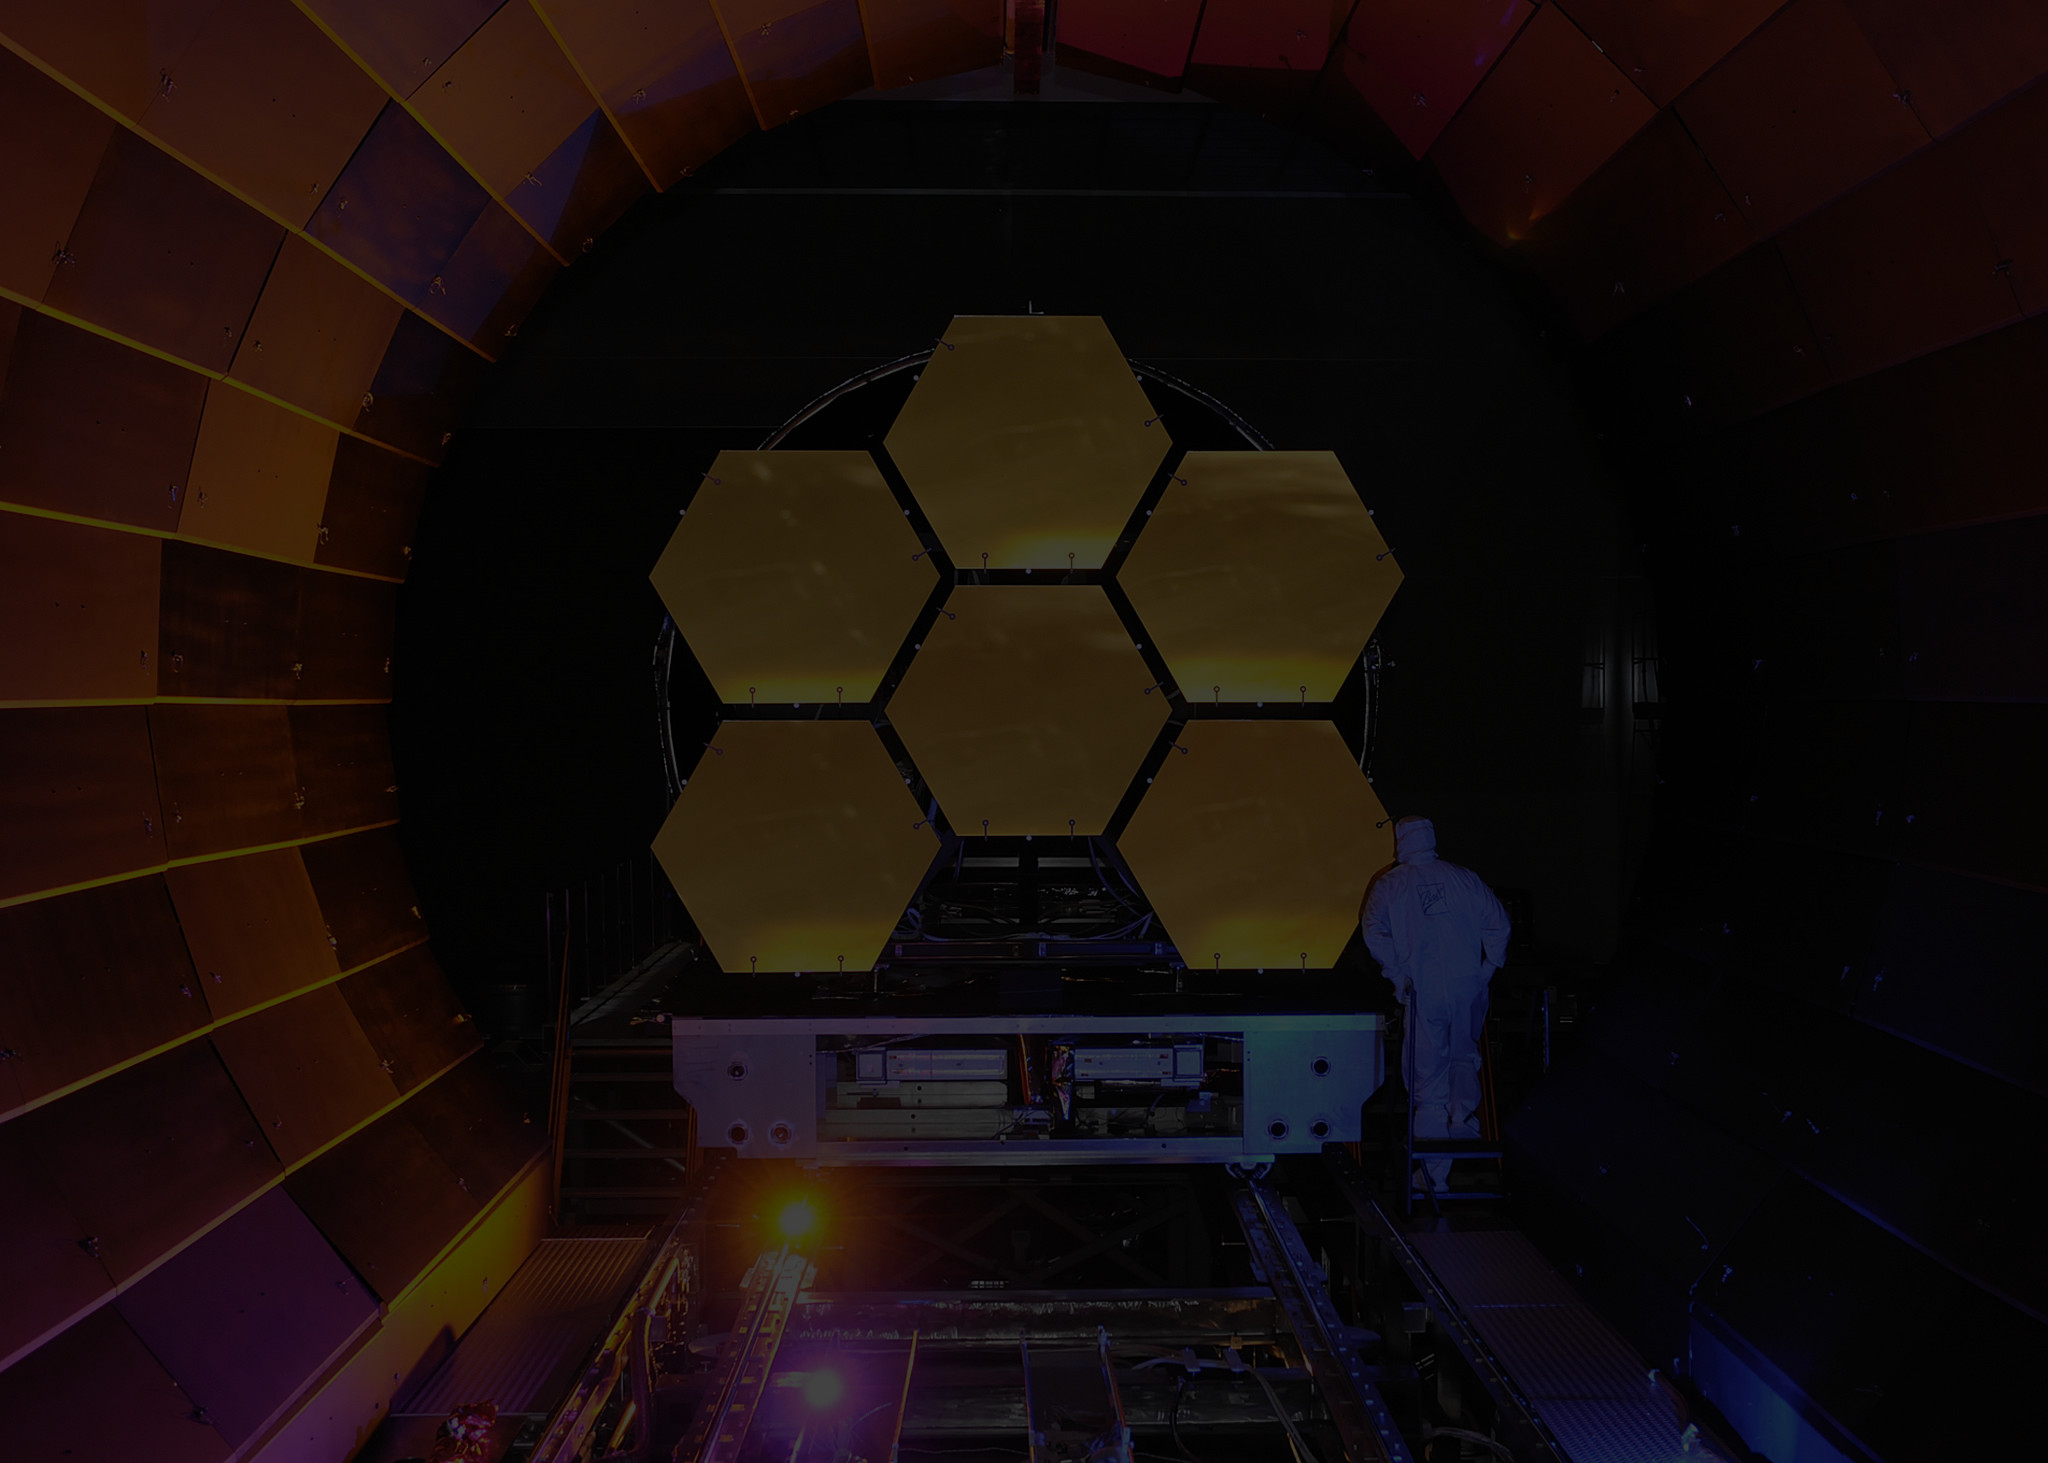
\includegraphics[width=1.2\paperwidth]{figures/jwst_mirror_dark.jpg}\hfil}\vfil}
  % 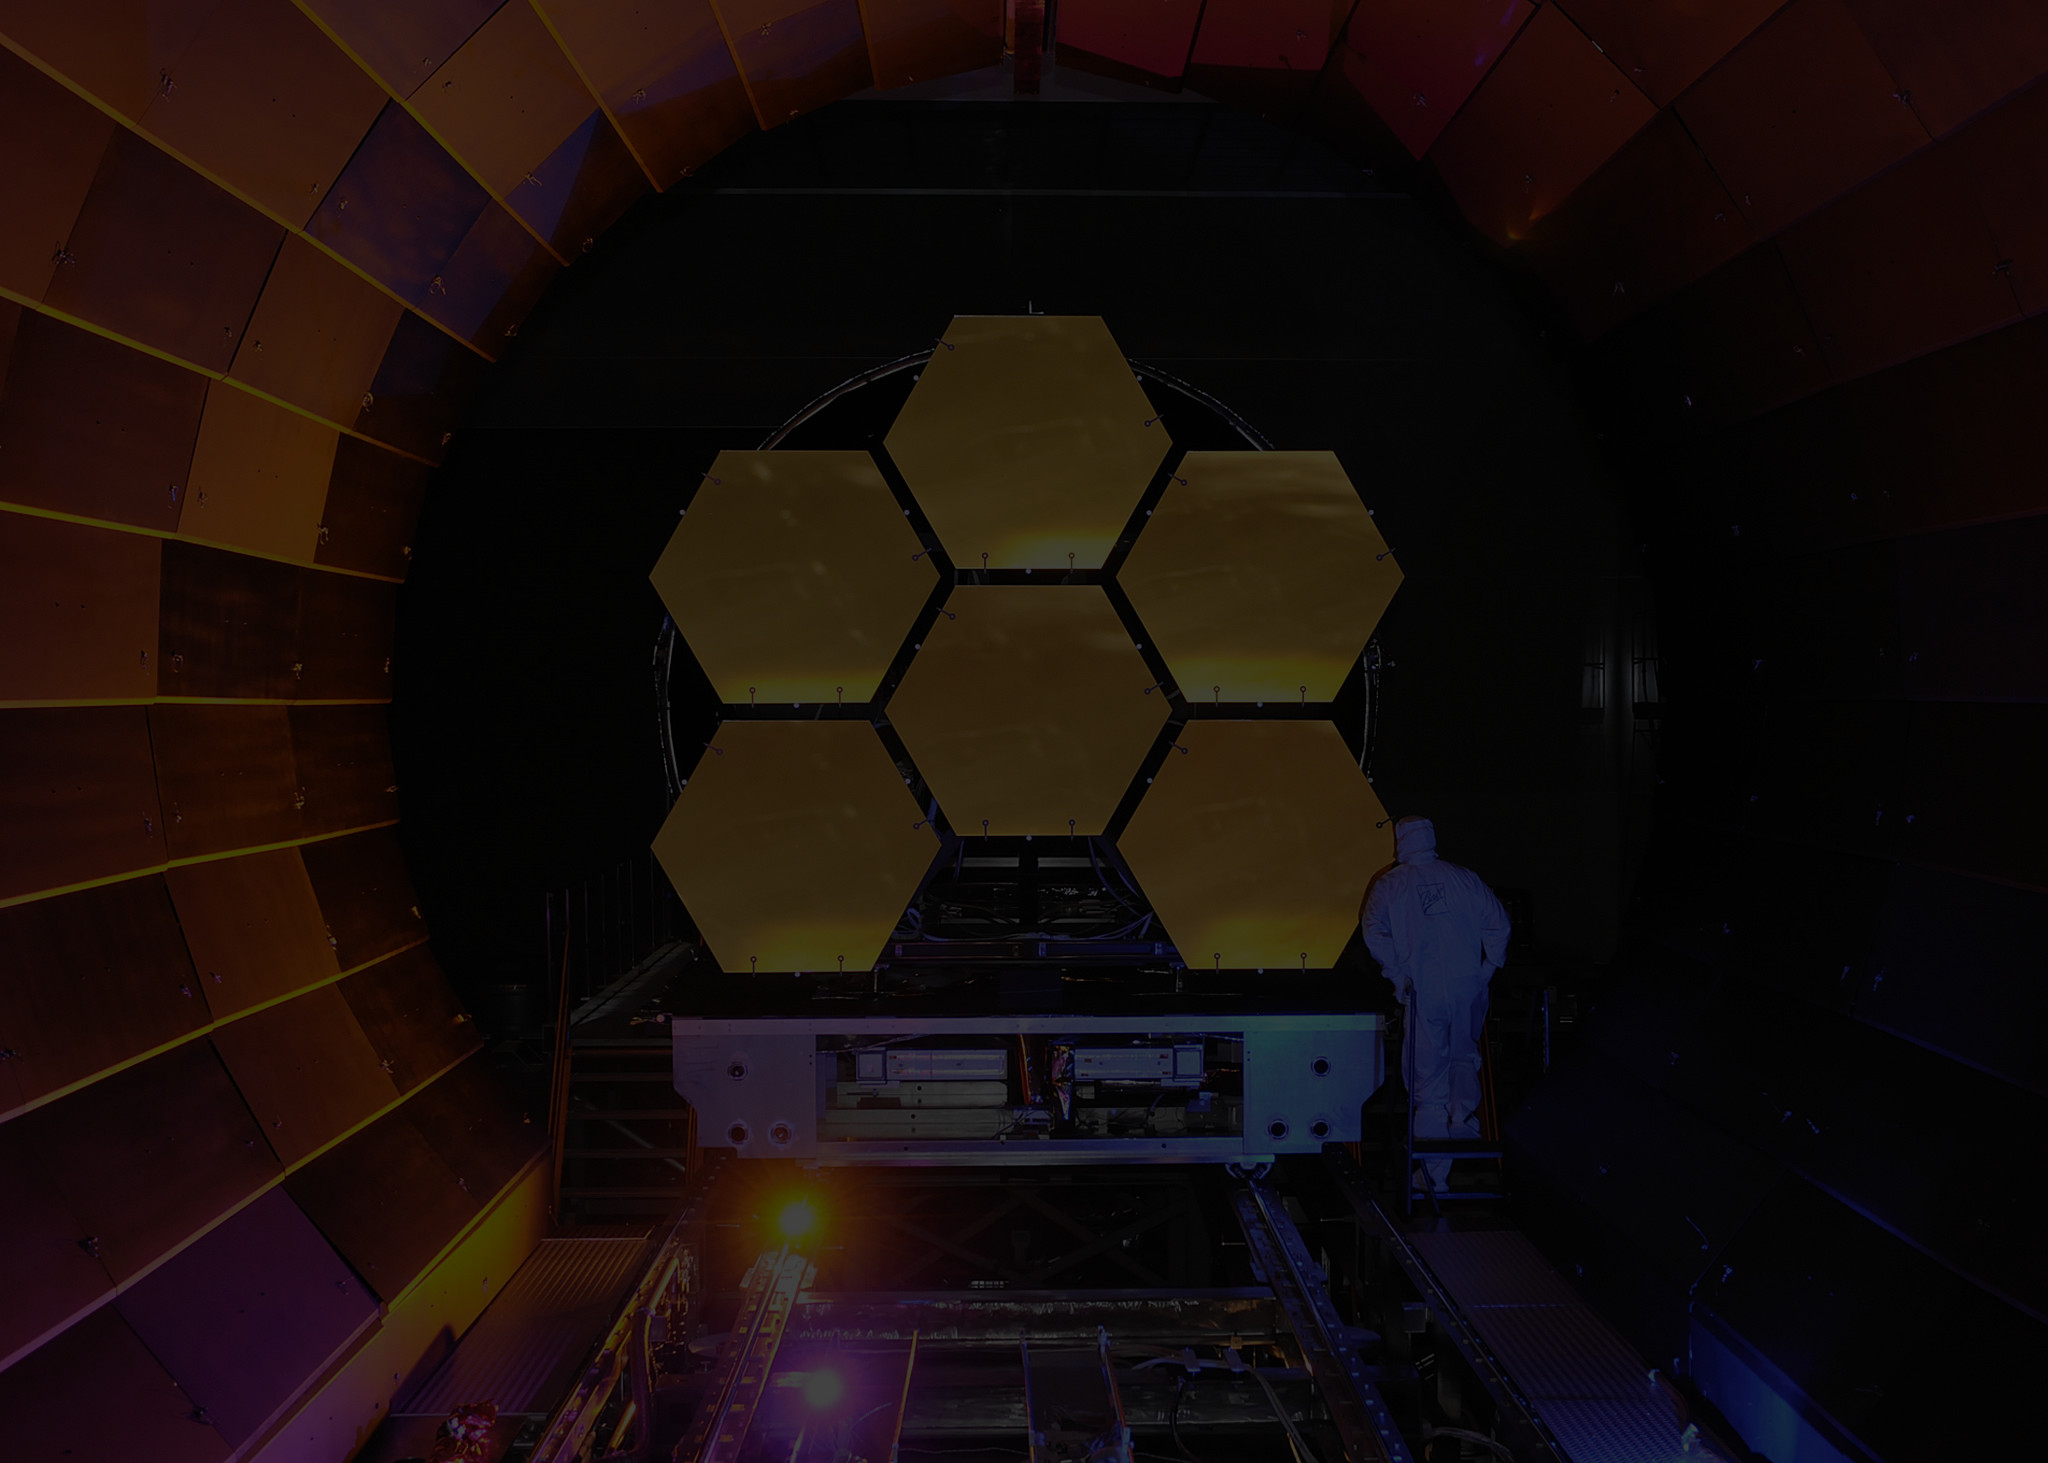
\includegraphics[width=1.2\paperwidth]{figures/jwst_mirror_dark.jpg}
}
\maketitle
}

% \begin{frame}{}
%   \setbeamertemplate{section in toc}[sections numbered]
%   \tableofcontents
% \end{frame}

% \section{Motivation}

%% Imaging planets is hard
\begin{frame}
  \centering
  \Huge
  Imaging planets is hard
\end{frame}

%% Fundamentally, if we beat other errors such as atm, still limited by size of our
%% telescope
\begin{frame}
  \Huge
  Diffraction limit:
  \centering
  \begin{equation*}
    \theta \sim \lambda / D
  \end{equation*}
\end{frame}

%% If ovserve point source, do not get just the point,
%% have PSF : spreading over space so would block point source right next to it
\begin{frame}{}
  \begin{center}
    \LARGE
    Even with JWST ...
    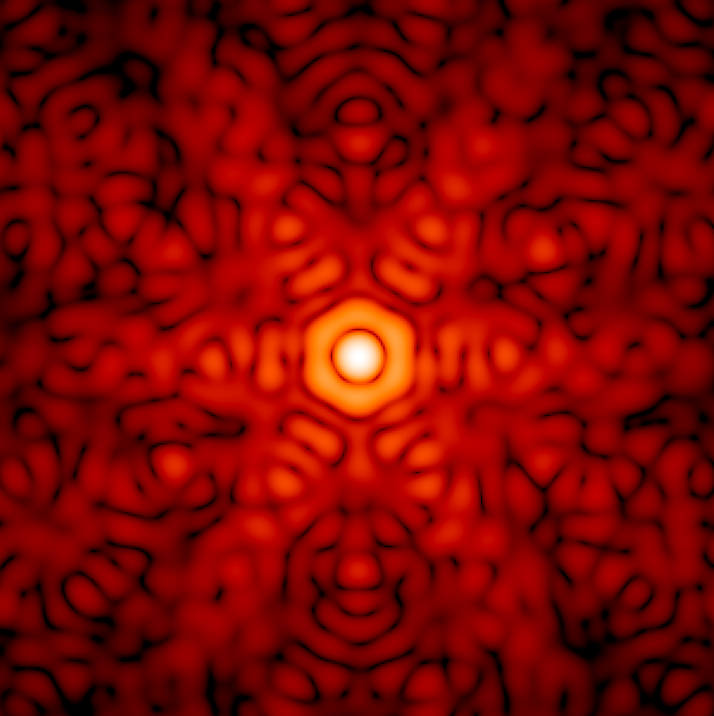
\includegraphics[width=0.7\linewidth]{figures/clearp_psf.png}
  \end{center}
\end{frame}

\begin{frame}{What can we do?}
  \large
  \begin{wideitemize}
    \item Coronagraphy (Inner working angle $\sim$ 0.4-0.6")
    \item \textbf{NIRISS Aperture Masking Interfomertry (AMI)}
  \end{wideitemize}
\end{frame}

%% Aperture: what bullets say
%% Counter intuitive that by blocking most of the light, you get better resolution
\begin{frame}{Non-redundant mask}

  \begin{center}
    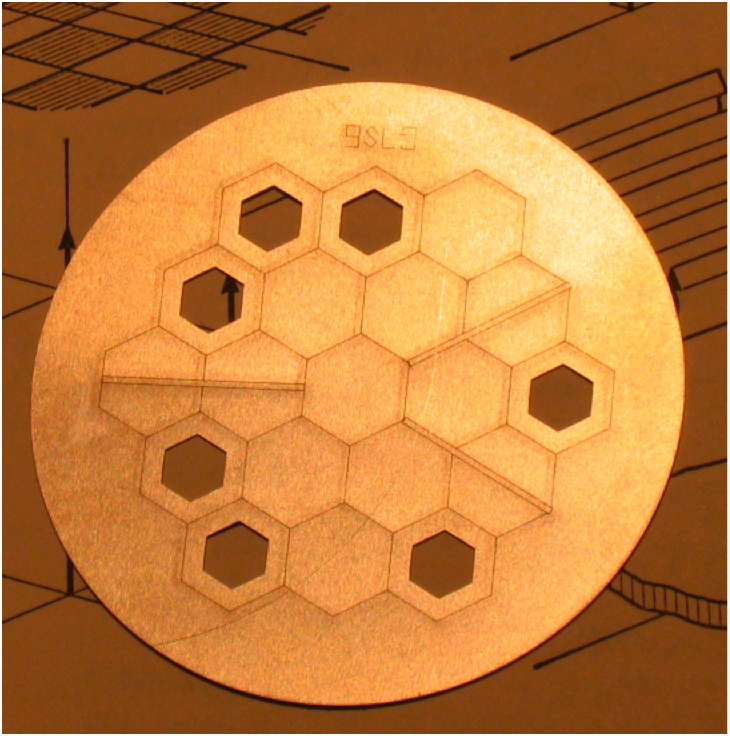
\includegraphics[width=0.6\linewidth]{figures/AMI_mask_prototype.jpg}
  \end{center}

  \footnotesize Image: Anand Sivaramakrishnan
\end{frame}

\begin{frame}{NIRISS Clear Pupil}

  \begin{center}
    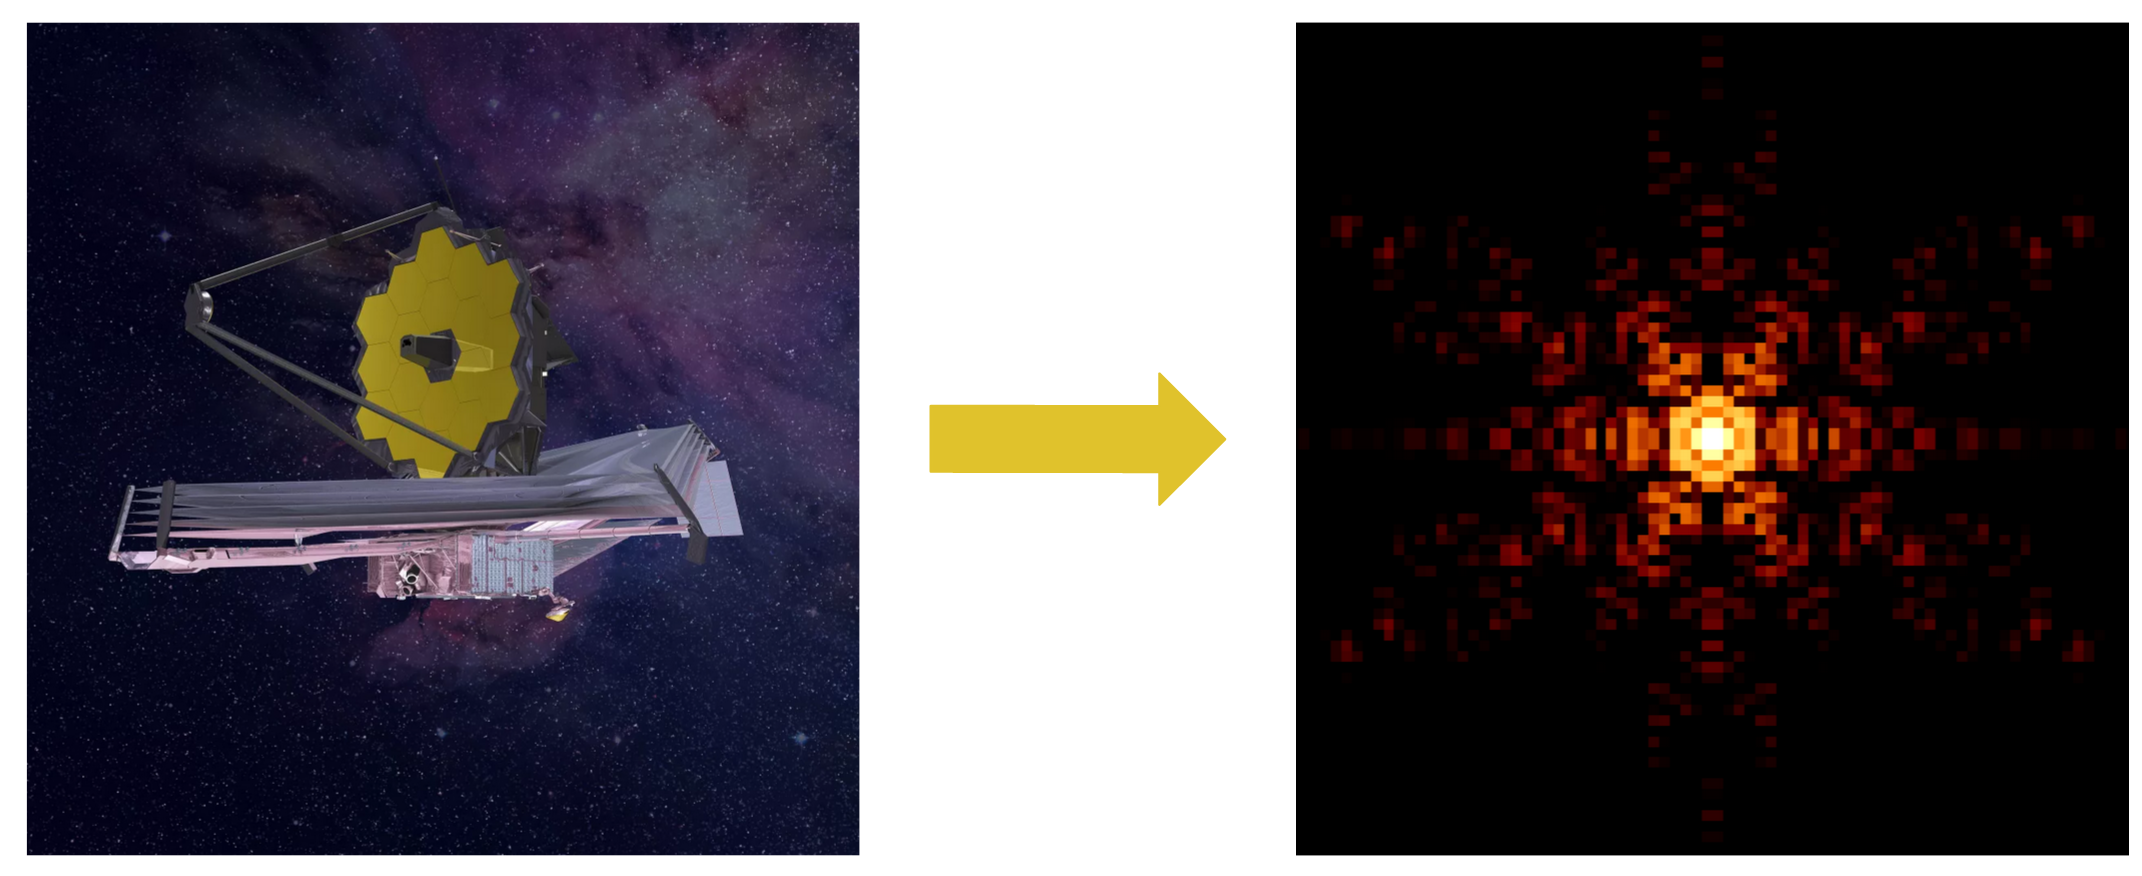
\includegraphics[width=\linewidth]{figures/webb_and_psf.png}
  \end{center}

  \footnotesize Image: NASA
\end{frame}

\begin{frame}{NIRISS AMI}

  \begin{center}
    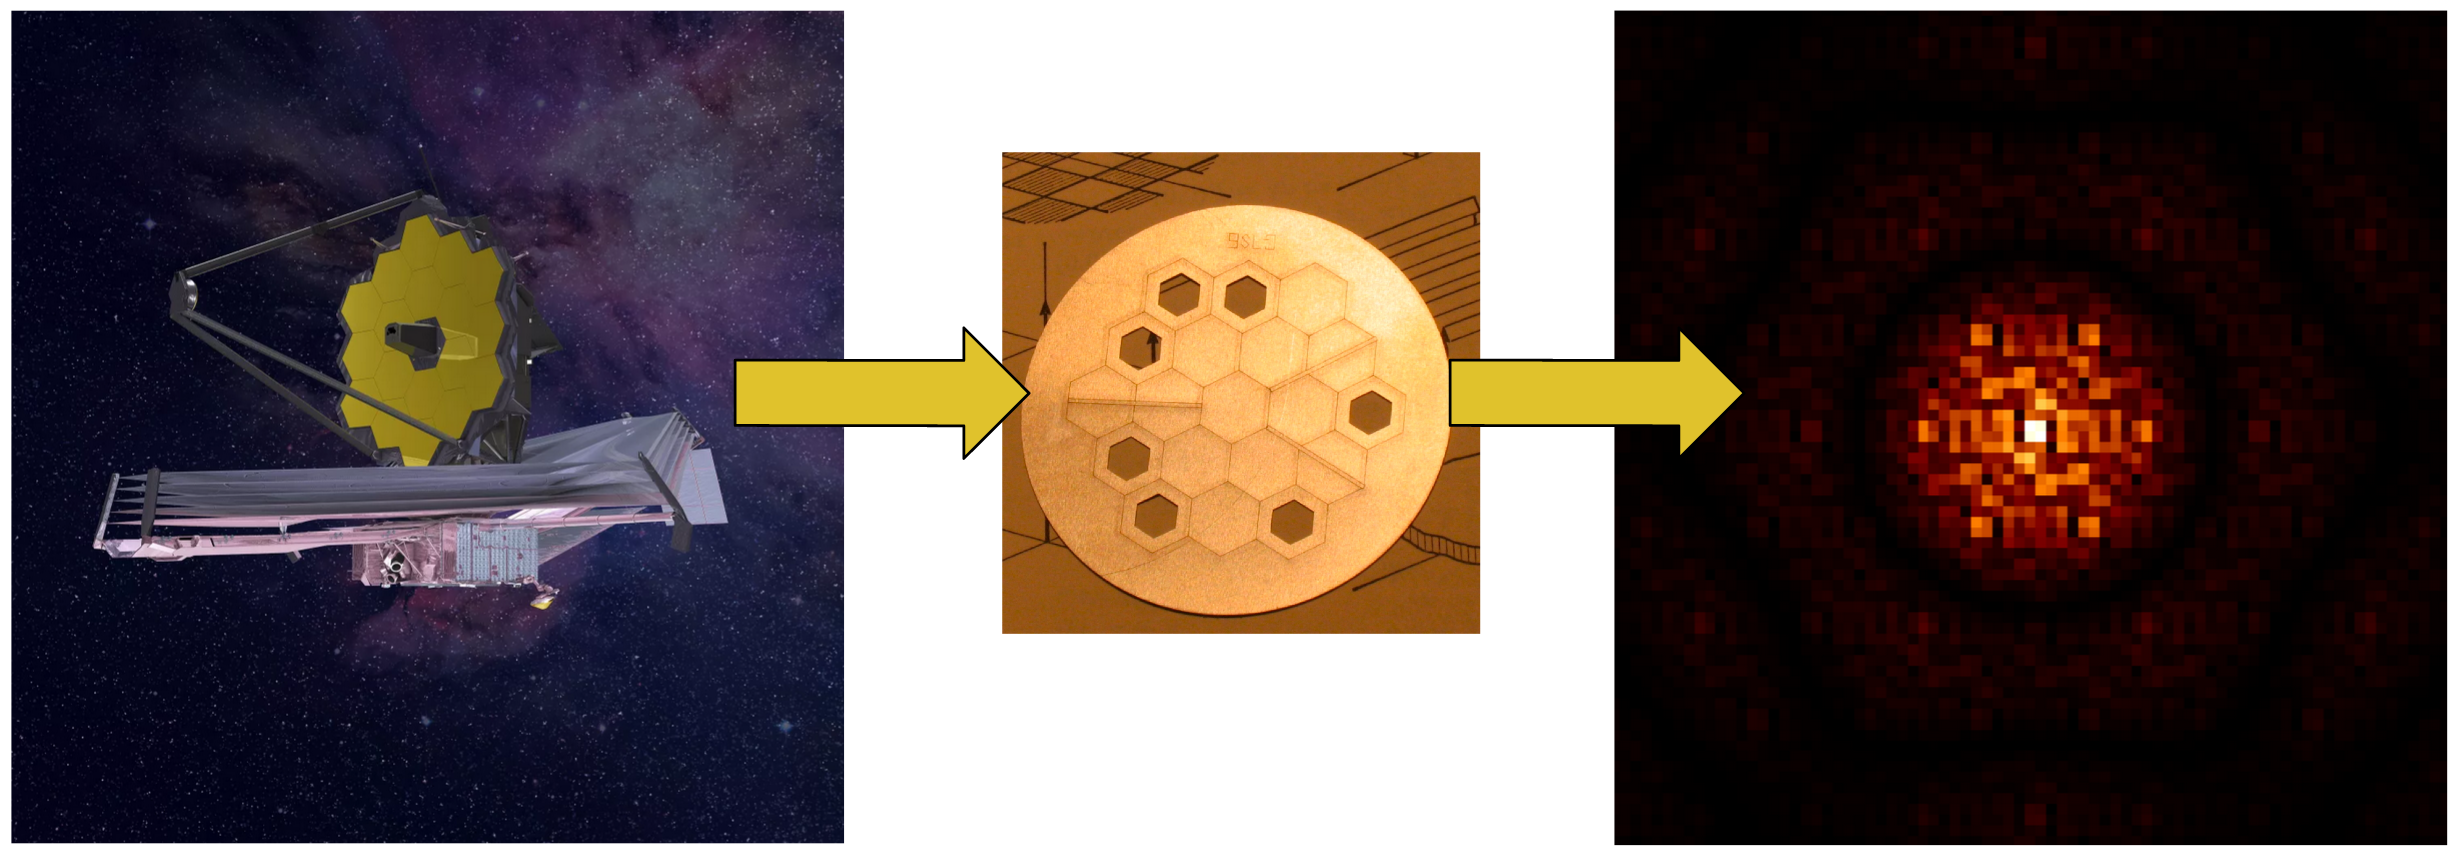
\includegraphics[width=\linewidth]{figures/webb_and_ami.png}
  \end{center}

  \footnotesize Images: NASA, Anand Sivaramakrishnan
\end{frame}

\begin{frame}{Clear Pupil vs AMI Mask}
  \begin{center}
    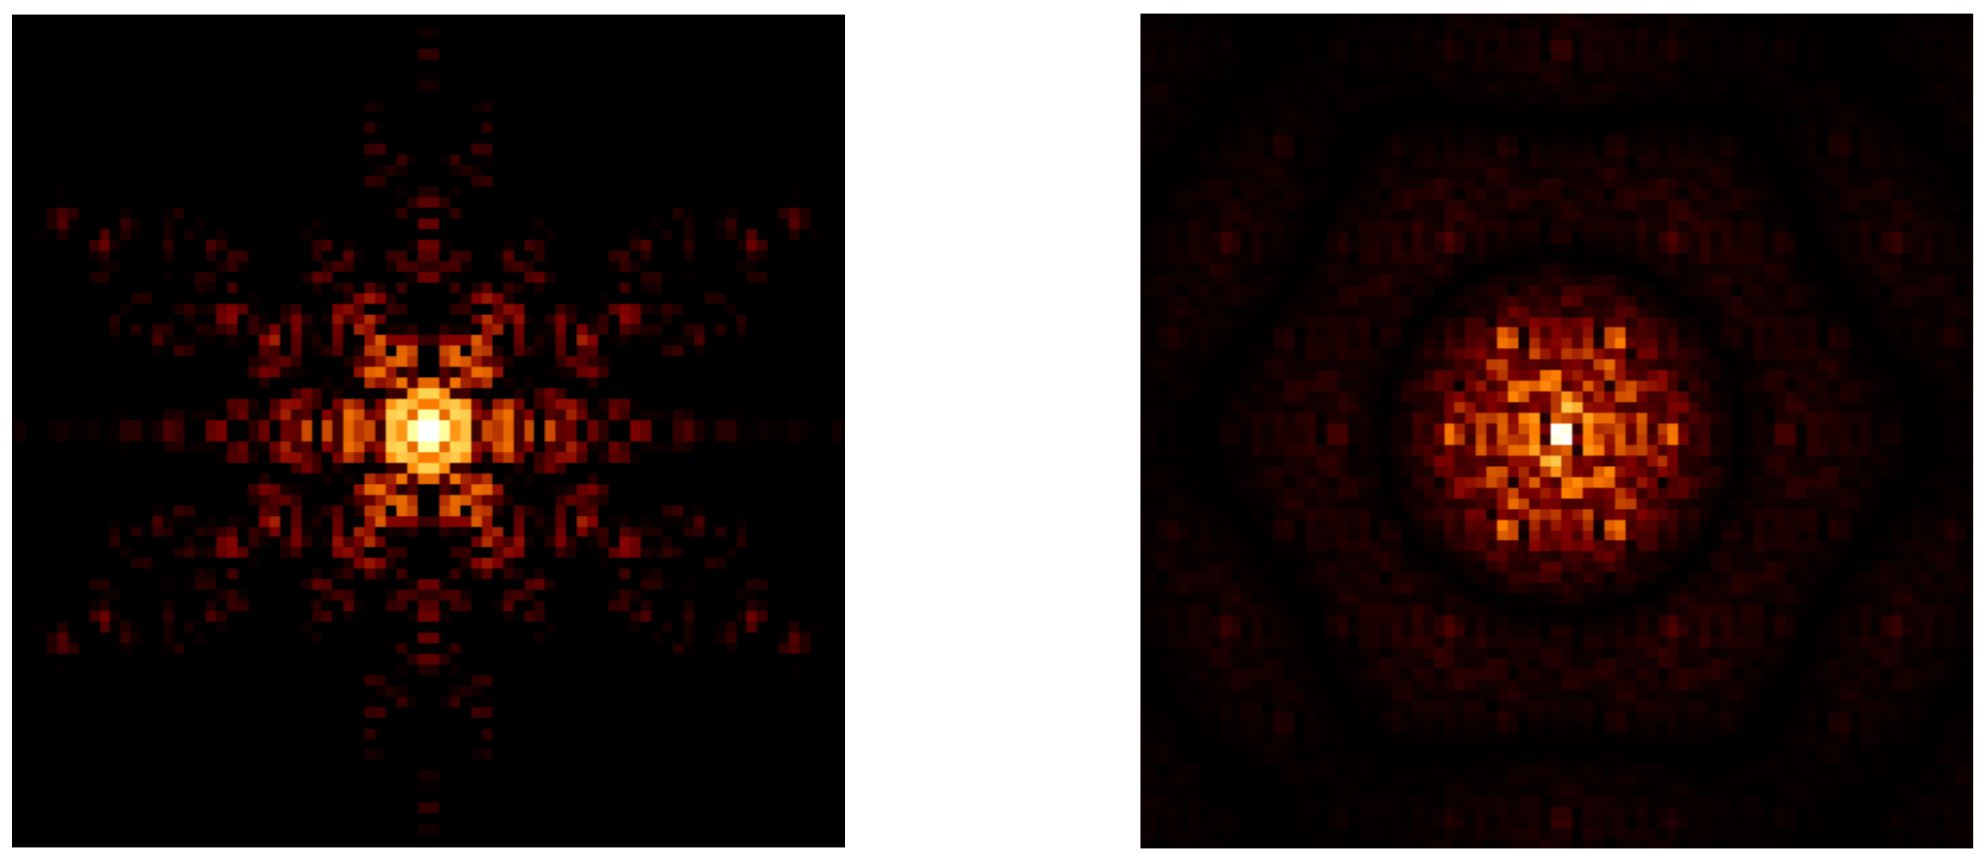
\includegraphics[width=\linewidth]{figures/clear_vs_ami.png}
  \end{center}
\end{frame}

%% In real life, not just pupil -> PSF
% Imagine have star near core
% Now, narrower core, focusing on high spatial frequencies
% \begin{frame}{Wavefront errors}
%   \begin{center}
%     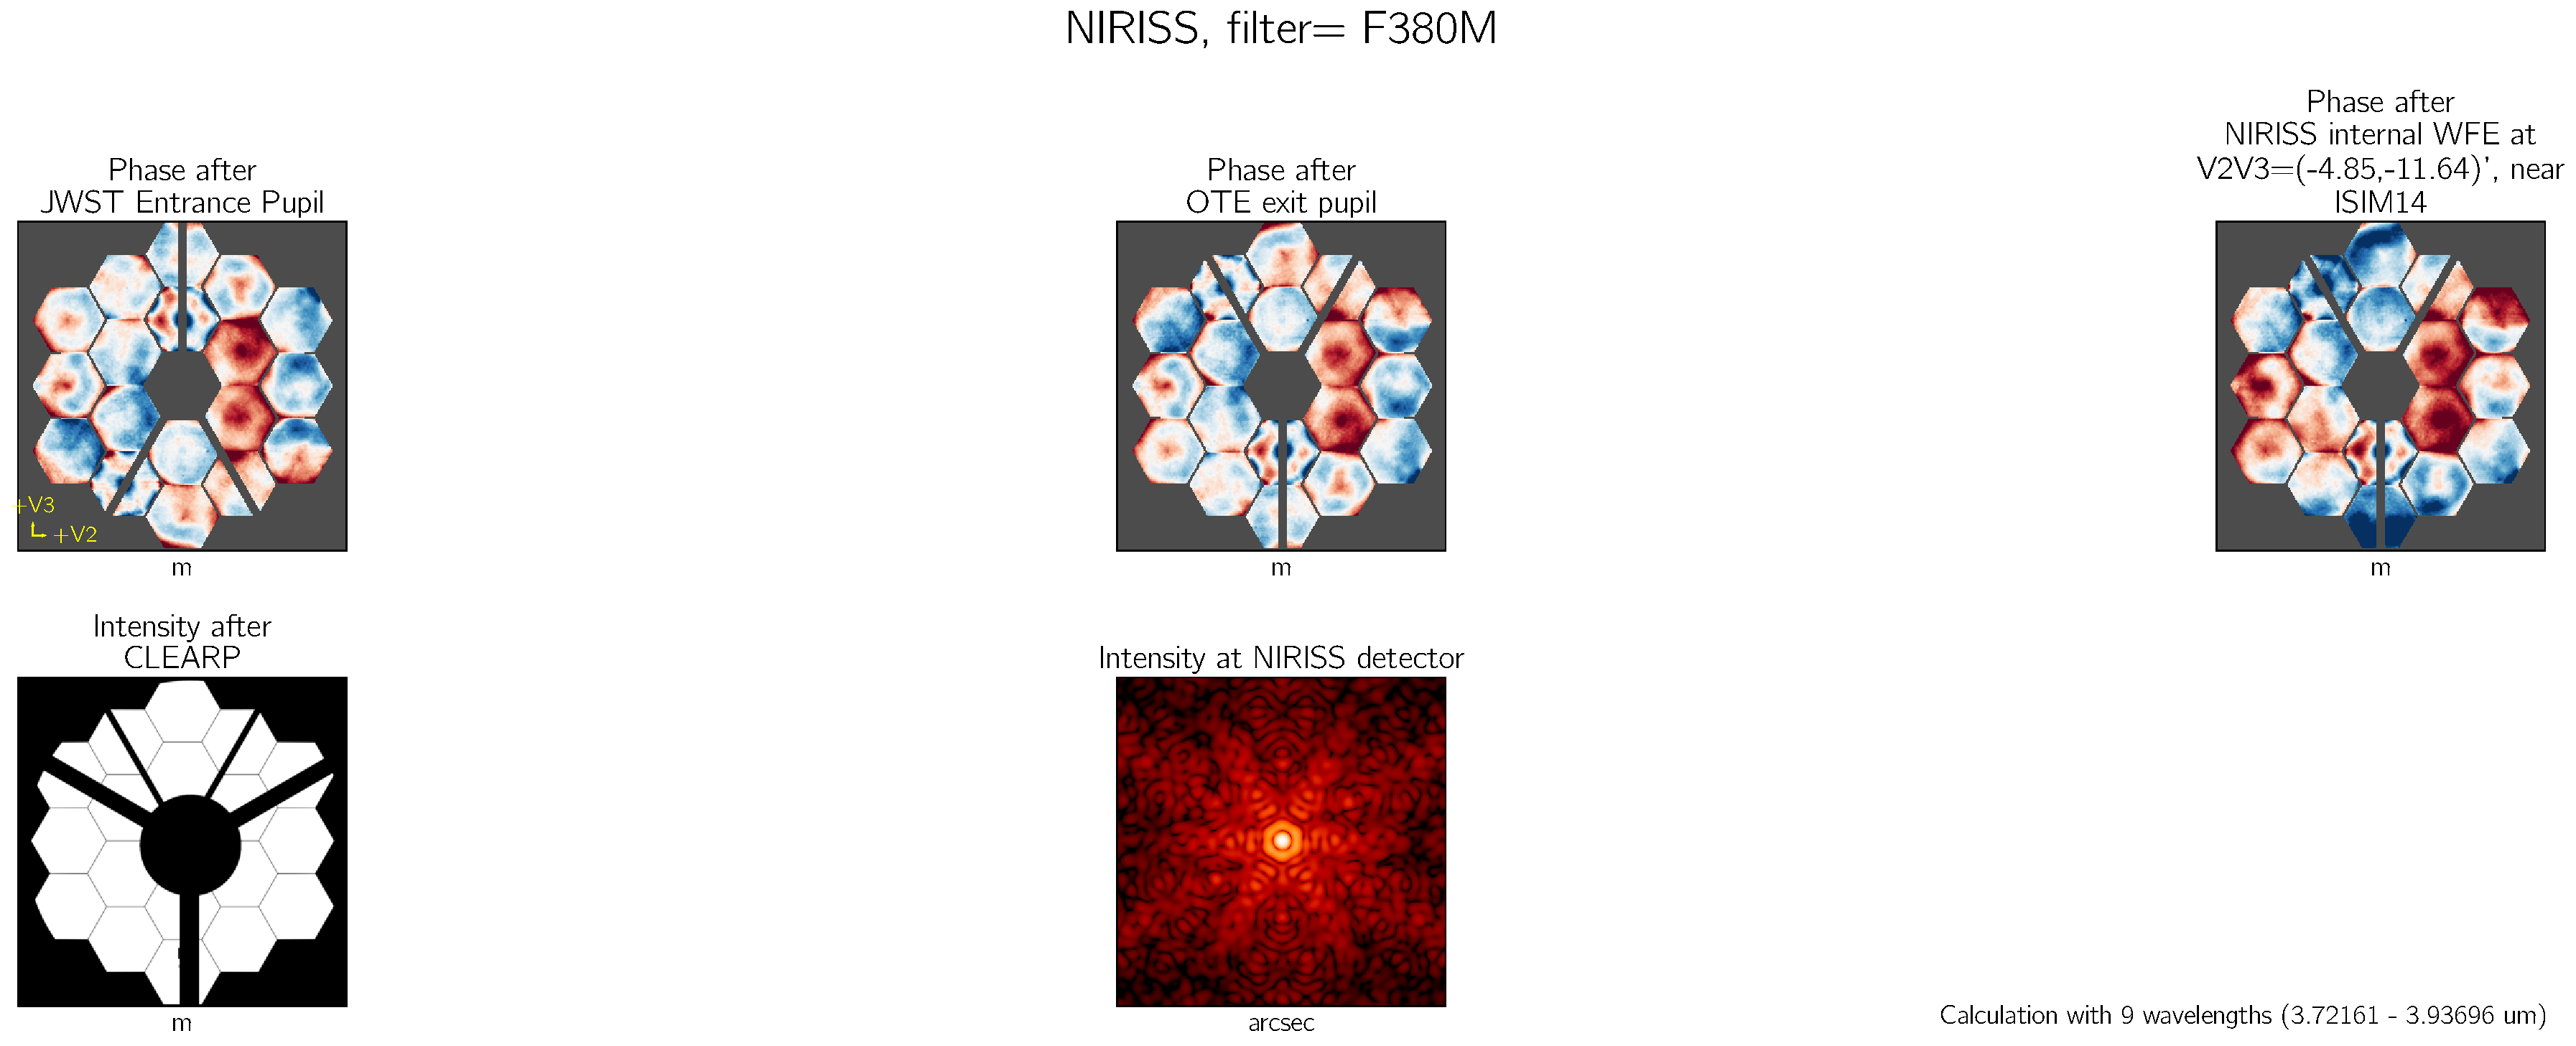
\includegraphics[width=\linewidth]{figures/webbpsf_clear.pdf}
%   \end{center}
% \end{frame}

%% The generic idea is that instead of letting it blend in full pupil, we single
%% out errors in each hole -> Then can correct
% TODO: Nicer WebbPSF images
% \begin{frame}{Wavefront errors}
%   %% NOTE: Don't combine random error phases -> Cool !
%   Each pair of apertures probes a unique baseline: \textit{non-redundant} masking
%   \begin{center}
%     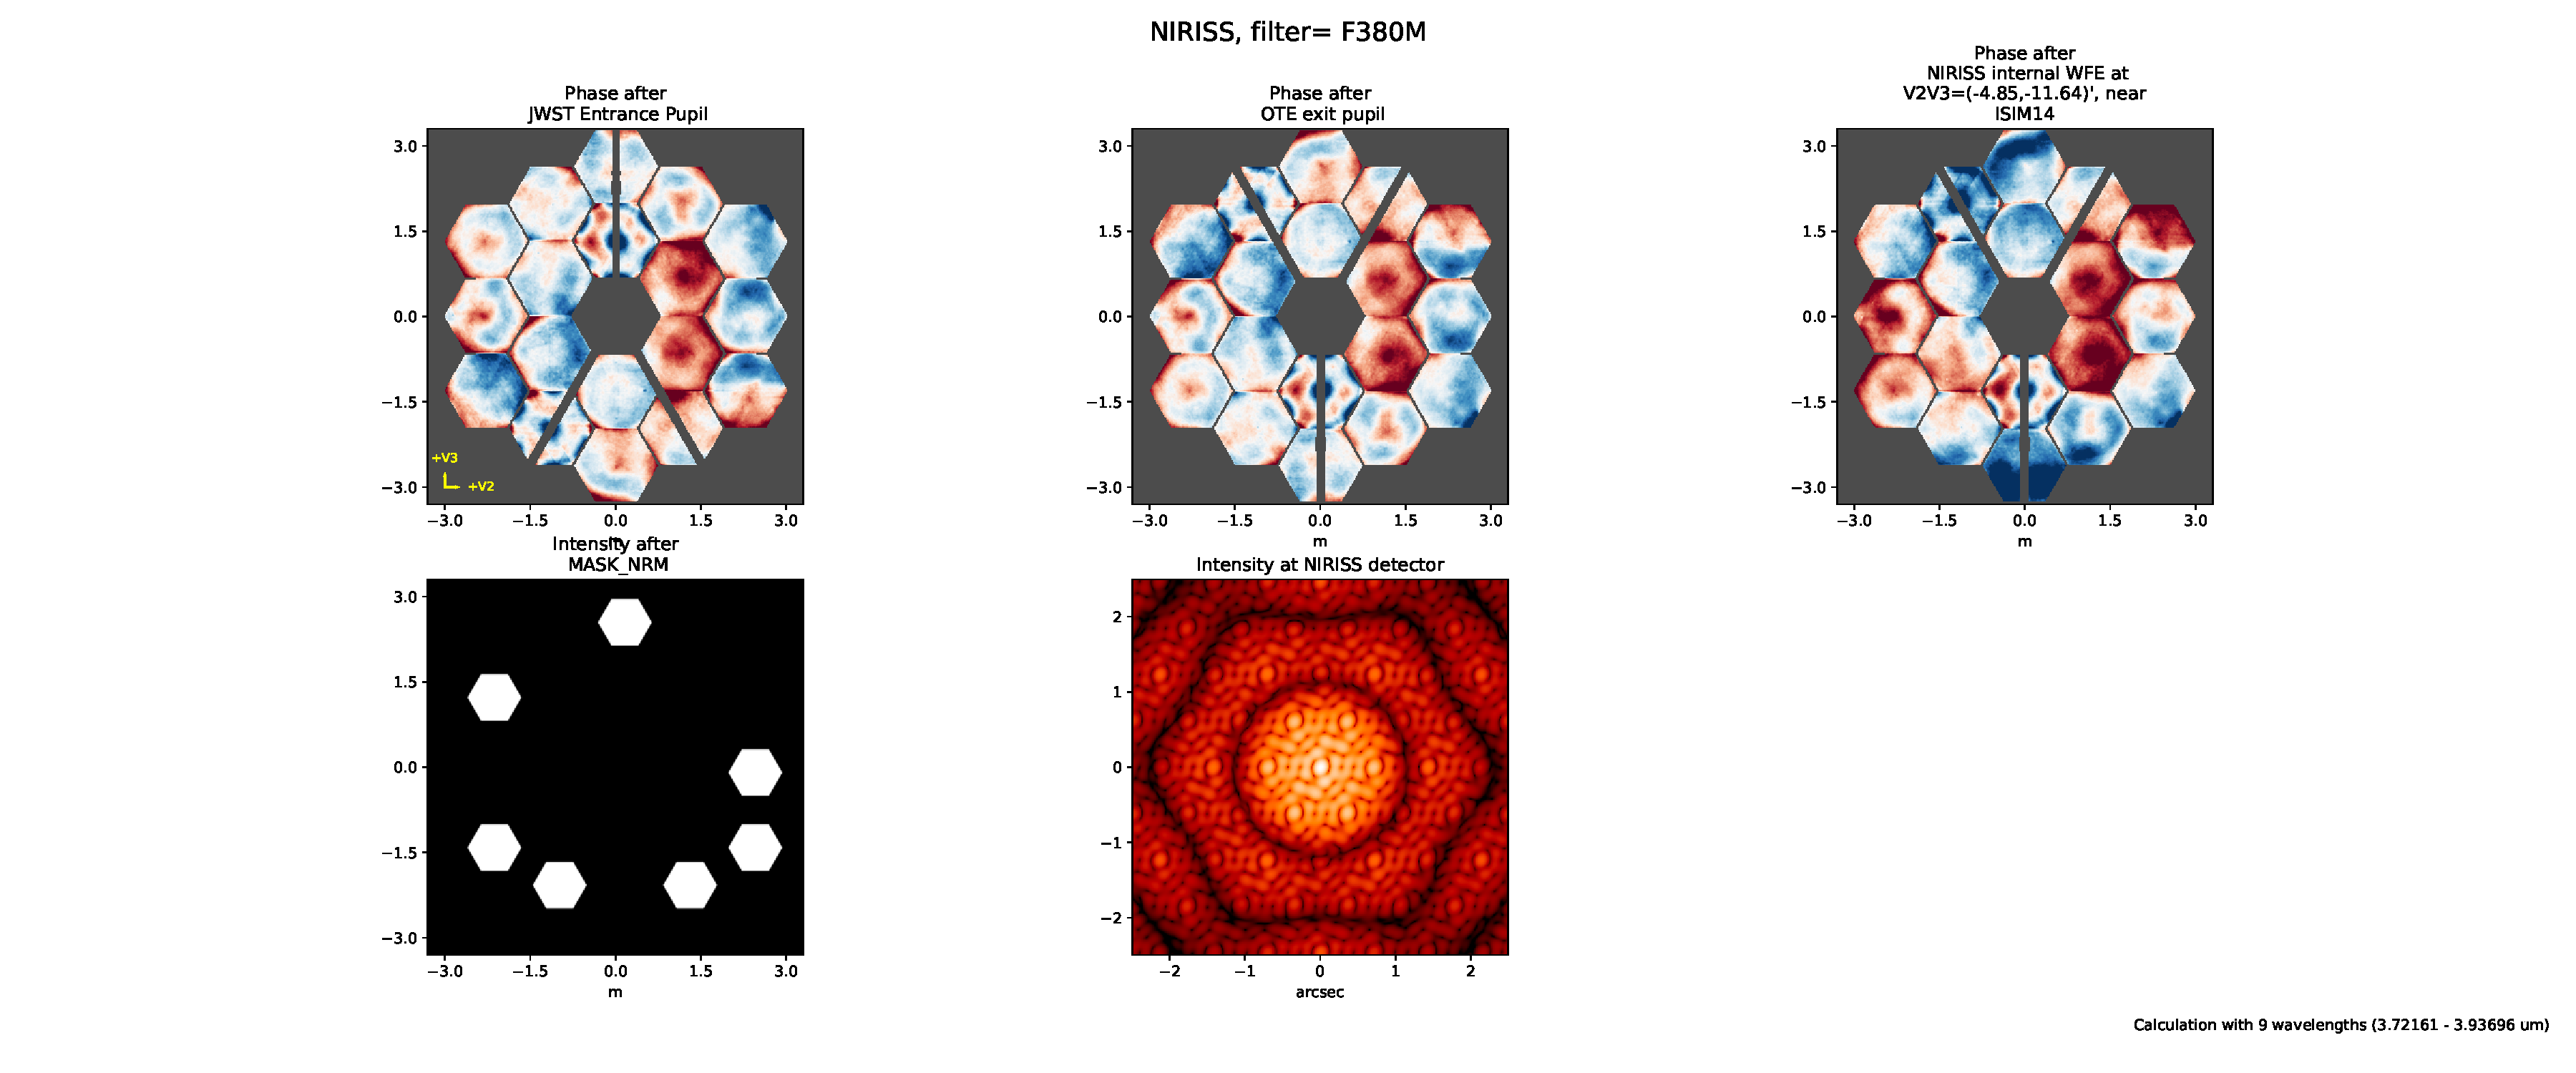
\includegraphics[width=\linewidth]{figures/webbpsf_ami.pdf}
%   \end{center}
% \end{frame}

% \begin{frame}{From the FT of the PSF, we have phases}
%   \begin{center}
%     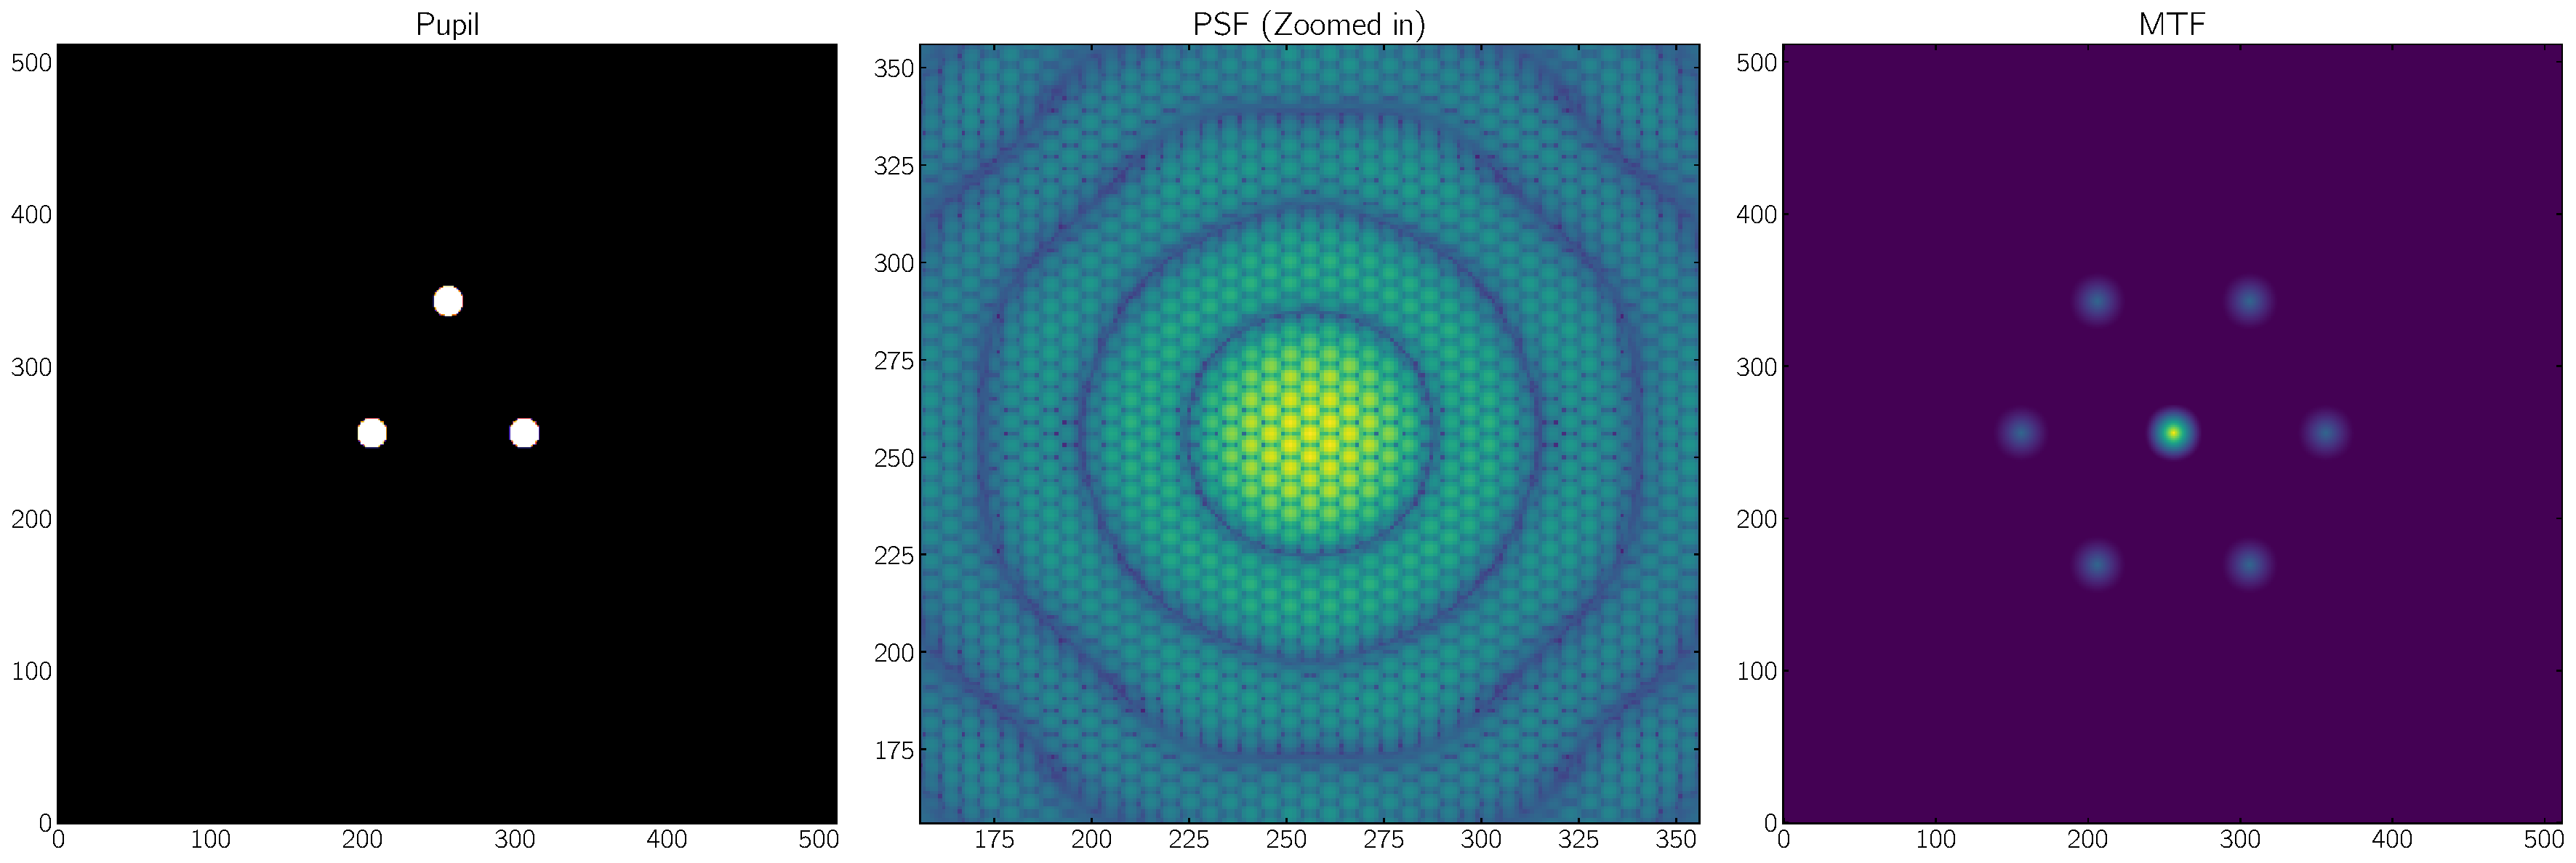
\includegraphics[width=\linewidth]{figures/analyse_three_apertures.pdf}
%   \end{center}
%
%   Each peak in the MTF comes from two apertures (1 and 2). Its phase is
%   \begin{equation*}
%     \Phi_{1,2} = \Phi_{1,2}^O + \phi_2 - \phi_1
%   \end{equation*}
% \end{frame}

% \begin{frame}{Phases for a triangle}
%
% \begin{columns}
% \column{0.6\textwidth}
%
%   \begin{align*}
%     &\Phi_{1,2} = \Phi_{1,2}^O + \phi_2 - \phi_1 \\
%     &\Phi_{2,3} = \Phi_{2,3}^O + \phi_3 - \phi_2 \\
%     &\Phi_{3,1} = \Phi_{3,1}^O + \phi_1 - \phi_3
%   \end{align*}
%
% \column{0.4\textwidth}
%   \onslide<1->{
%     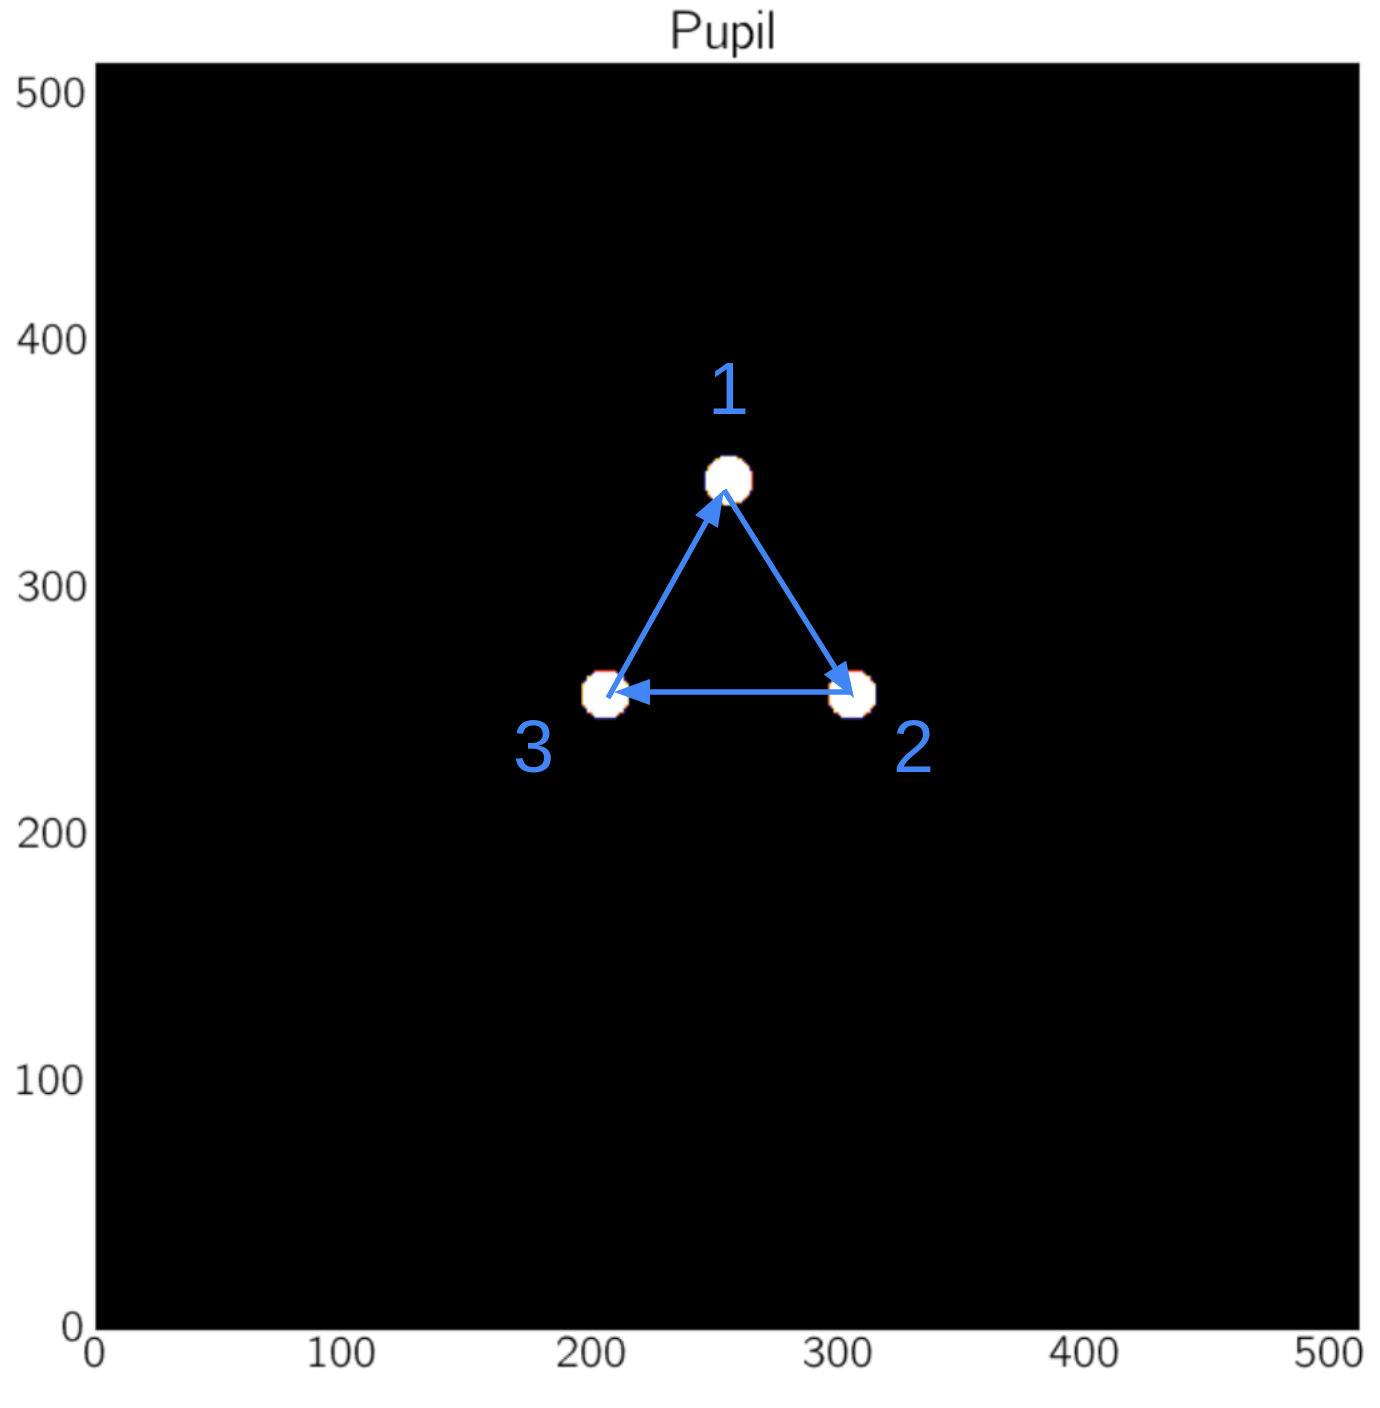
\includegraphics[width=\linewidth]{figures/triangle_arrows.png}
%   }
% \end{columns}
%
% \end{frame}


% \begin{frame}{Phases for a triangle}
%
% Take $\phi_1 = 0$ as a reference
%
% \begin{columns}
% \column{0.6\textwidth}
%
%   \only<1>{
%     \begin{align*}
%       &\Phi_{1,2} = \Phi_{1,2}^O + \phi_2 \\
%       &\Phi_{2,3} = \Phi_{2,3}^O + \phi_3 - \phi_2 \\
%       &\Phi_{3,1} = \Phi_{3,1}^O - \phi_3
%     \end{align*}
%   }
%   \only<2->{
%     \begin{align*}
%       &\Phi_{1,2} = \Phi_{1,2}^O + \cancel{\phi_2} \\
%       &\Phi_{2,3} = \Phi_{2,3}^O + \cancel{\phi_3} - \cancel{\phi_2} \\
%       &\Phi_{3,1} = \Phi_{3,1}^O - \cancel{\phi_3}
%     \end{align*}
%   }
%
%
%   \onslide<3->{
%     \begin{equation*}
%       C_{123} = \Phi_{1,2} + \Phi_{2,3} + \Phi_{3,1} = \Phi_{1,2}^O + \Phi_{2,3}^O + \Phi_{3,1}^O
%     \end{equation*}
%   }
%
%
% \column{0.4\textwidth}
%   \onslide<1->{
%     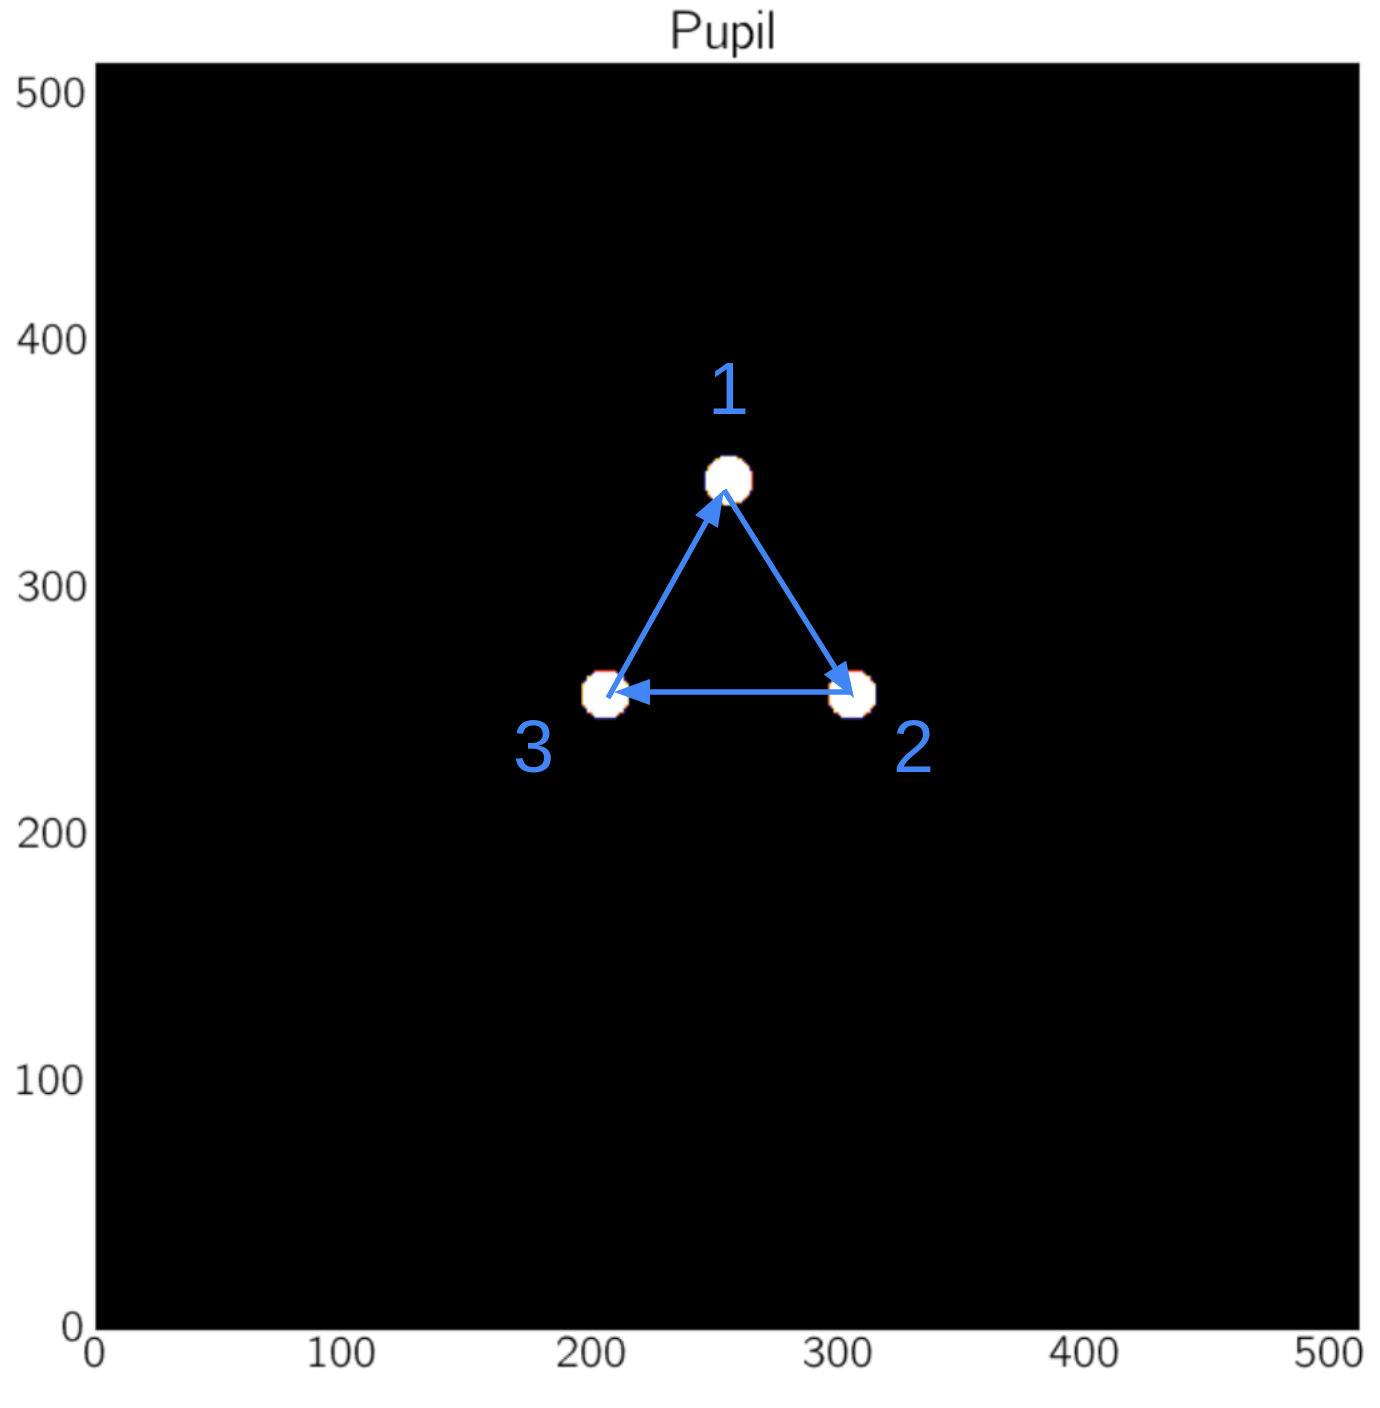
\includegraphics[width=\linewidth]{figures/triangle_arrows.png}
%   }
% \end{columns}
%
% \end{frame}
%
%
% \begin{frame}{Closure phase}
%
% \begin{columns}
% \column{0.6\textwidth}
%
%   \only<1>{
%     \begin{align*}
%       &\Phi_{1,2} = \Phi_{1,2}^O + \phi_2 \\
%       &\Phi_{2,3} = \Phi_{2,3}^O + \phi_3 - \phi_2 \\
%       &\Phi_{3,1} = \Phi_{3,1}^O - \phi_3
%     \end{align*}
%   }
%   \only<2->{
%     \begin{align*}
%       &\Phi_{1,2} = \Phi_{1,2}^O + \cancel{\phi_2} \\
%       &\Phi_{2,3} = \Phi_{2,3}^O + \cancel{\phi_3} - \cancel{\phi_2} \\
%       &\Phi_{3,1} = \Phi_{3,1}^O - \cancel{\phi_3}
%     \end{align*}
%   }
%
%
%   \begin{equation*}
%     C_{123} = \Phi_{1,2} + \Phi_{2,3} + \Phi_{3,1} = \Phi_{1,2}^O + \Phi_{2,3}^O + \Phi_{3,1}^O
%   \end{equation*}
%
% \column{0.4\textwidth}
%   \onslide<1->{
%     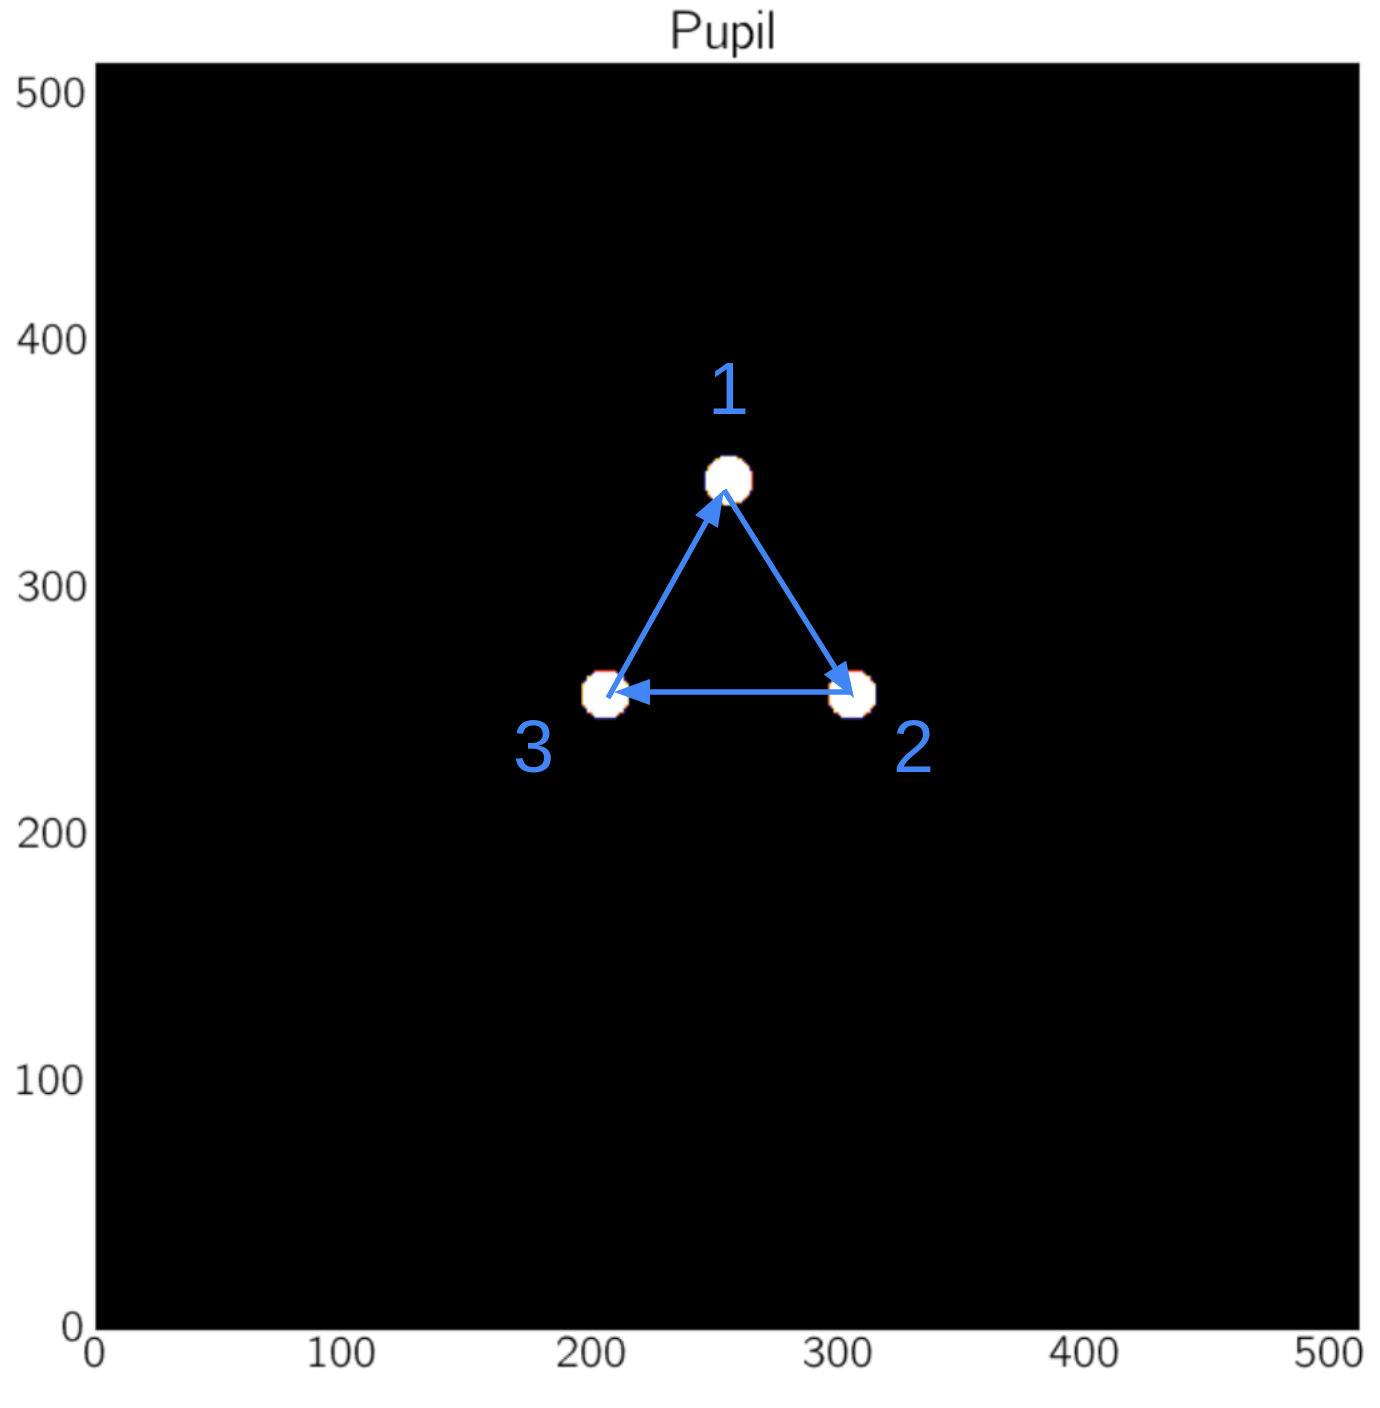
\includegraphics[width=\linewidth]{figures/triangle_arrows.png}
%   }
% \end{columns}
%
% \end{frame}


% \begin{frame}{Example binary}
%   \begin{wideitemize}
%     \item<1-> Observe target
%     \item<4-|only@4-> Calculate CP $C_{123} = \Phi_{1,2} + \Phi_{2,3} + \Phi_{3,1} = \Phi_{1,2}^O + \Phi_{2,3}^O + \Phi_{3,1}^O$ for each triangle
%     \item<5-|only@5-> Generate model CP (for example binary or disk) analytically
%     \item<6-|only@6-> Fit model CP to observed CP
%     \item<7-|only@7-> Detect companion below 0.1-0.4" (with JWST/NIRISS)
%   \end{wideitemize}
%   \only<1>{
%     \begin{center}
%       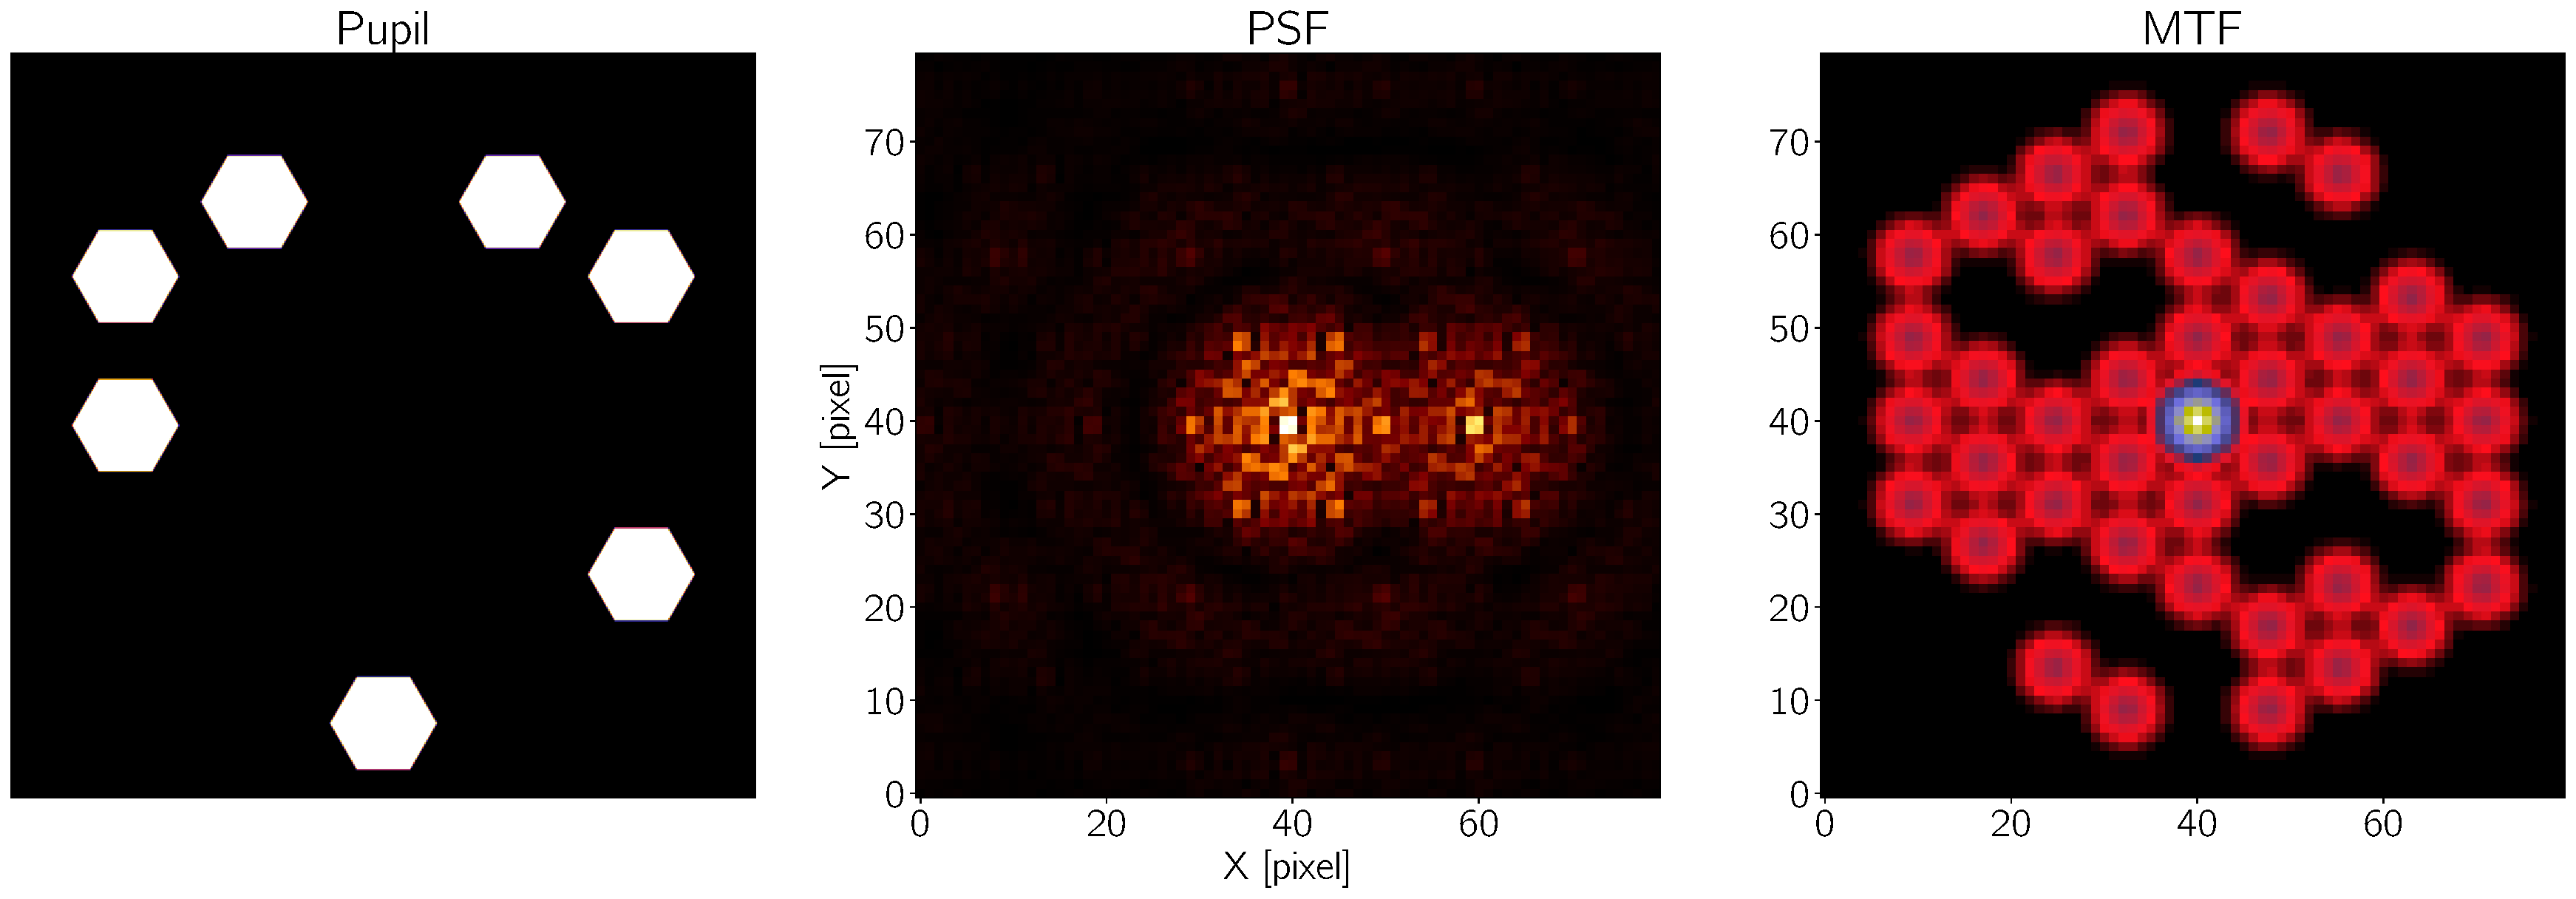
\includegraphics[width=\linewidth]{figures/analyse_niriss_ami_bin_sep_20_cr_0.5.pdf}
%     \end{center}
%   }
%   %% Closer is harder
%   \only<2>{
%     \begin{center}
%       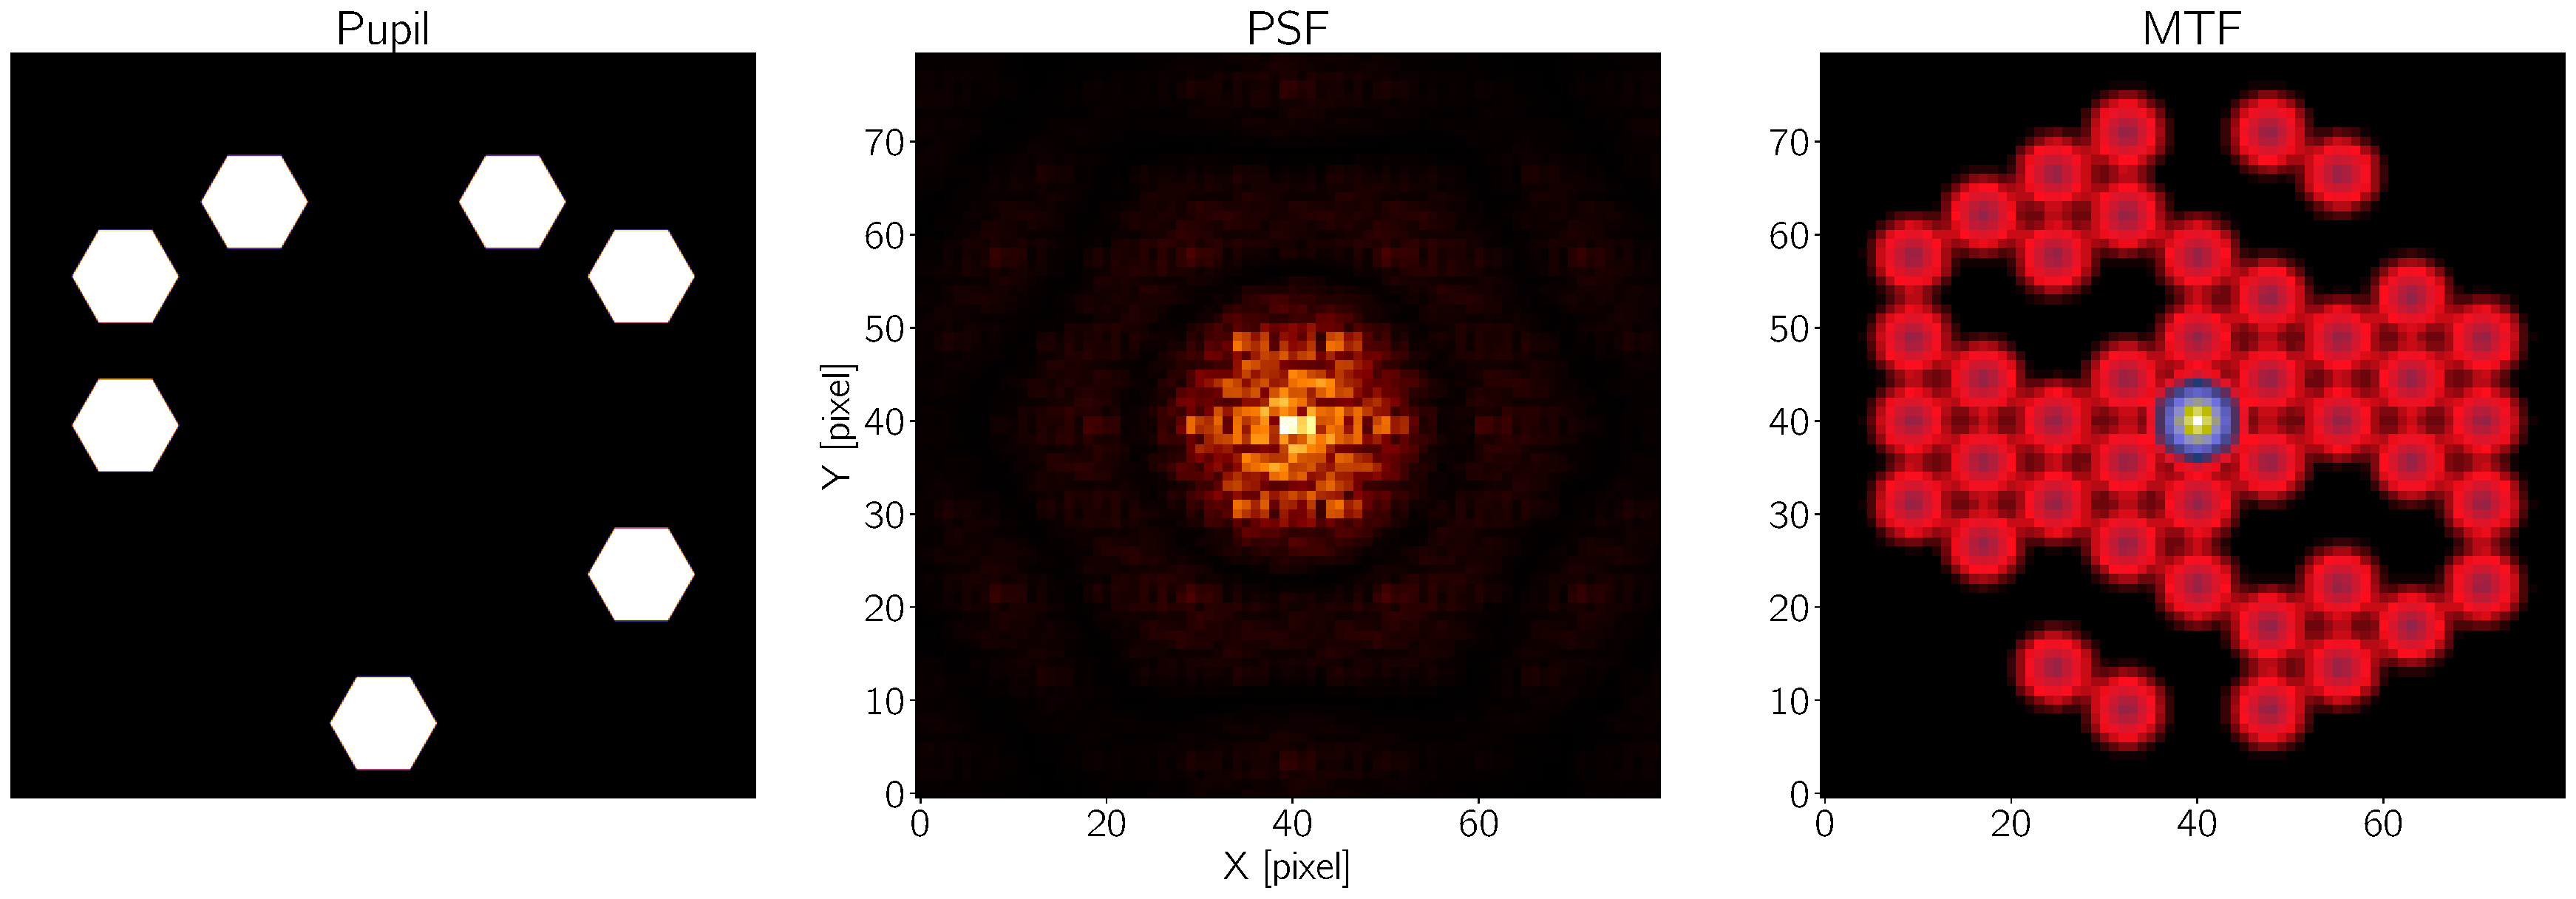
\includegraphics[width=\linewidth]{figures/analyse_niriss_ami_bin_sep_2_cr_0.5.pdf}
%     \end{center}
%   }
%   %% Fainter is harder (now cannot see by eye)
%   \only<3-4>{
%     \begin{center}
%       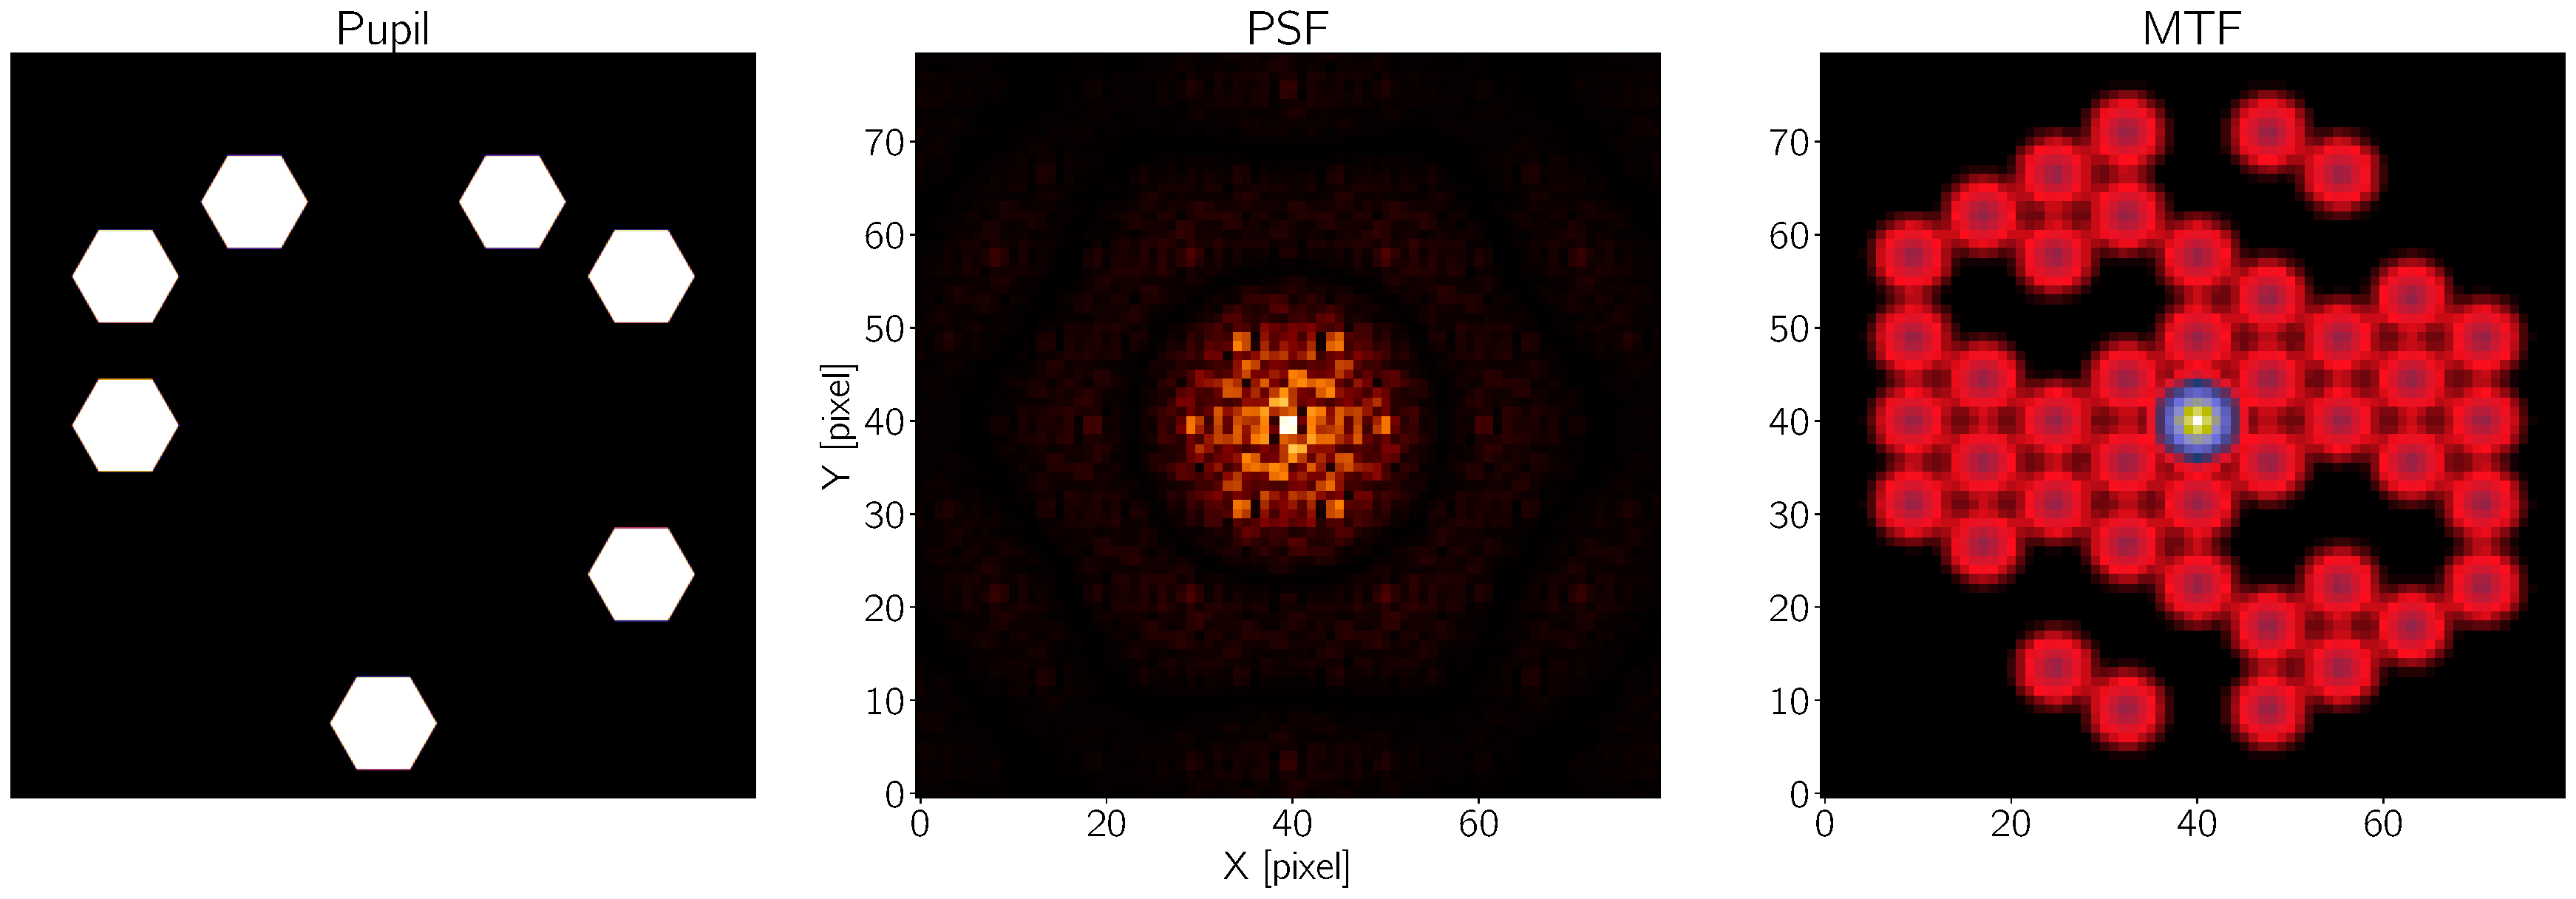
\includegraphics[width=\linewidth]{figures/analyse_niriss_ami_bin_sep_2_cr_0.0001.pdf}
%     \end{center}
%   }
% \end{frame}

\begin{frame}{NIRISS AMI: Single star}
  \only<1>{
    \begin{center}
      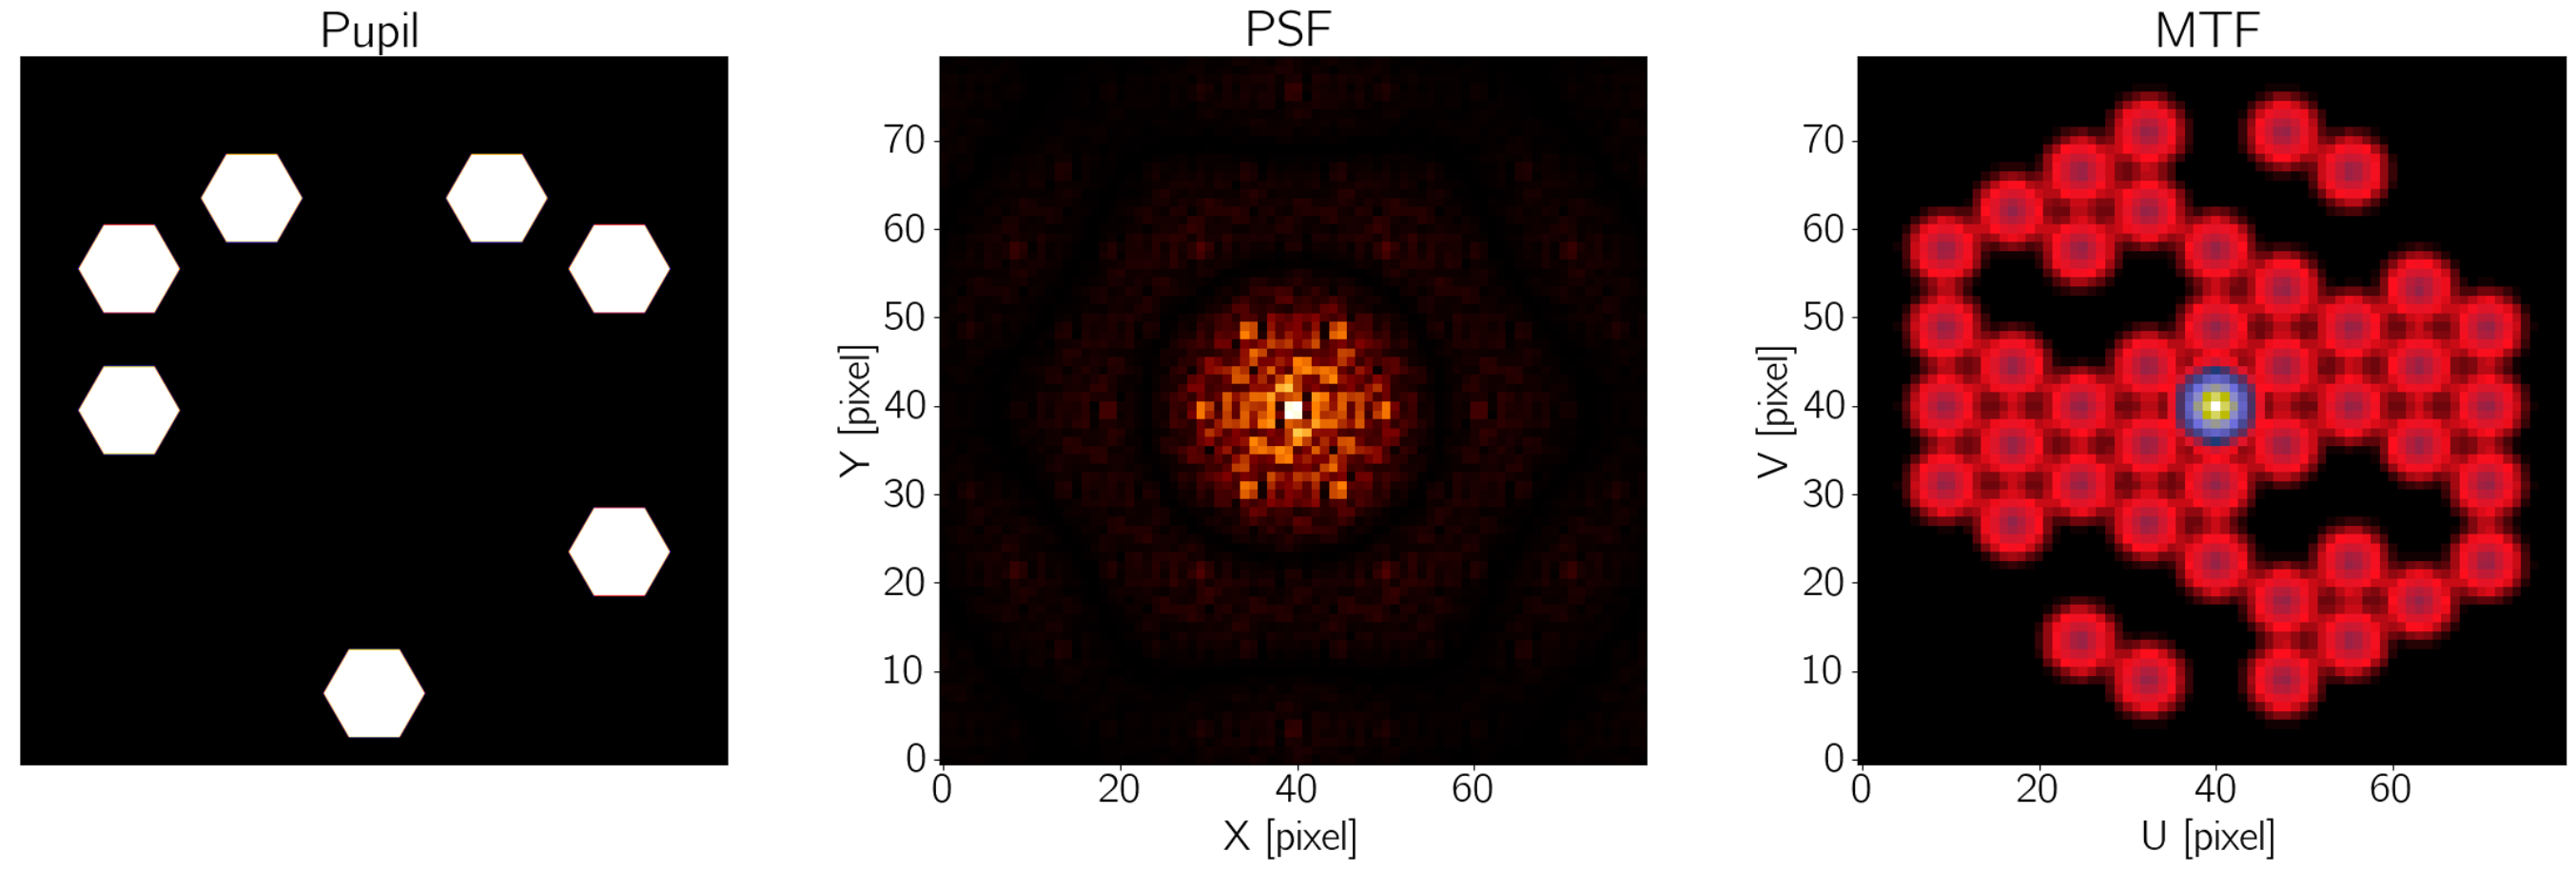
\includegraphics[width=\linewidth]{figures/analyse_niriss_ami.png}
    \end{center}
  }
  % \only<2>{
  %   First way to think about this: "high pass filter"
  %   \begin{center}
  %     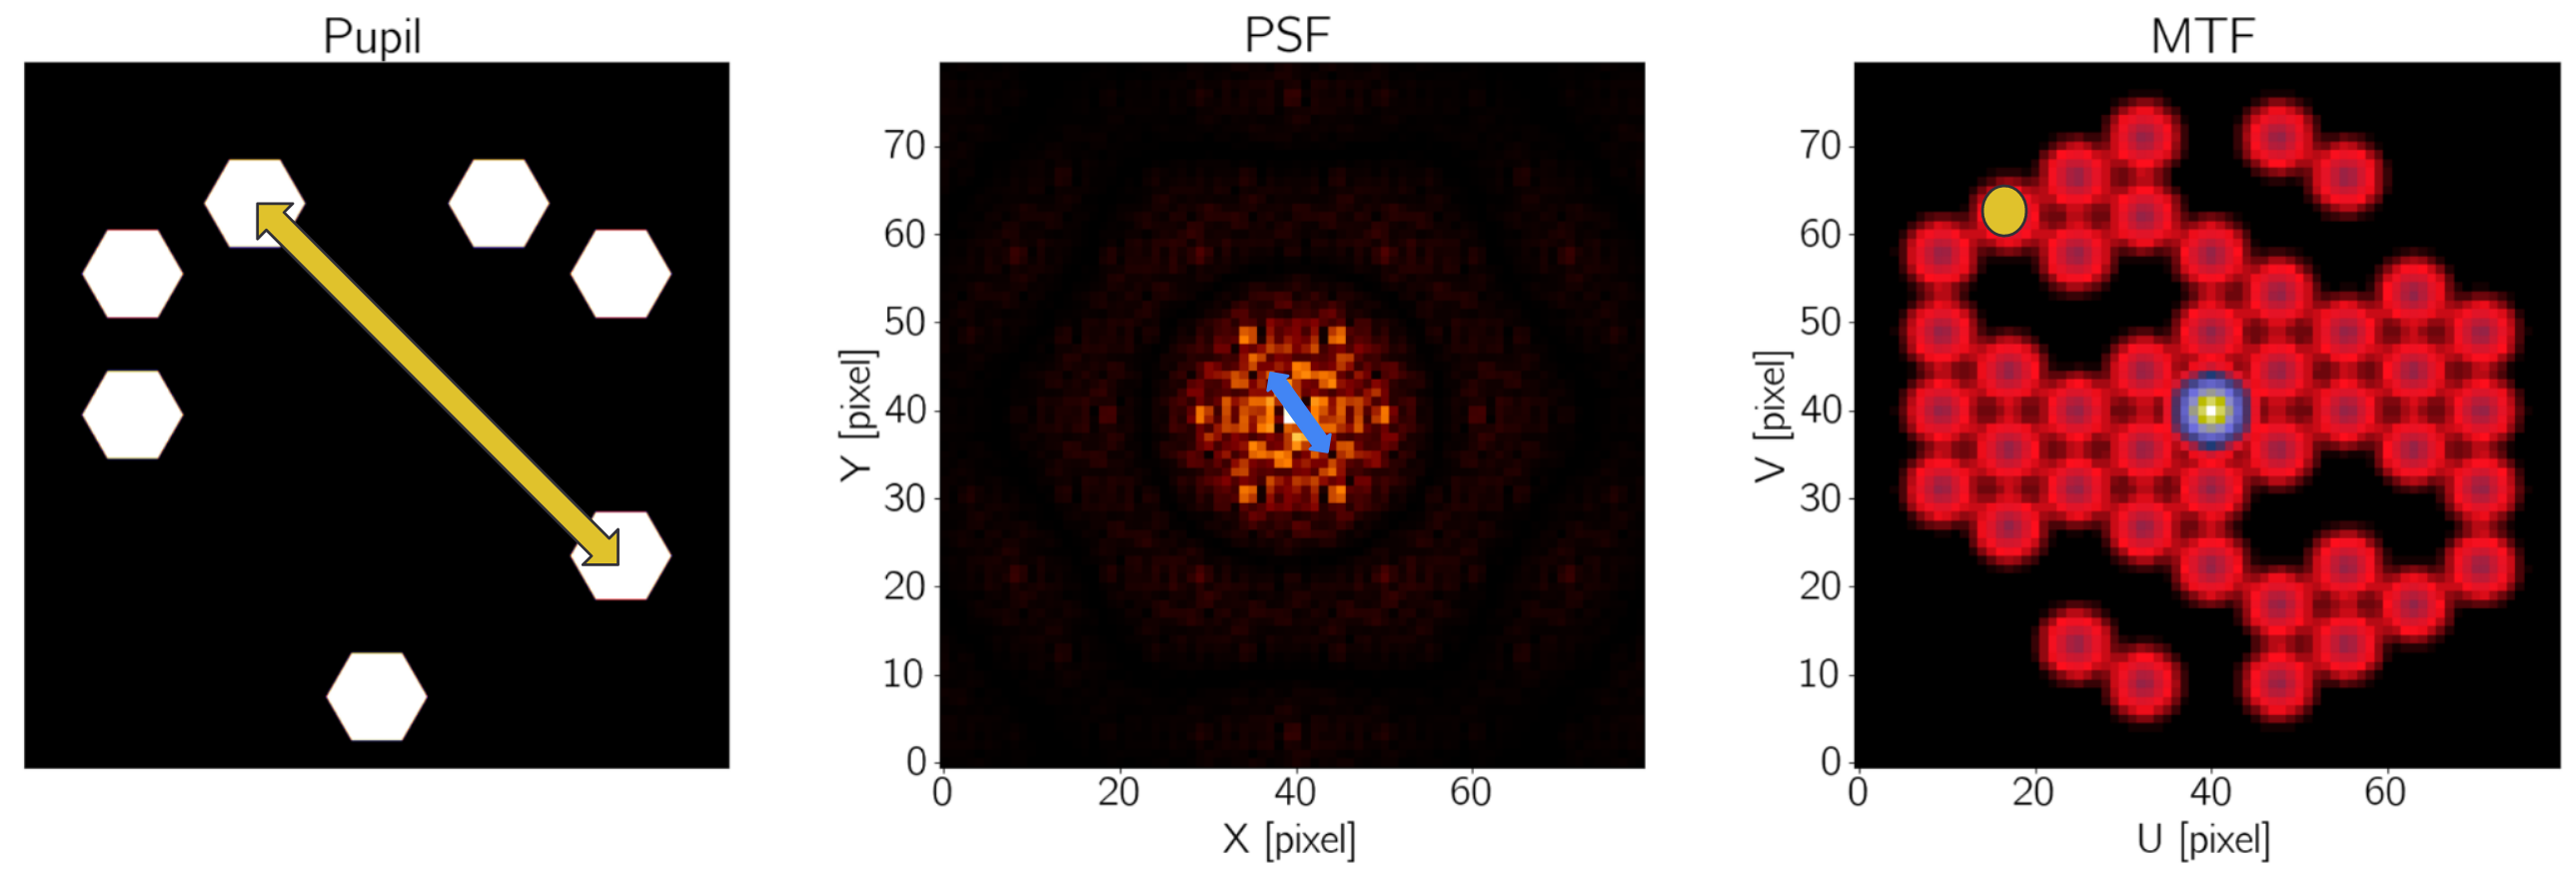
\includegraphics[width=\linewidth]{figures/ami_long_baseline.png}
  %   \end{center}
  % }
  % \only<3>{
  %   But most importantly: self-calibration
  %   \begin{center}
  %     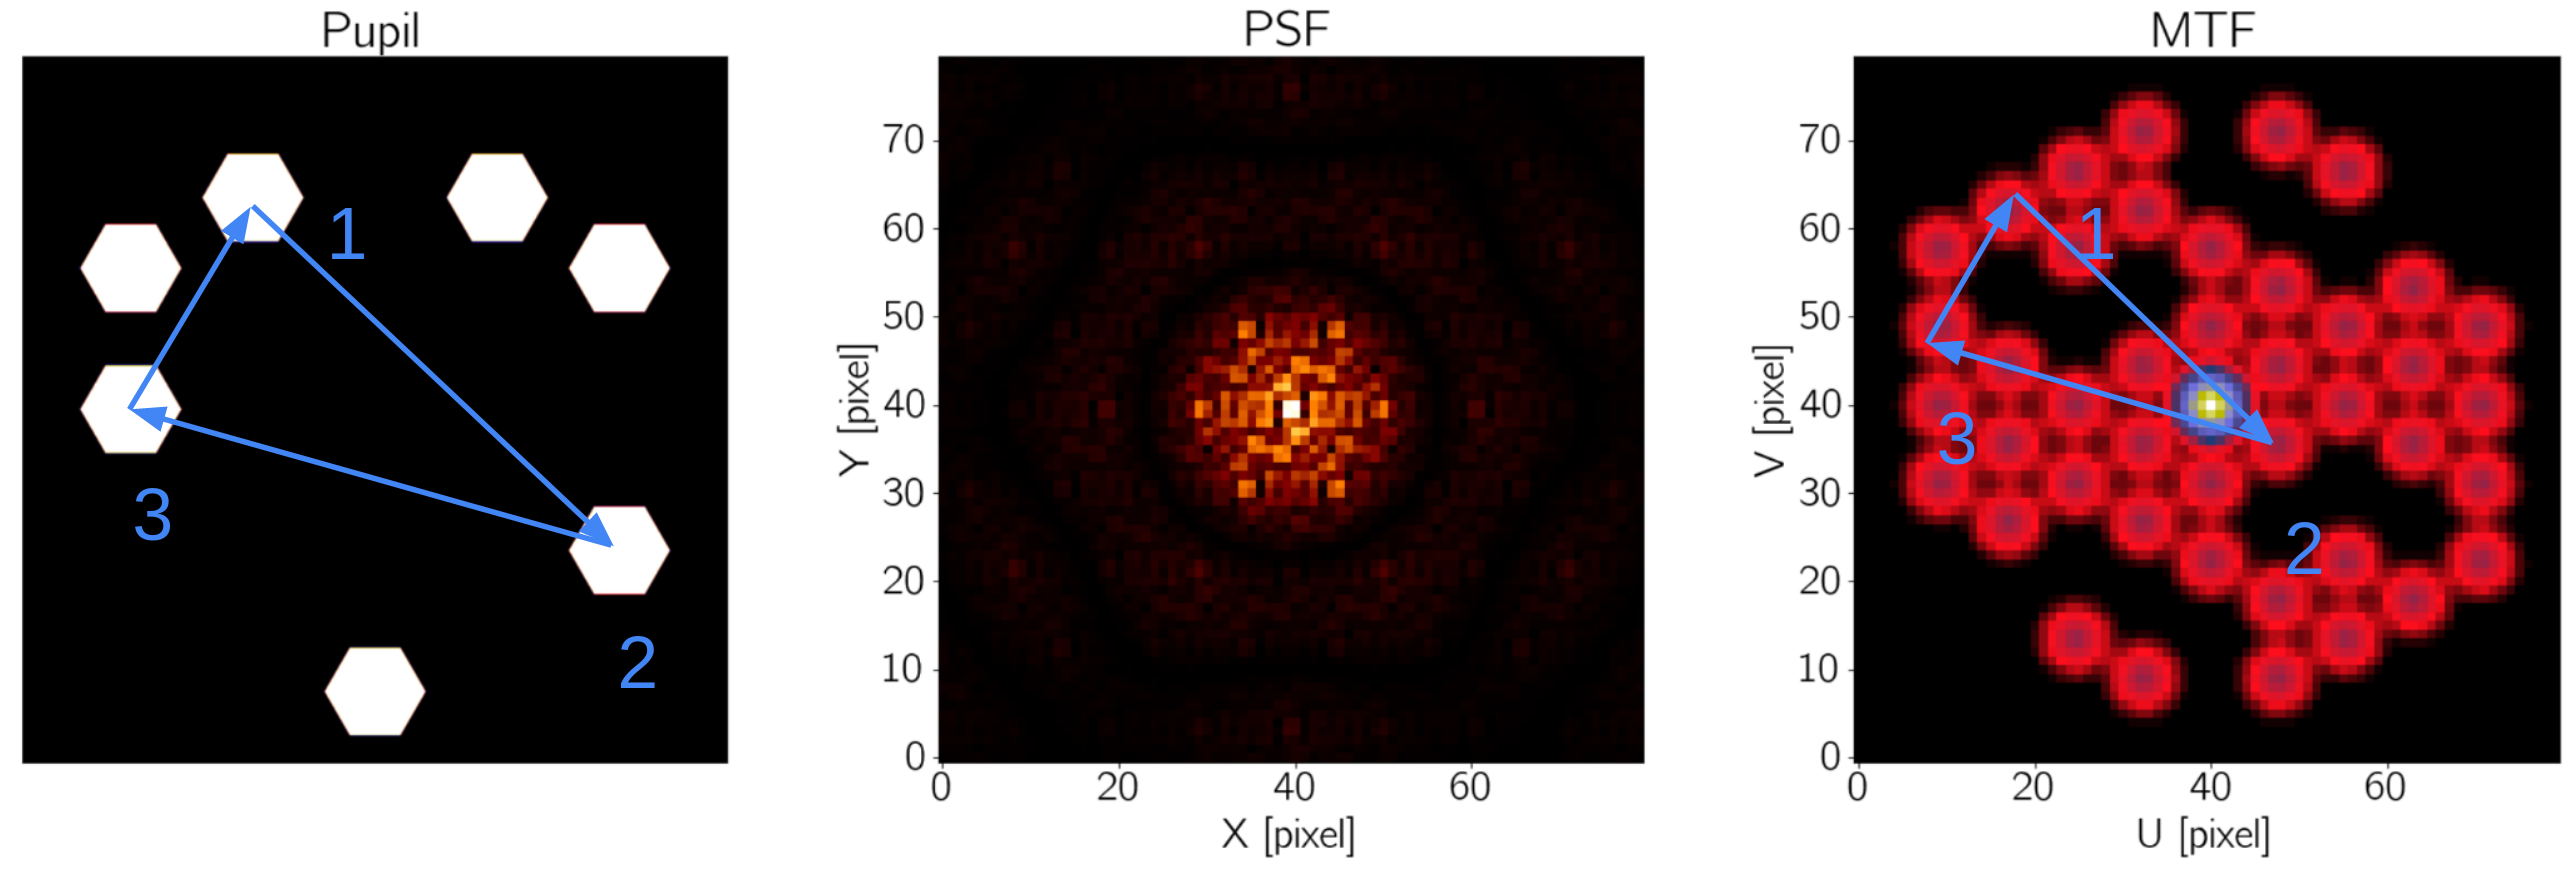
\includegraphics[width=\linewidth]{figures/ami_triagnle.png}
  %   \end{center}
  % }
\end{frame}

%% Can also apply to NRM Mask
\begin{frame}{Example binary}
  \begin{center}
    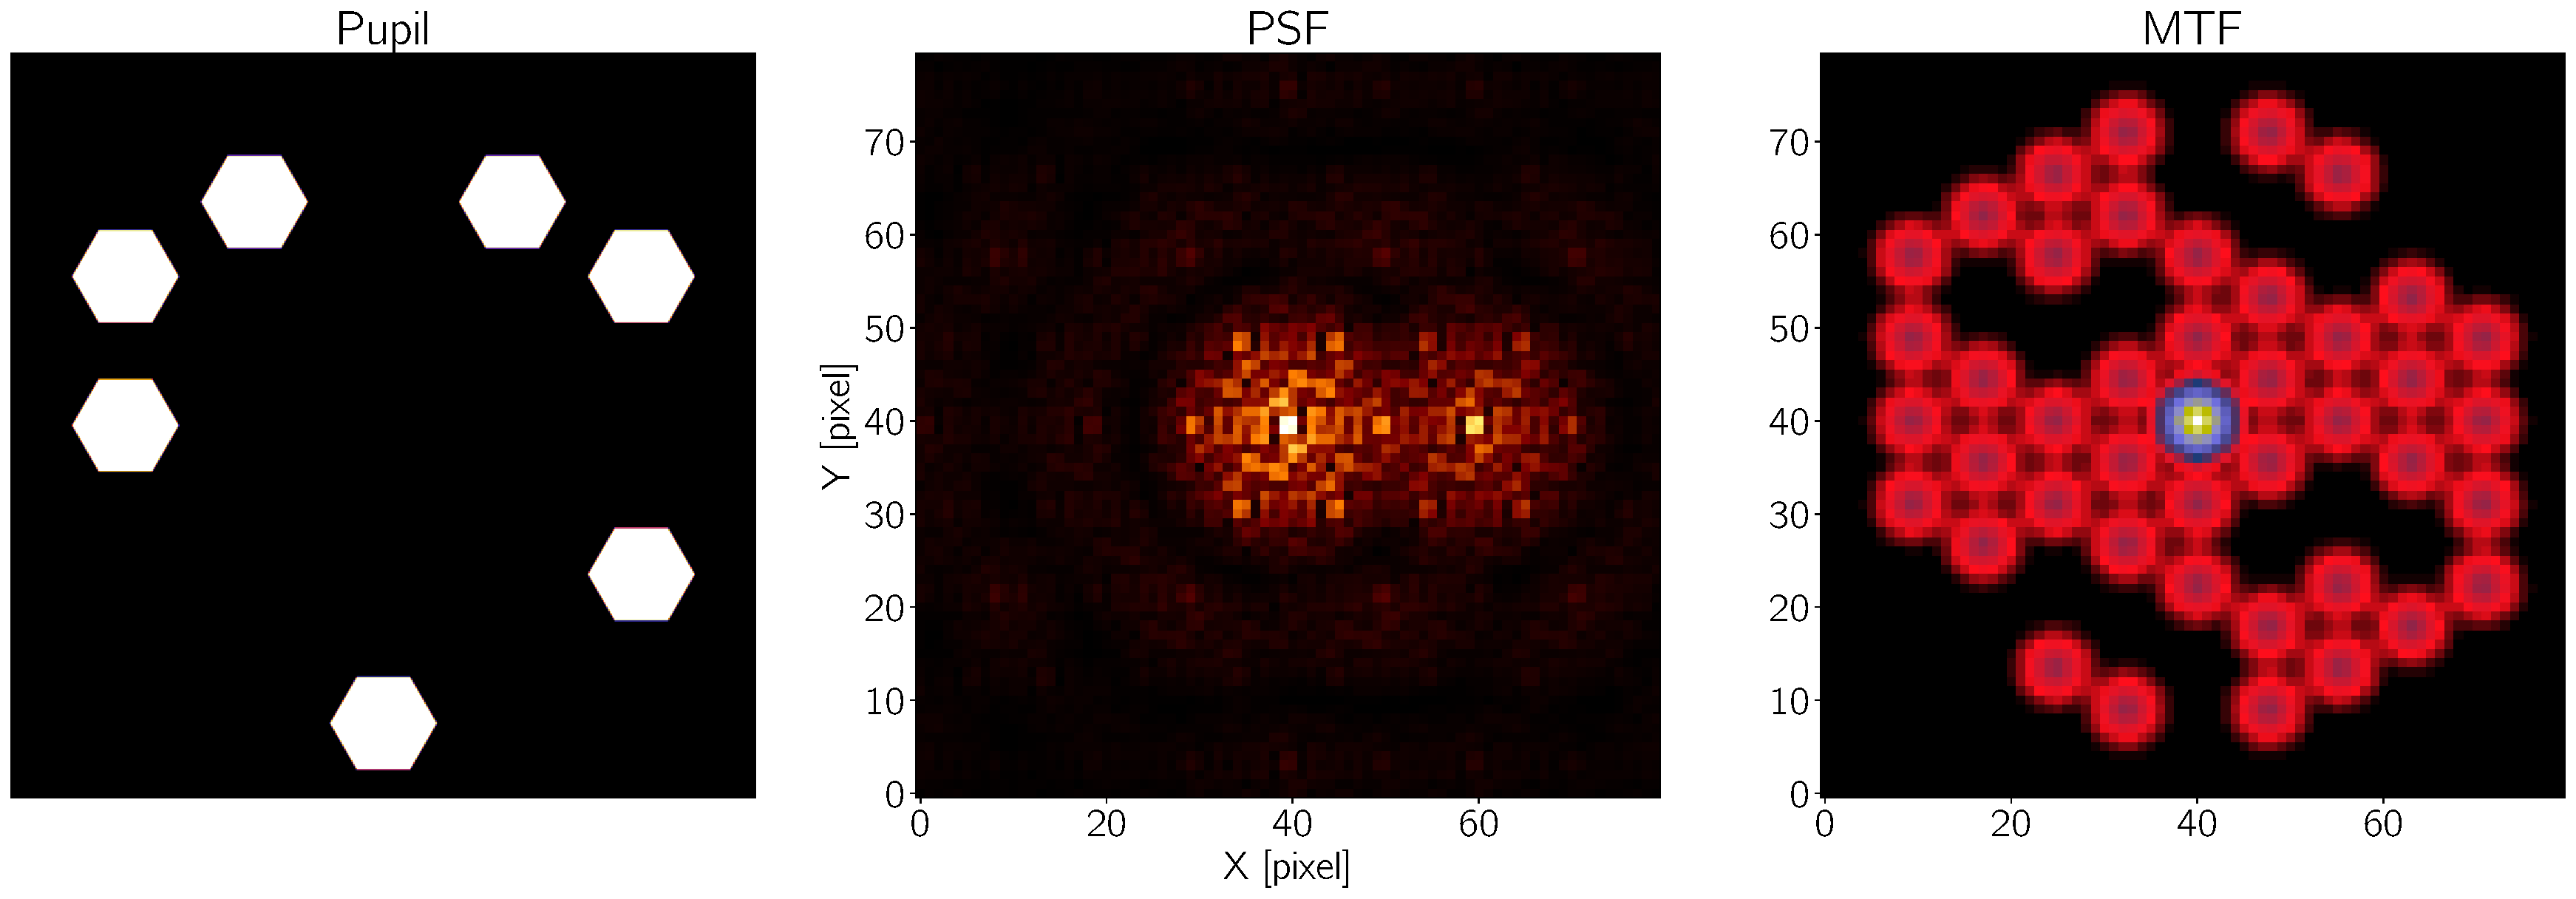
\includegraphics[width=\linewidth]{figures/analyse_niriss_ami_bin_sep_20_cr_0.5.pdf}
  \end{center}
\end{frame}
\begin{frame}{Same binary but closer}
%% Closer is harder
  \begin{center}
    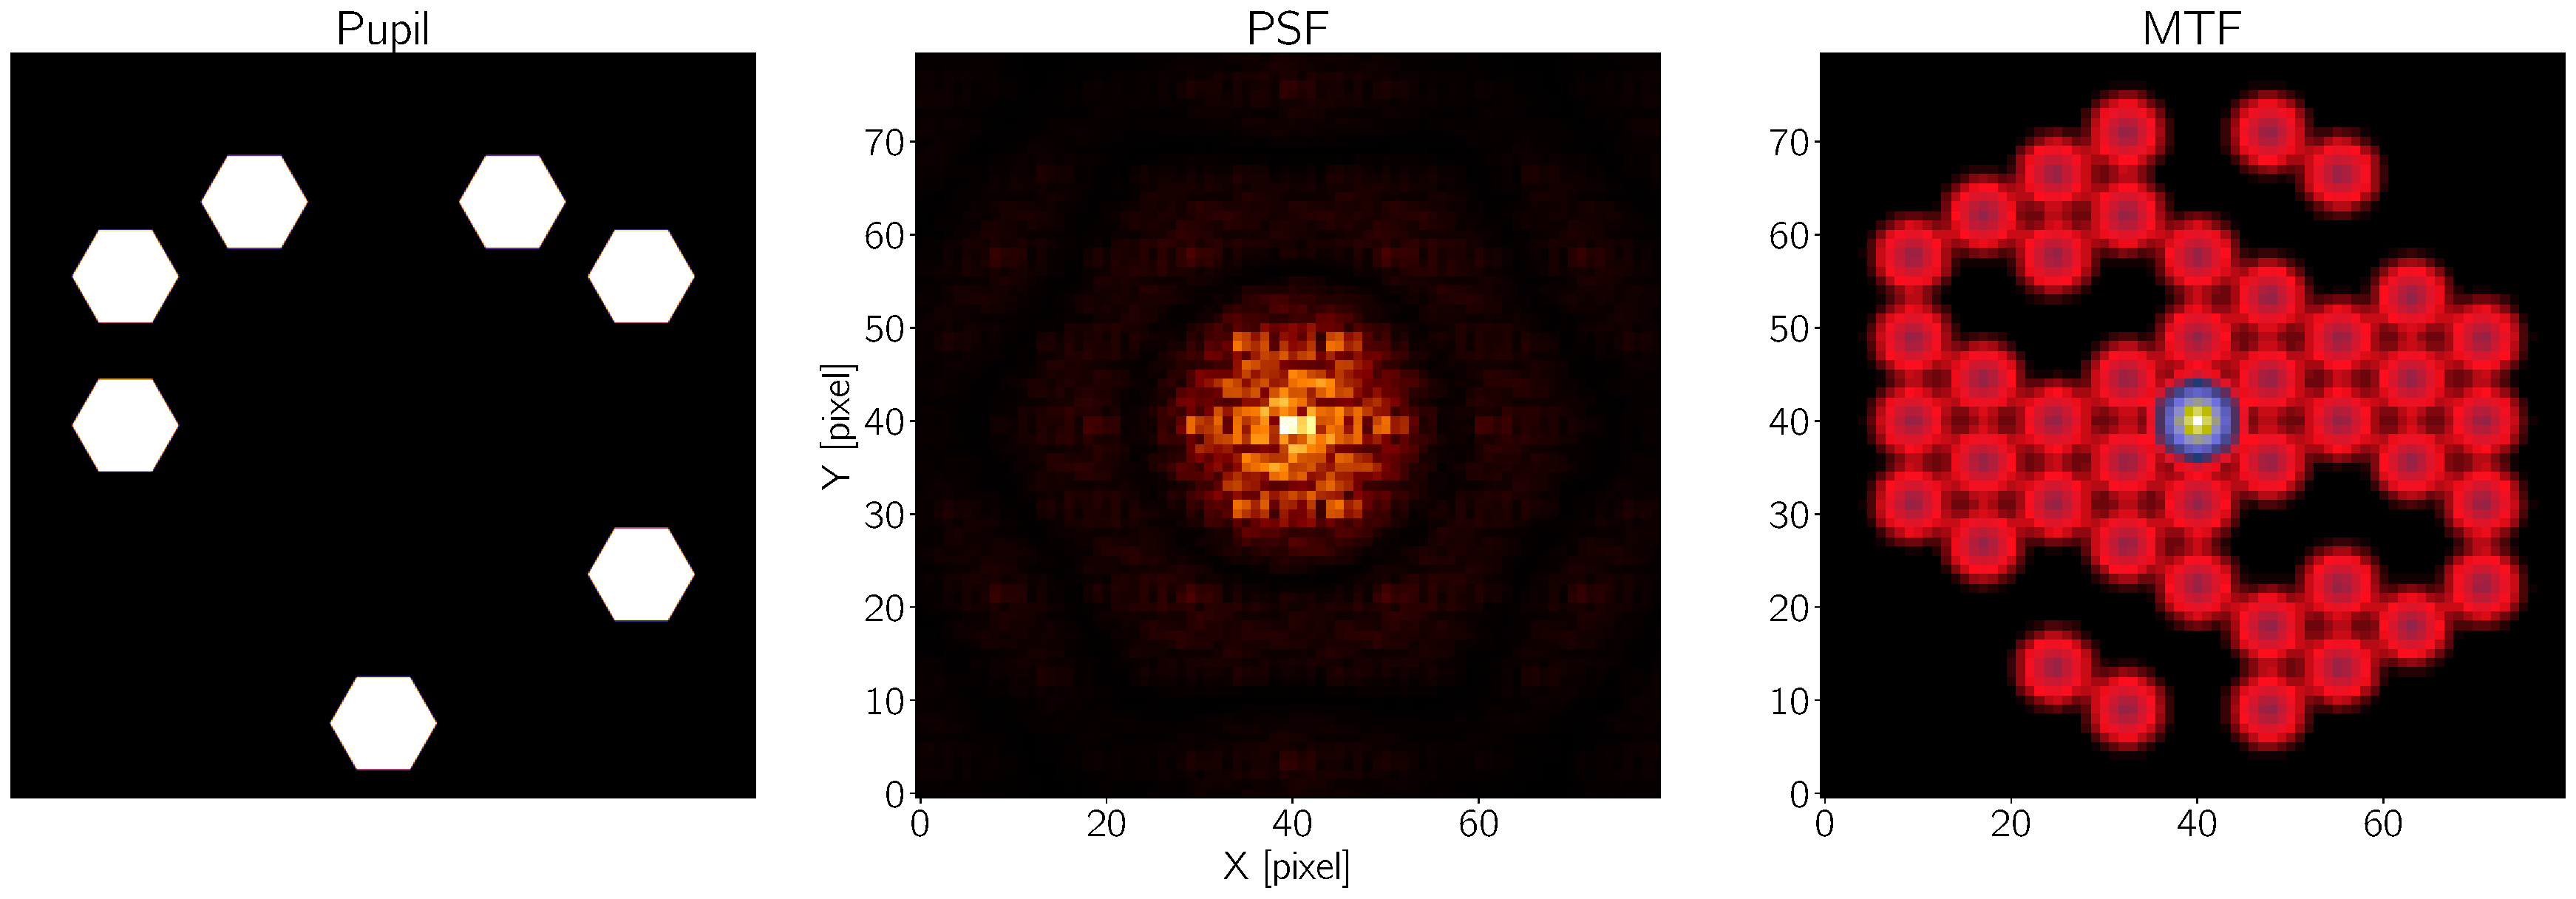
\includegraphics[width=\linewidth]{figures/analyse_niriss_ami_bin_sep_2_cr_0.5.pdf}
  \end{center}
\end{frame}
\begin{frame}{Giant planet}
  \begin{center}
    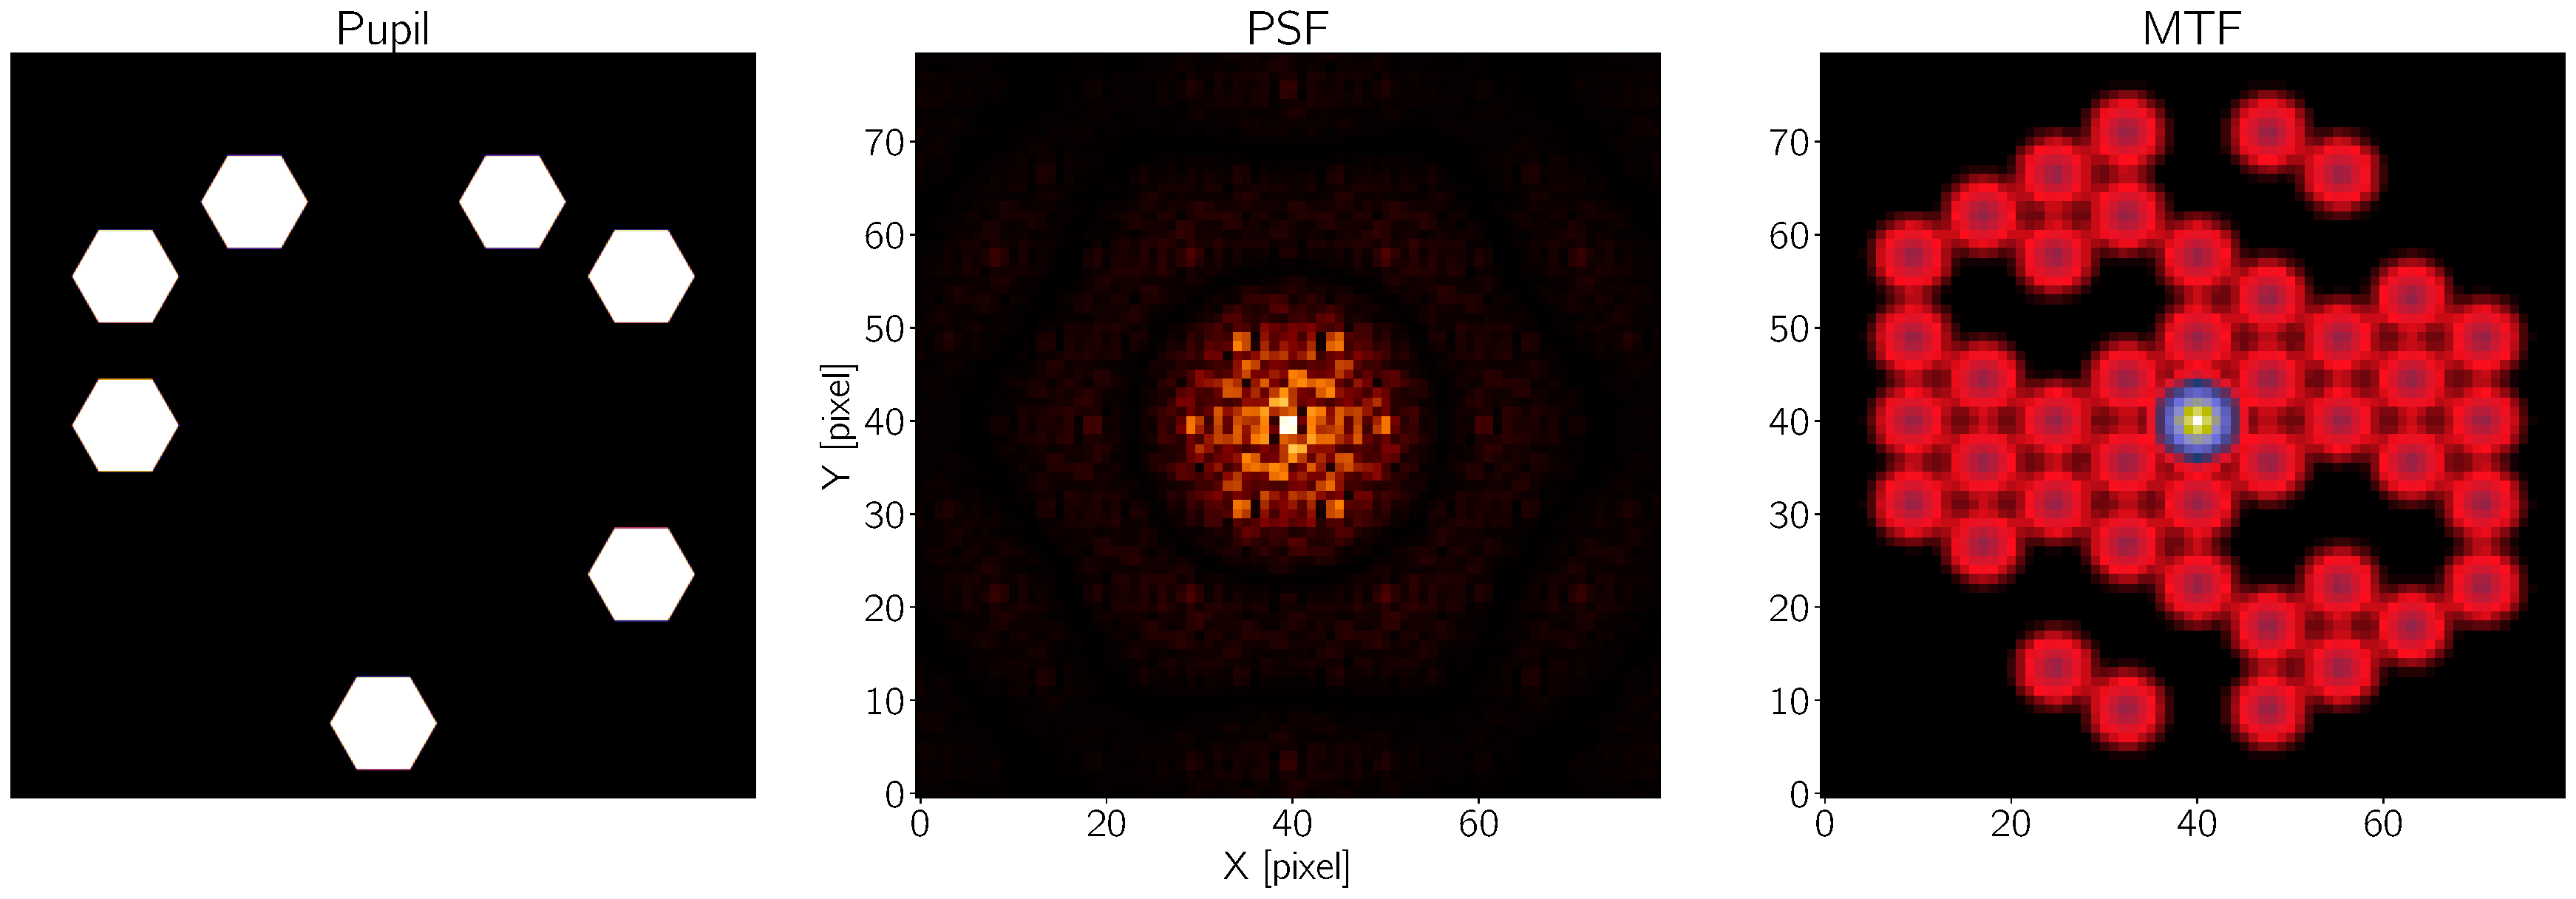
\includegraphics[width=\linewidth]{figures/analyse_niriss_ami_bin_sep_2_cr_0.0001.pdf}
  \end{center}
\end{frame}

% \begin{frame}{Searching for planets with AMI}
%   JWST/NIRISS GTO program, P.I. Julien Rameau:
%   \begin{wideitemize}
%     \item Search for giant planets around young, bright stars:
%       \begin{itemize}
%         \item HR 8799 (4 known planets $>$ 15 AU)
%         \item HD 95086 (known planet cannot explain gap in disk)
%         \item HD 115600 (ring-shaped disk)
%       \end{itemize}
%     \item Obtain luminosity measurements
%     \item Better understand planet formation
%     \item Will also be observed with NIRPS (high resolution spectroscopy)
%   \end{wideitemize}
% \end{frame}

\begin{frame}{Searching for planets with AMI}
  \begin{columns}
    \column{0.3\linewidth}
    \centering
    HR 8799

    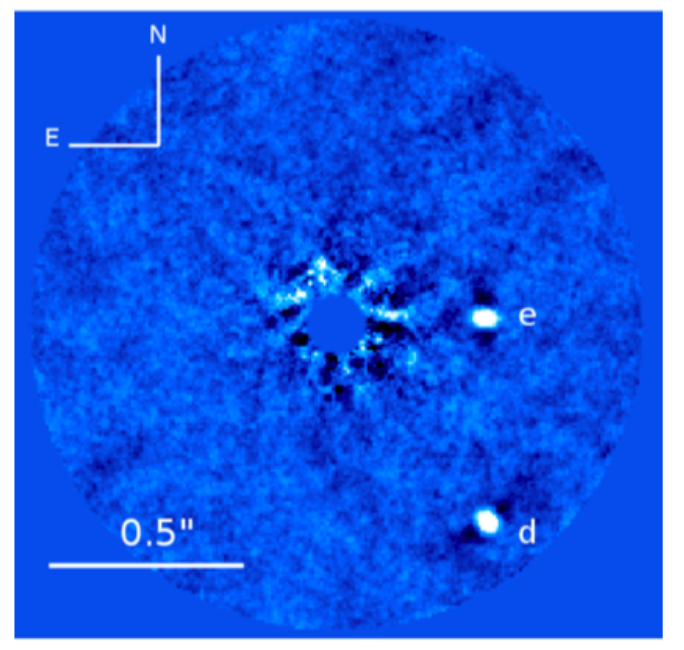
\includegraphics[width=\textwidth]{figures/hr8799_image.png}
    \column{0.3\linewidth}
    \centering
    HD 95086

    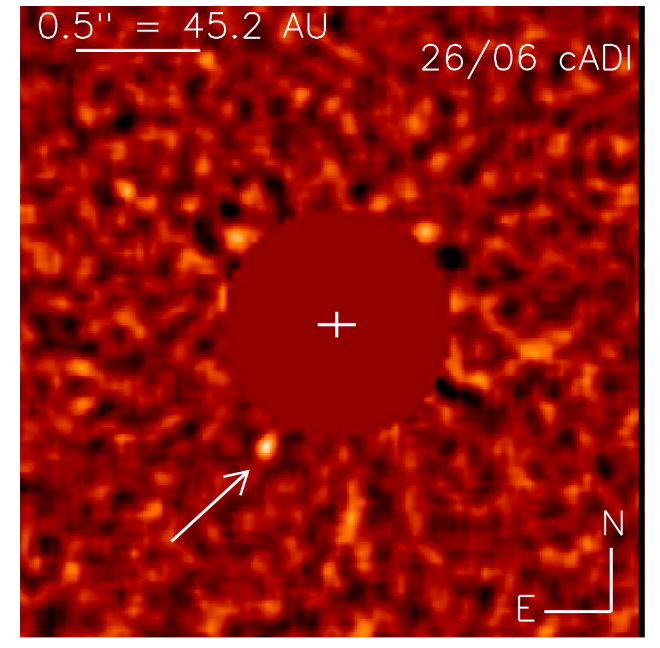
\includegraphics[width=\textwidth]{figures/hd95086_image.png}
    \column{0.33\linewidth}
    \centering
    HD 115600

    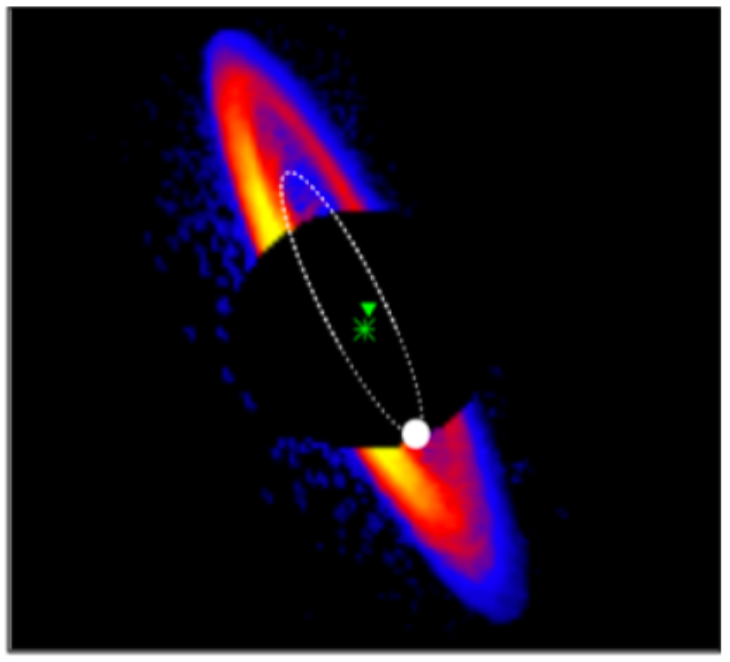
\includegraphics[width=\textwidth]{figures/hd115600.png}
  \end{columns}

  \footnotesize Figures: Zurlo et al. 2016, Rameau et al. 2013, Currie et al. 2015
\end{frame}

\begin{frame}{Searching for planets with AMI: HD 95086}
  \begin{wideitemize}
    \item 1 known planet (55 AU)
    \item Gap in debris disk $\rightarrow$ 1-3 additional planets?
    % \item Observed summer 2023
  \end{wideitemize}
  \begin{center}
    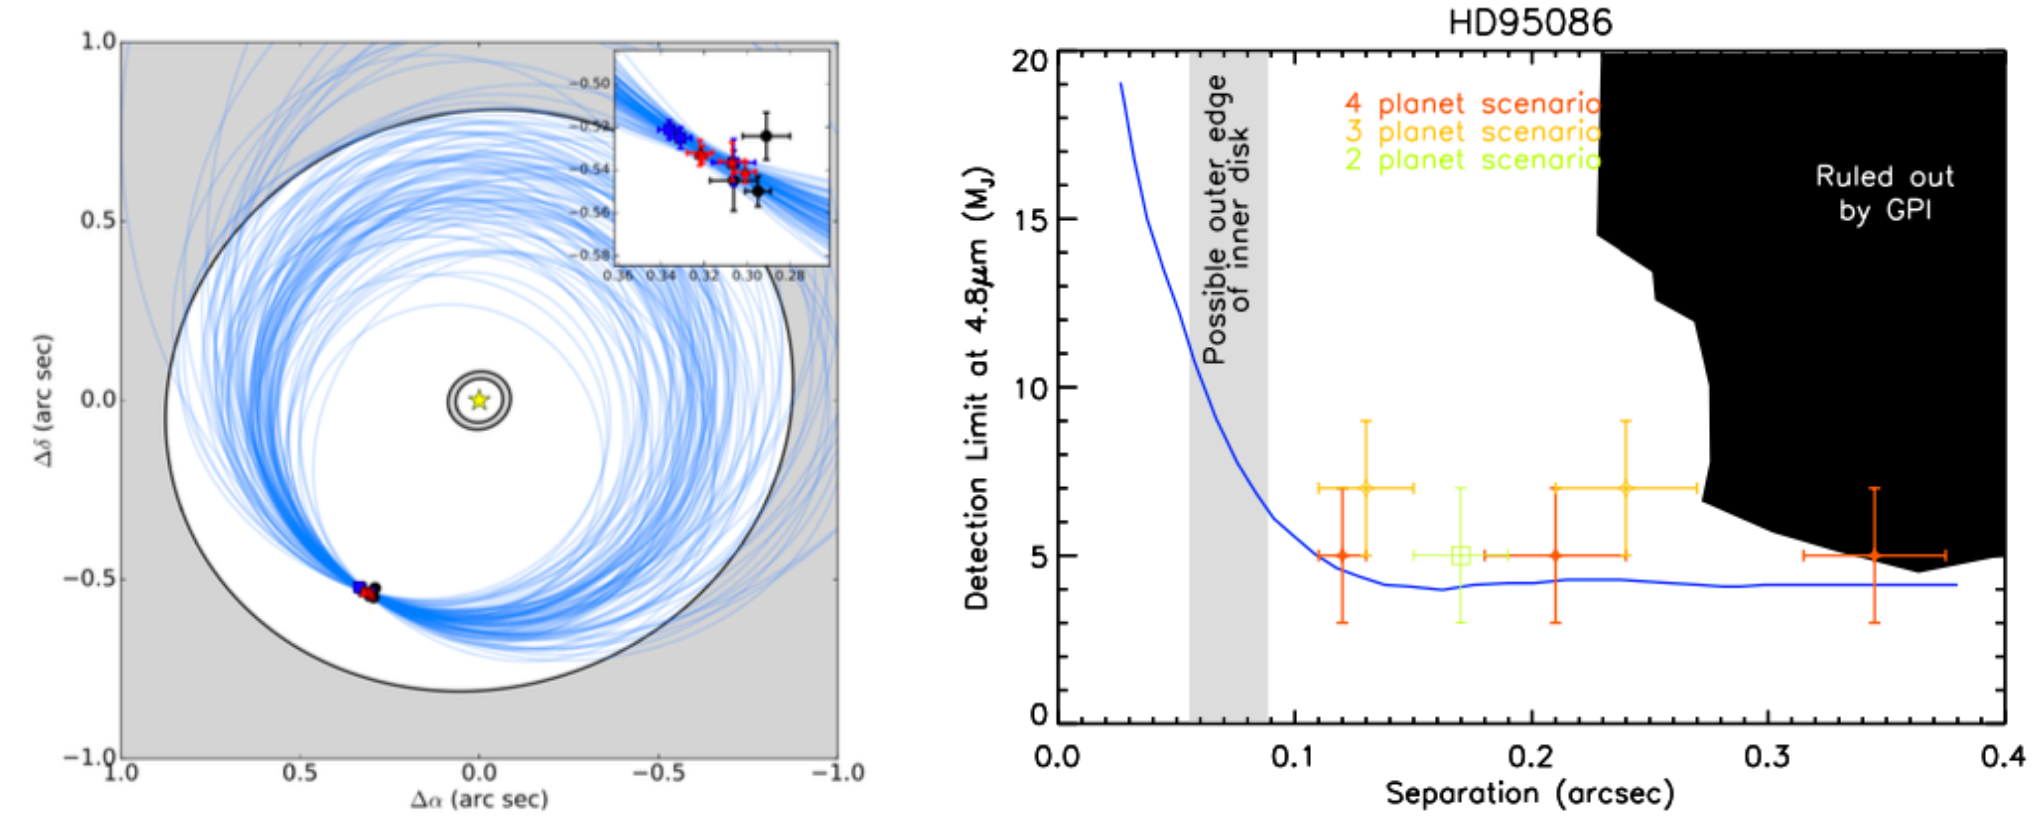
\includegraphics[width=\linewidth]{figures/hd95086_contrast.png}
  \end{center}

  \footnotesize Figures: J. Rameau
\end{frame}

% \begin{frame}{Searching for planets with AMI: HR 8799}
%   \begin{wideitemize}
%     \item 4 known planets (15-70 AU)
%     \item Inner HR 8799 f ?
%     % \item Observed summer 2023
%   \end{wideitemize}
%   \begin{center}
%     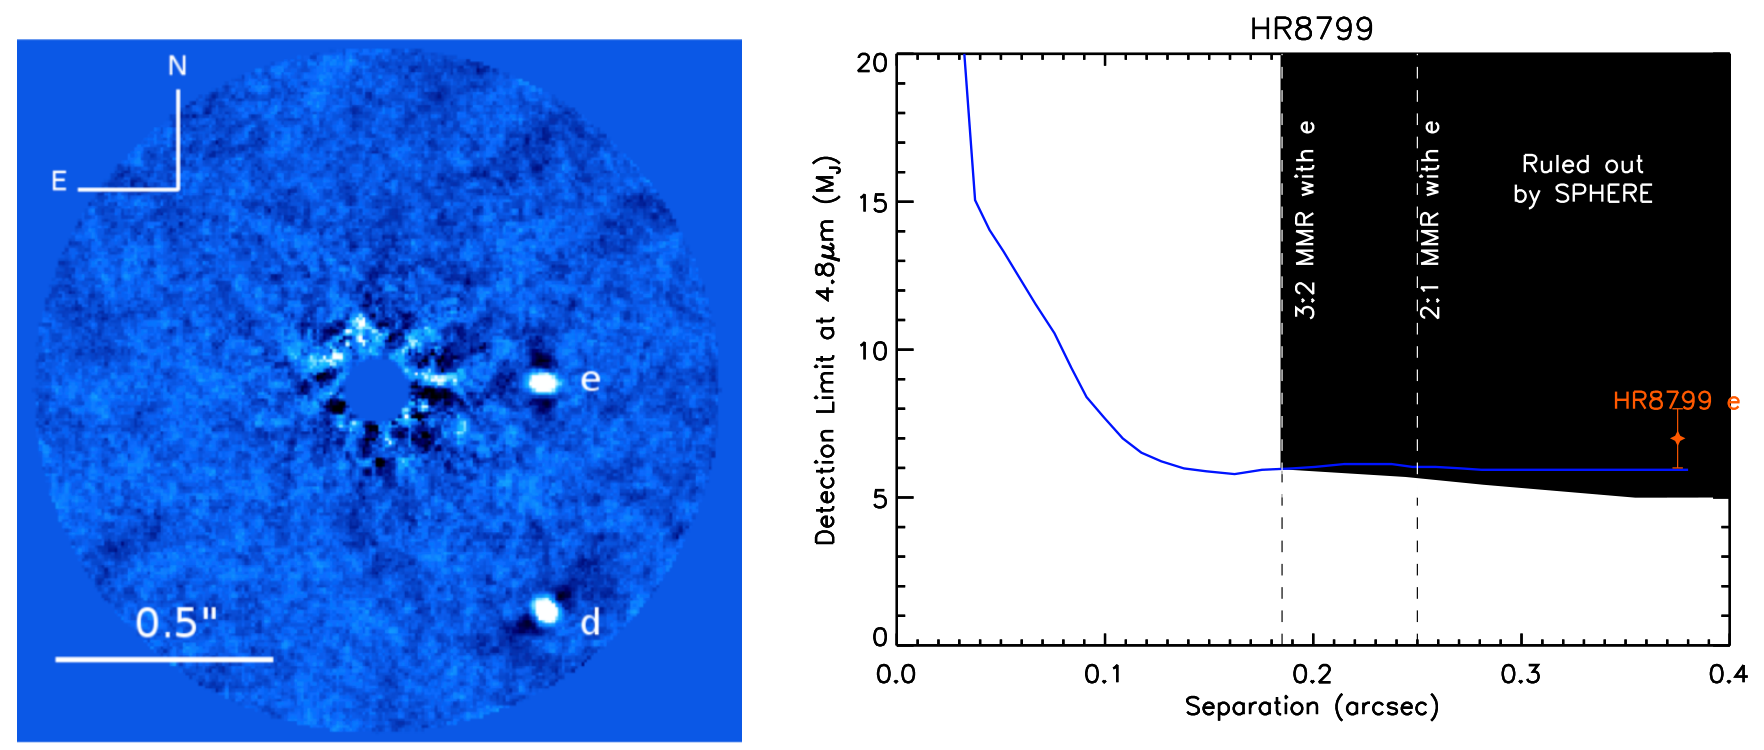
\includegraphics[width=\linewidth]{figures/hr8799_contrast.png}
%   \end{center}
%
%   \footnotesize Figures: Zurlo et al. 2016, J. Rameau
% \end{frame}

% \begin{frame}{Searching for planets with AMI: HD 115600}
%   \begin{wideitemize}
%     \item Ring-shaped debris disk $\rightarrow$ planet(s)?
%     \item Inclination (80 deg) does not favor ground-based detections
%     % \item Observed summer 2023
%   \end{wideitemize}
%   \begin{center}
%     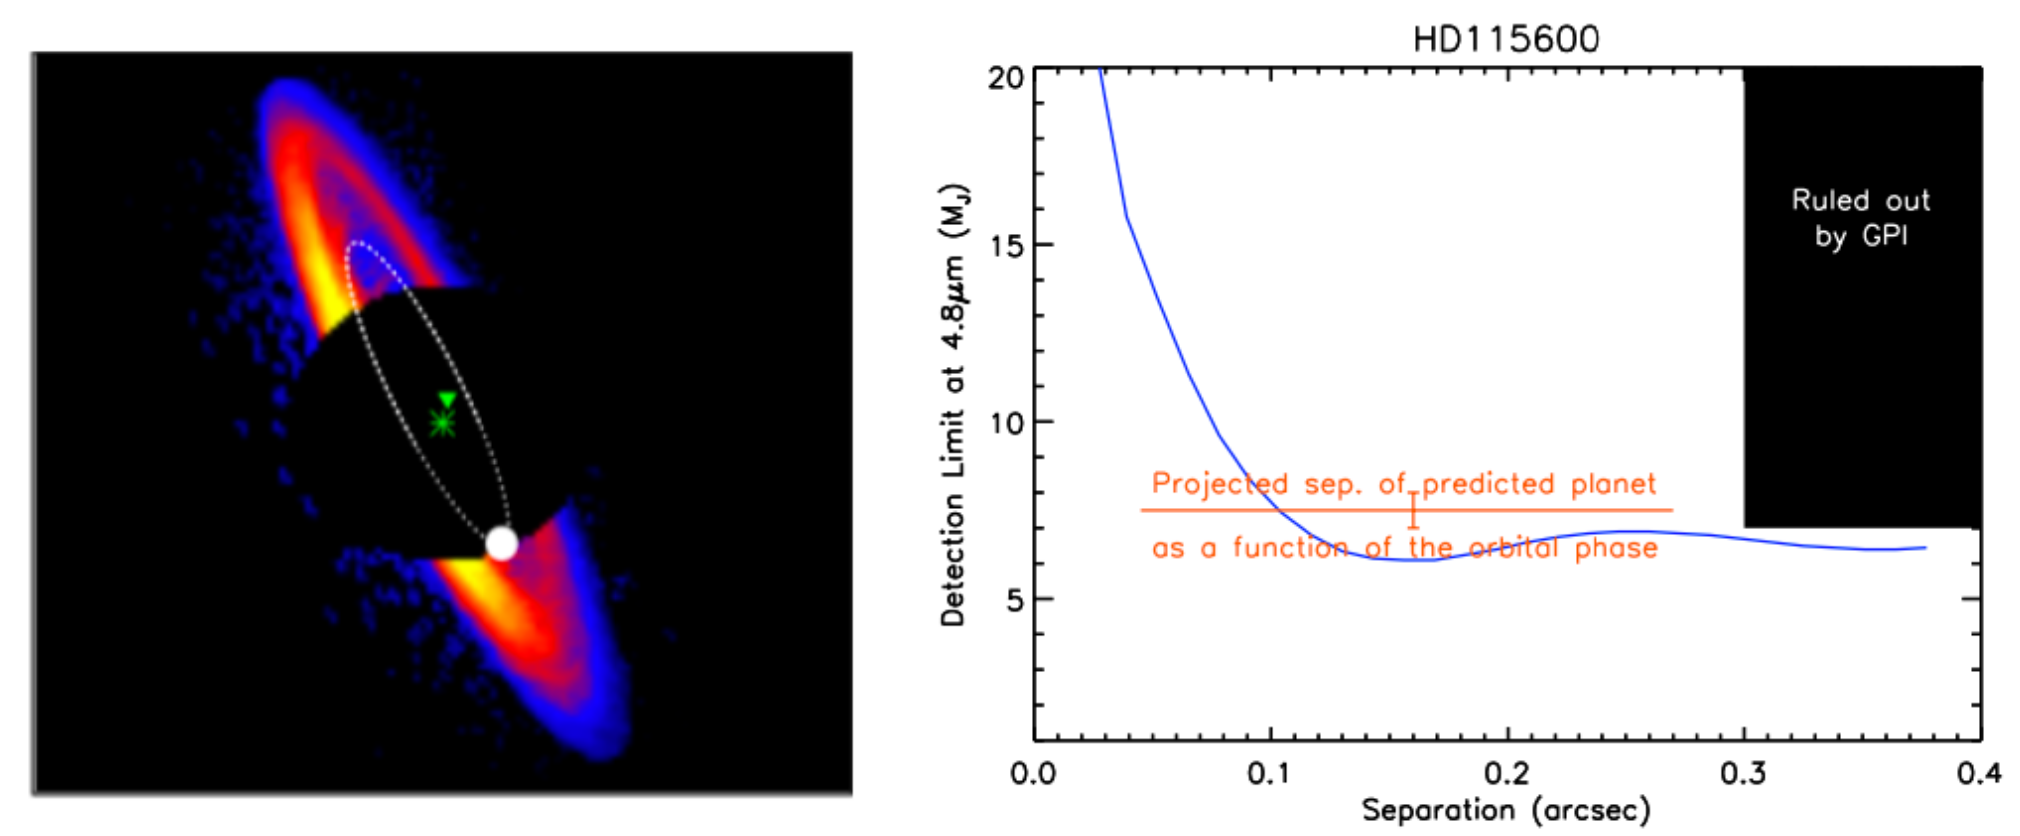
\includegraphics[width=\linewidth]{figures/hd115600_contrast.png}
%   \end{center}
%
%   \footnotesize Figures: Zurlo et al. 2016, J. Rameau
%   \footnotesize Figures: Currie et al. 2015, J. Rameau
% \end{frame}

\begin{frame}{What about faint objects?}
  \begin{center}
    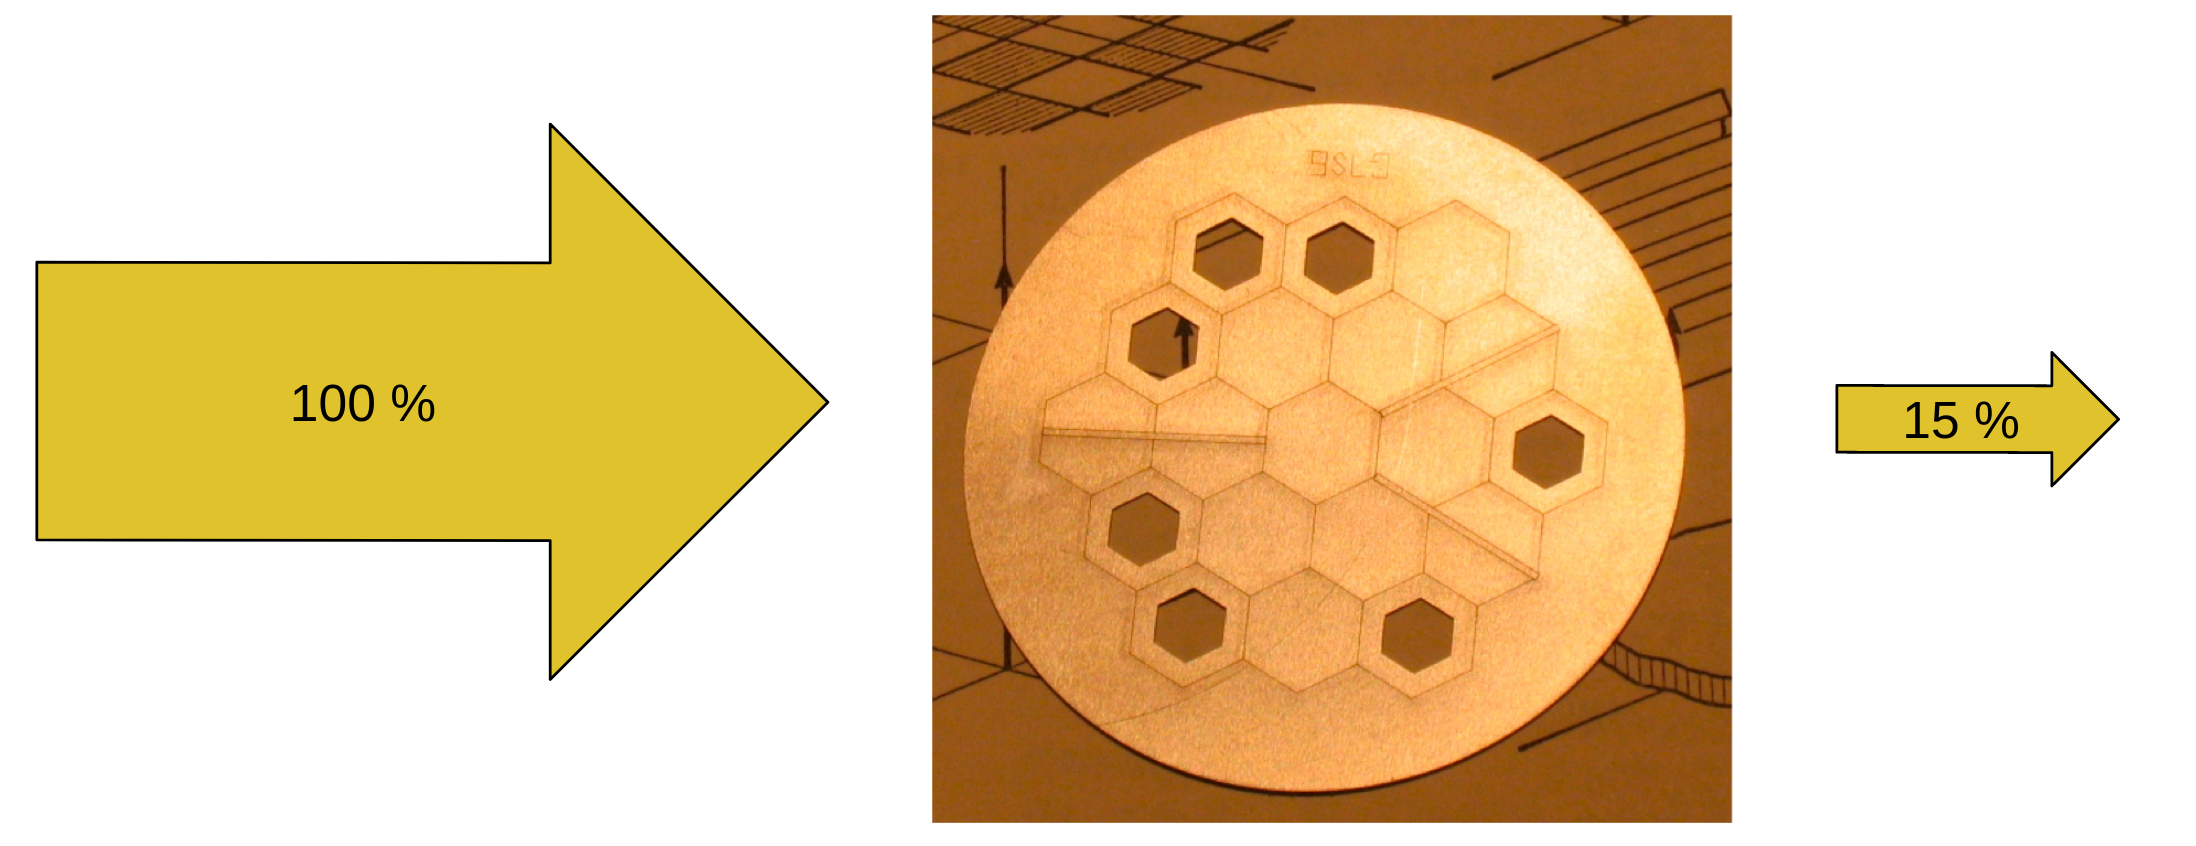
\includegraphics[width=\linewidth]{figures/mask_blocks_light.png}
  \end{center}
\end{frame}


% TODO: Building discrete rep of pupil and using interferometry techniques actually works too!

% TODO: Don't get rid of low freq info, but can self-calibrate observable and dtetect compaions

\begin{frame}{Kernel Phase}
  Approximate pupil as multiple sub-apertures\\ $\rightarrow$ use interferometric analysis\\ $\rightarrow$ observe faint objects with full pupil
  \begin{center}
    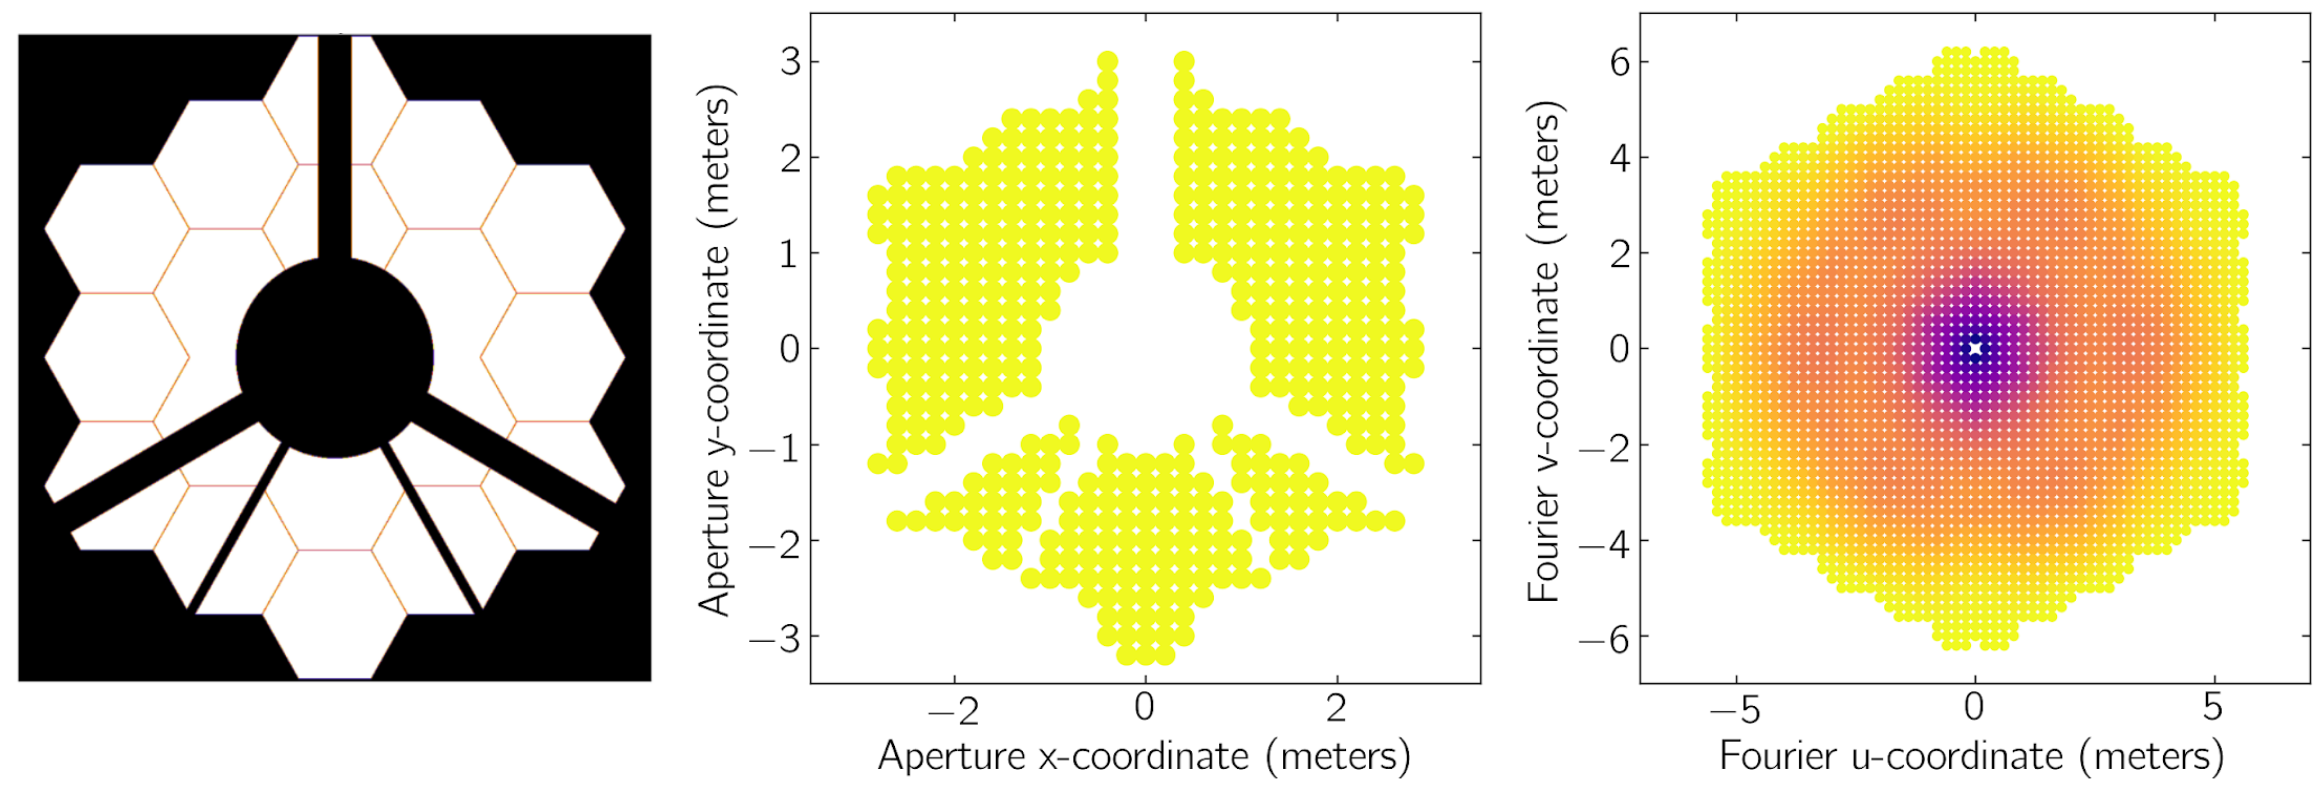
\includegraphics[width=\linewidth]{figures/kernel_model.png}
  \end{center}
\end{frame}

\begin{frame}{Searching for companions around Y dwarfs with kernel phase}


\begin{columns}
\column{0.4\textwidth}
  \begin{itemize}
    \item Companions?
    \item Giant planet?
    \item Study population and formation
    \item Could image coldest substellar objects to date
    % \item Determine companion frequency and mass-ratio distribution.
    % \item Probe low mass (q ~ 0.1) and short separation ($<$ 1 AU)
    % \item Peak at 4 $\mu$m $\rightarrow$ Can't be done from ground
  \end{itemize}
\column{0.6\textwidth}
  \begin{center}
    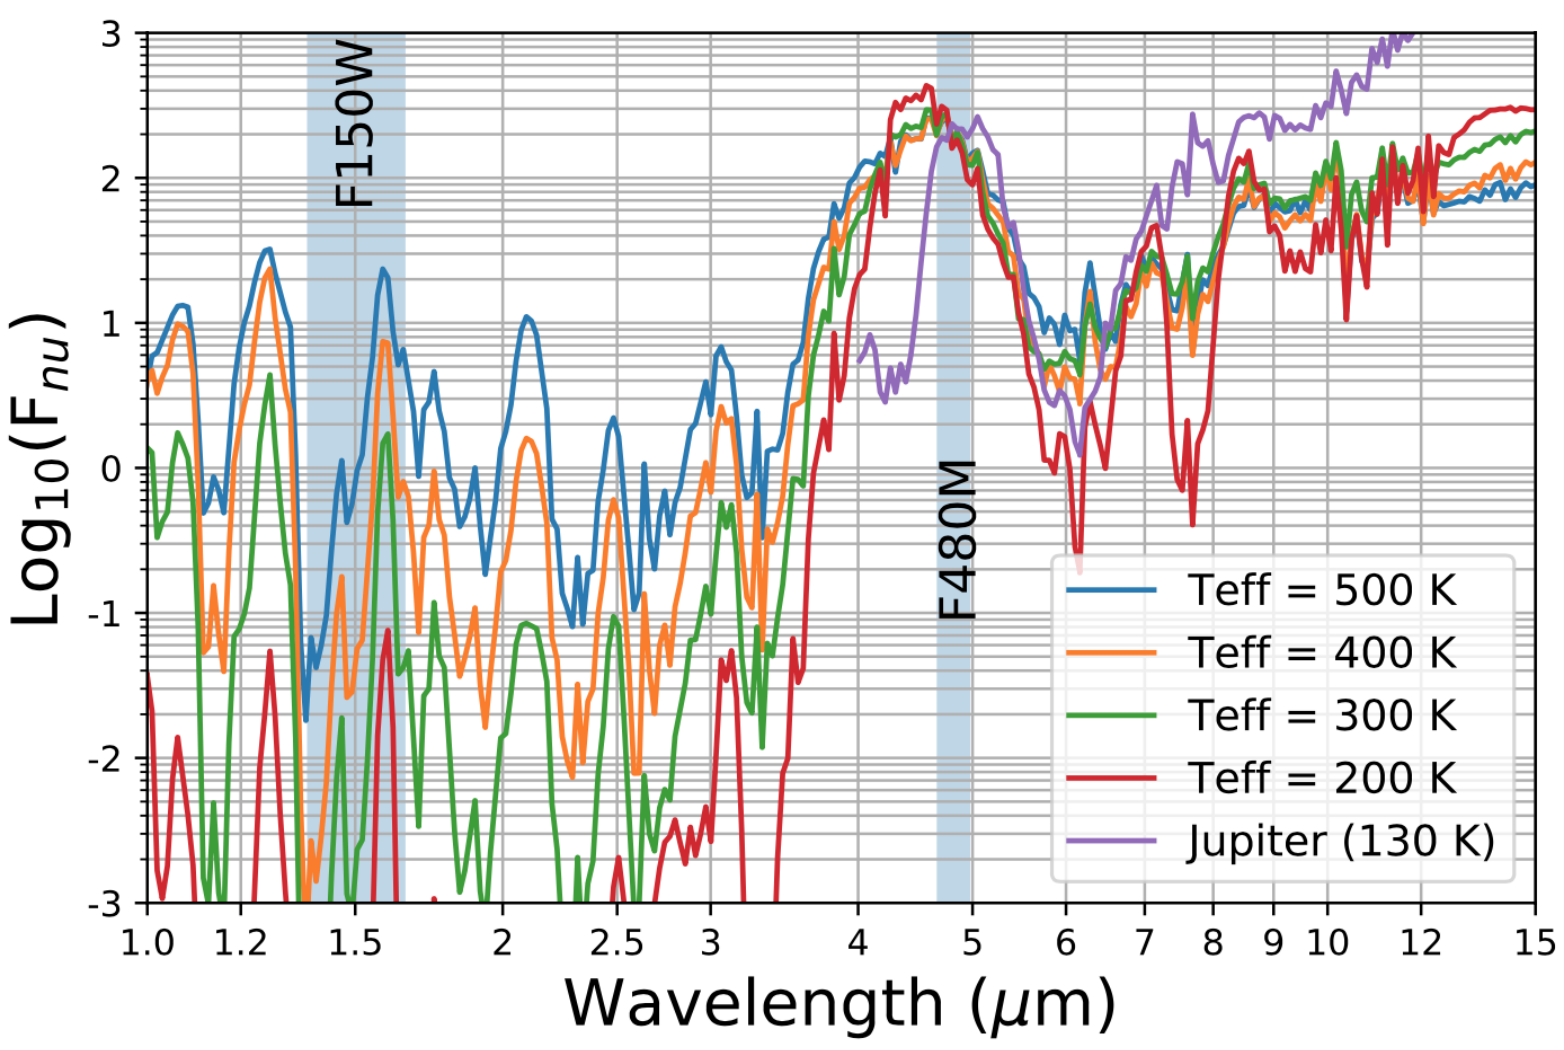
\includegraphics[width=\linewidth]{figures/bd_spectra.png}
  \end{center}
\end{columns}
\end{frame}

% \begin{frame}{Searching for companions around Y dwarfs with kernel phase}
%   JWST/NIRCam GO program led by Loïc Albert:
%   \begin{wideitemize}
%     \item 20 of the coldest ($<$ 500 K) and least massive (5-30 M$_\text{jup}$) brown dwarfs
%     \item Can they support companions? Giant planet?
%     \item Determine companion frequency and mass-ratio distribution.
%     \item Probe low mass (q $\sim$ 0.1) and short separation ($<$ 1 AU)
%     \item Peak at 4 $\mu$m $\rightarrow$ Can't be done from ground
%     \item Could image coldest substellar objects to date
%   \end{wideitemize}
%   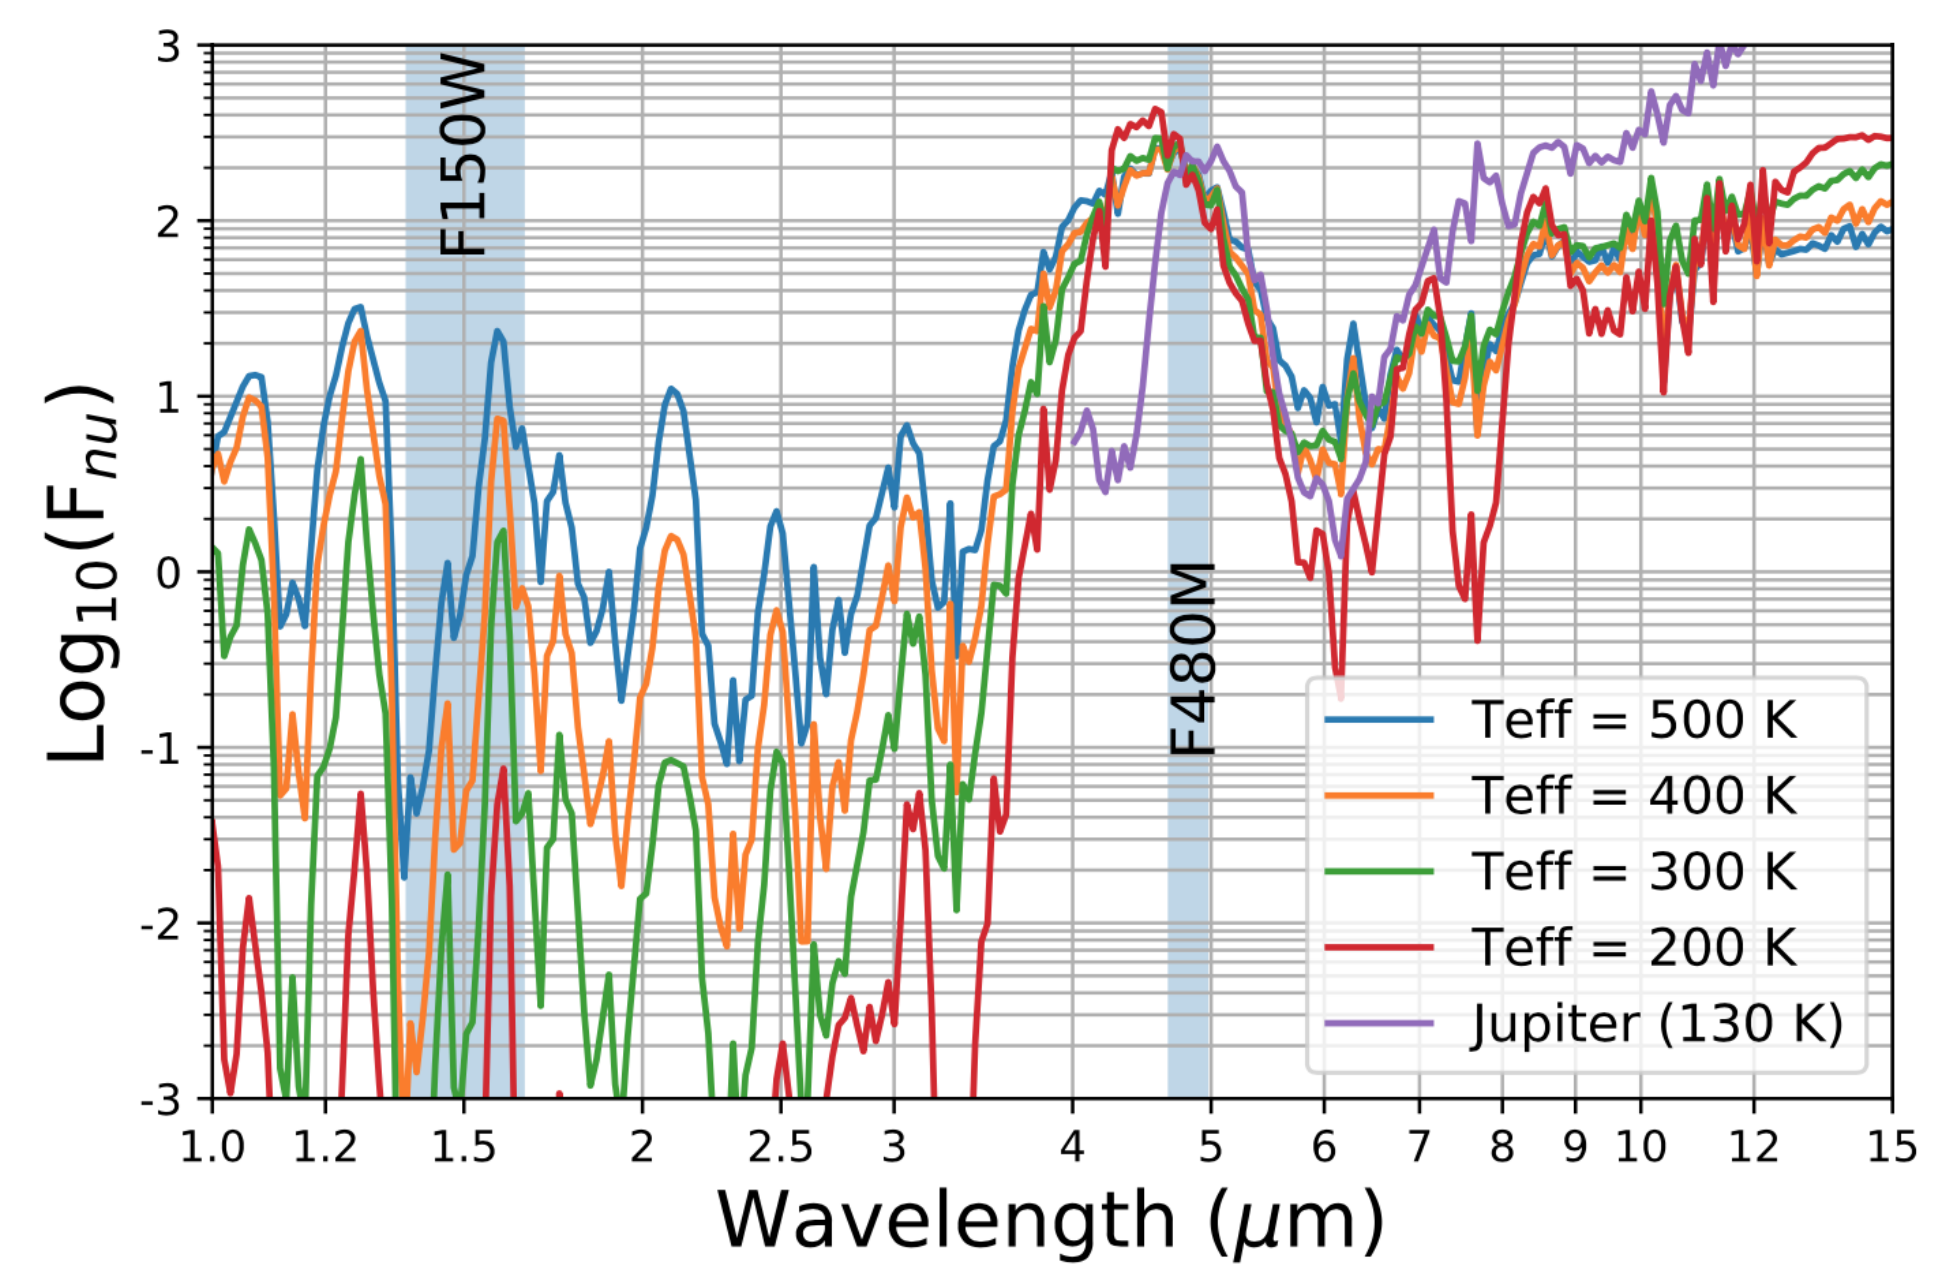
\includegraphics[width=0.8\linewidth]{figures/y_dwarf_spectra.png}
% \end{frame}

\begin{frame}{Summary}
  \begin{wideitemize}
    \item NIRISS AMI: observe bright stars to directly detect companions
    \item Kernel phase: use full pupil to search for companions around faint targets
    \item Next steps
    \begin{itemize}
      \item Updated simulations
      \item Test updated pipelines (image plane and Fourier plane)
      \item Bayesian model comparison (disk, multiple planets)
      \item Image reconstruction?
    \end{itemize}
  \end{wideitemize}
\end{frame}

% \begin{frame}{Kernel Phase}
%
%   Now all we need to do is find a matrix $\vect{K}$ that cancels $\vect{A}$ ($\vect{K}\cdot\vect{A} = \vect{0}$) to get rid of errors $\phi$
%
%   \begin{equation*}
%     \vect{K} \boldsymbol{\Phi} = \vect{K} \boldsymbol{\Phi}^O + \cancel{\vect{K} \vect{A} \cdot \vect{\phi}}
%   \end{equation*}
%
%   \onslide<2->{
%     This generic formulation is applicable to \textit{redundant} apertures (i.e. full pupil).
%   }
%
%   \onslide<3->{
%     One condition: high Strehl ratio (error for aperture $k$ can be approximated by $e^{i\phi_k} \approx 1 + i \phi_k)$
%   }
%
%   \onslide<4->{
%     $\vect{K}$ is the \textit{kernel} of $\vect{A}$ (math). Hence the name \textit{kernel phase}.
%   }
%
%   %% Generalization of inverse to non-diagonal matrices
%   \onslide<5->{
%     $\vect{K}$ is found by singular value decomposition (SVD)
%   }
%
% \end{frame}
%
% %% Instead of aperture mask, approximate pupil as many finite apertures
% \begin{frame}{Discrete pupil model}
%
%   Approximate pupil as many finite sub-apertures
%
%   \begin{center}
%     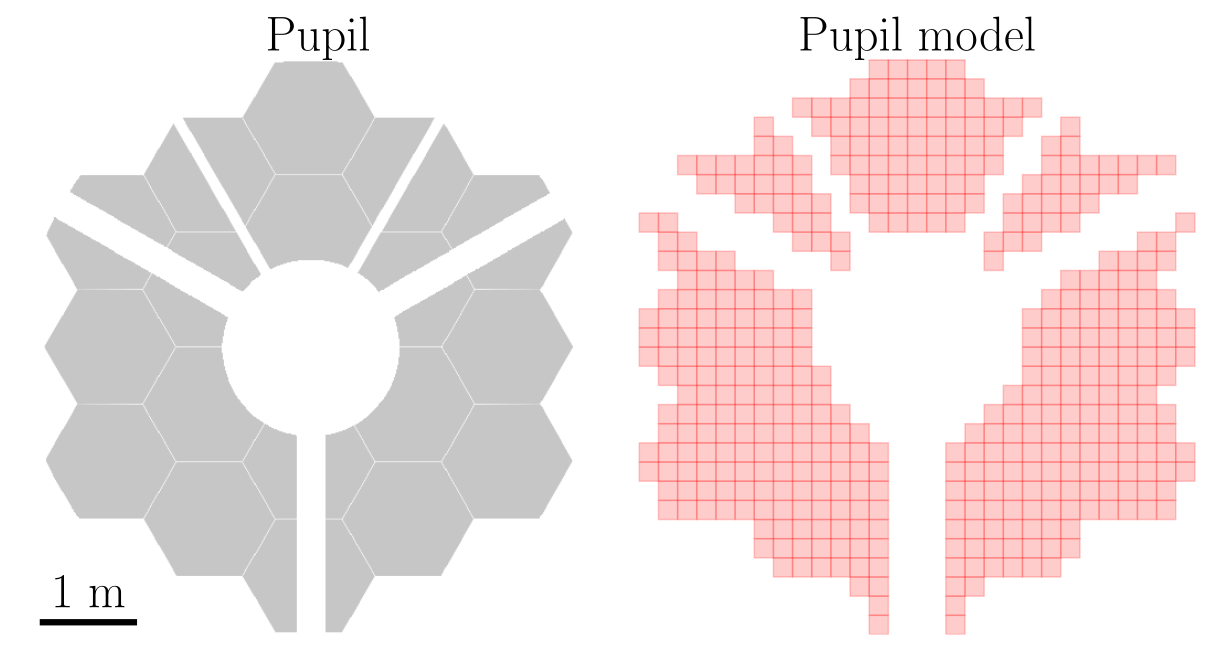
\includegraphics[width=0.9\linewidth]{figures/pupil_model.png}
%   \end{center}
% \end{frame}

% %% Instead of aperture mask, approximate pupil as many finite apertures
% \begin{frame}{Frequency coverage}
%
%   Analogous to the MTF we were computing earlier
%
%   \begin{center}
%     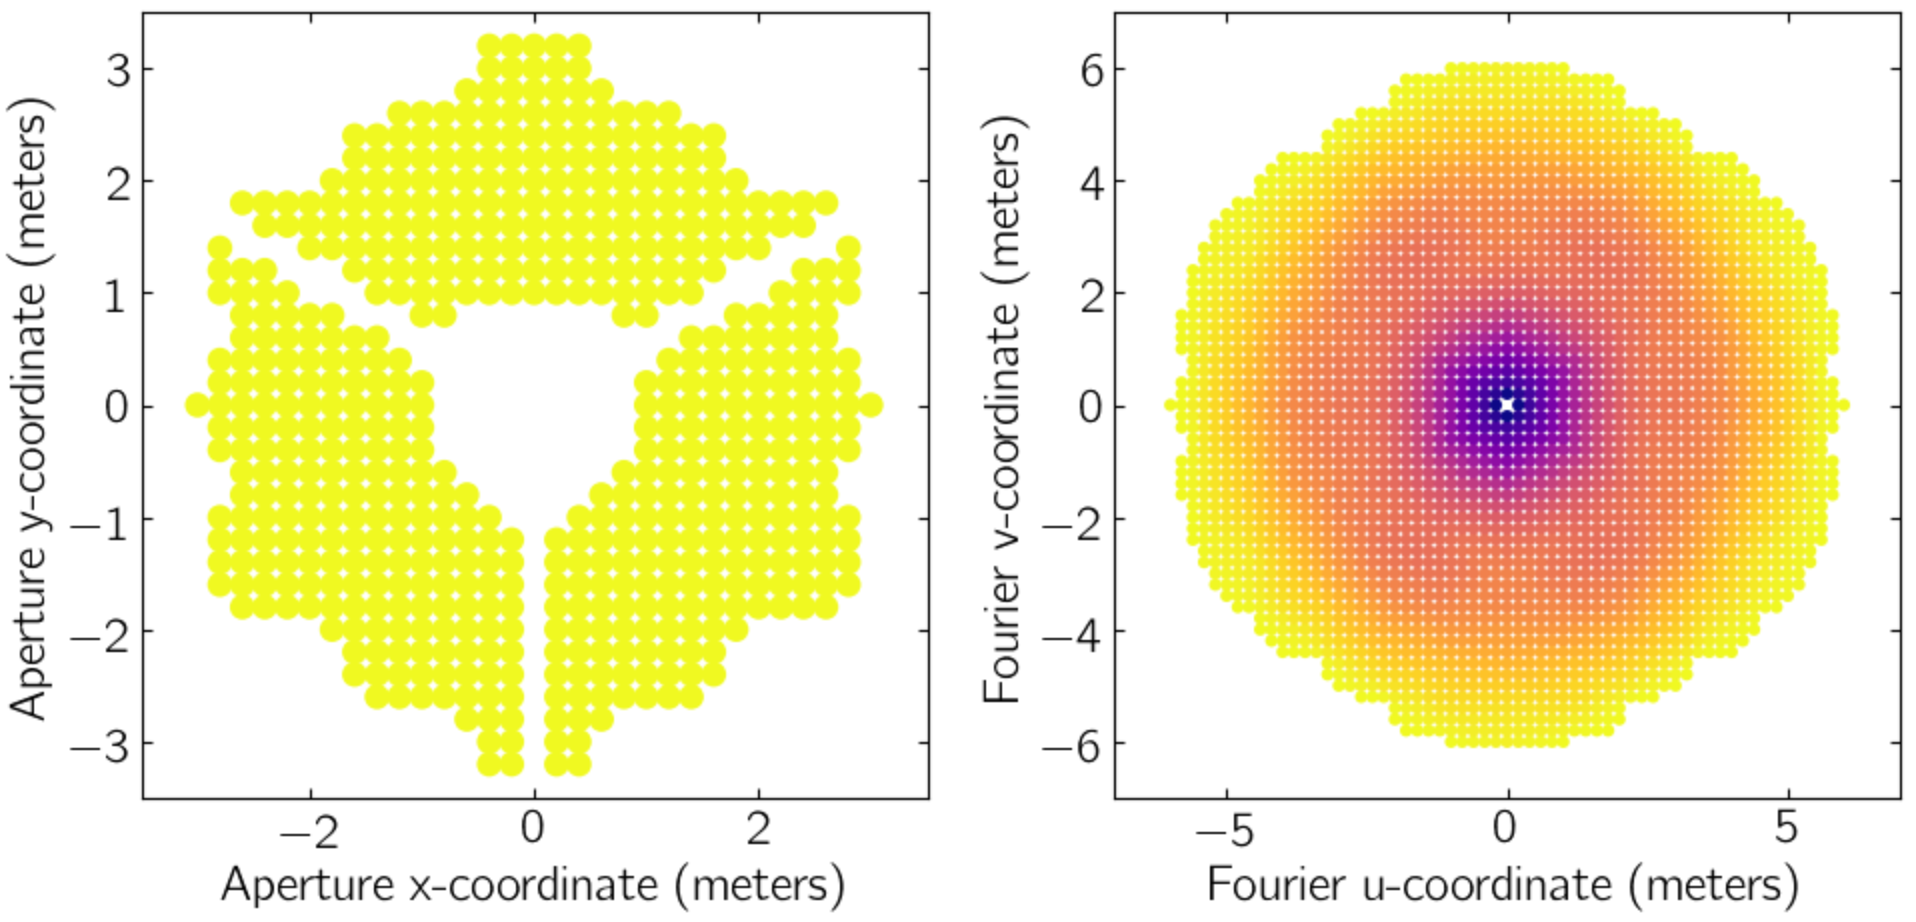
\includegraphics[width=0.9\linewidth]{figures/discrete_pupil_uv.png}
%   \end{center}
% \end{frame}
%
% \begin{frame}{Kernel phase analysis}
%   \begin{wideitemize}
%     \item<1-> Observe target
%     \item<2-> Calculate \vect{K} from pupil geometry
%     \item<3-> Extract kernel phases \vect{K} \boldsymbol{\Phi}
%     \item<4-> Generate model kernel phases \vect{K} \boldsymbol{\Phi}^O
%     \item<5-> Fit model KP to observed KP
%     \item<6-> Detect companion !
%   \end{wideitemize}
% \end{frame}

% \begin{frame}{Summary}
%   Both AMI and Kernel:
%   \begin{wideitemize}
%     \item<1-> Observables immune to phase errors
%     \item<2-> Enable direct detection at separations below $\lambda/D$
%   \end{wideitemize}
%   AMI:
%   \begin{wideitemize}
%     \item<3-> Non-redundant pupil mask
%     \item<4-> Throughput of $\sim$ 5-15 \%
%     \item<5-> Small number of observables (limited by number of apertures)
%   \end{wideitemize}
%   Kernel:
%   \begin{wideitemize}
%     \item<6-> Uses the full pupil
%     \item<7-> Requires high Strehl ratio (space or AO)
%   \end{wideitemize}
% \end{frame}

% TODO: Use clearp pupil here
% Go back to a full pupil image. This is image and info we would get
% Imagine have star near core
\begin{frame}{NIRISS AMI PSF and Spatial Frequencies}
  % First way to think about this: "high pass filter"
  \only<1>{
    \begin{center}
      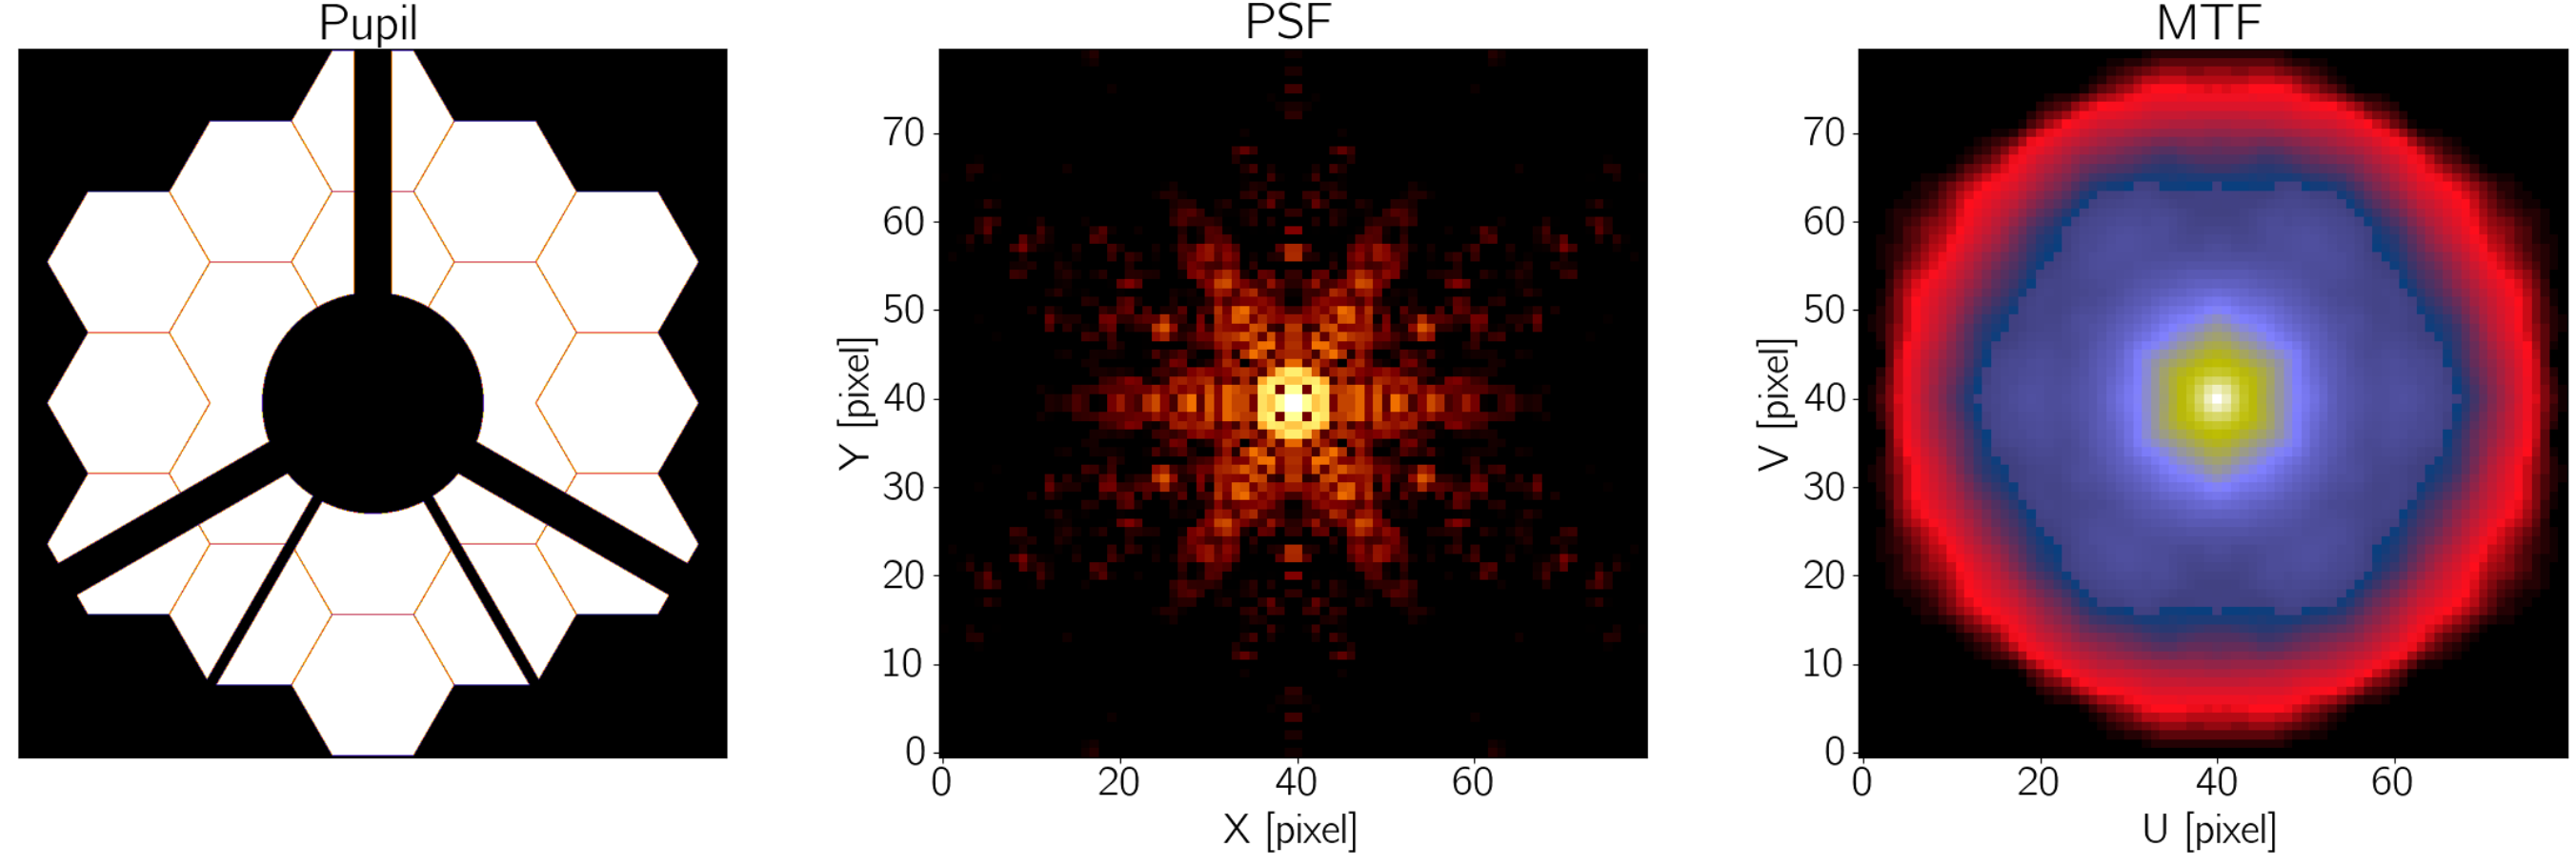
\includegraphics[width=\linewidth]{figures/analyse_niriss_clear.png}
    \end{center}
  }
  \only<2>{
    \begin{center}
      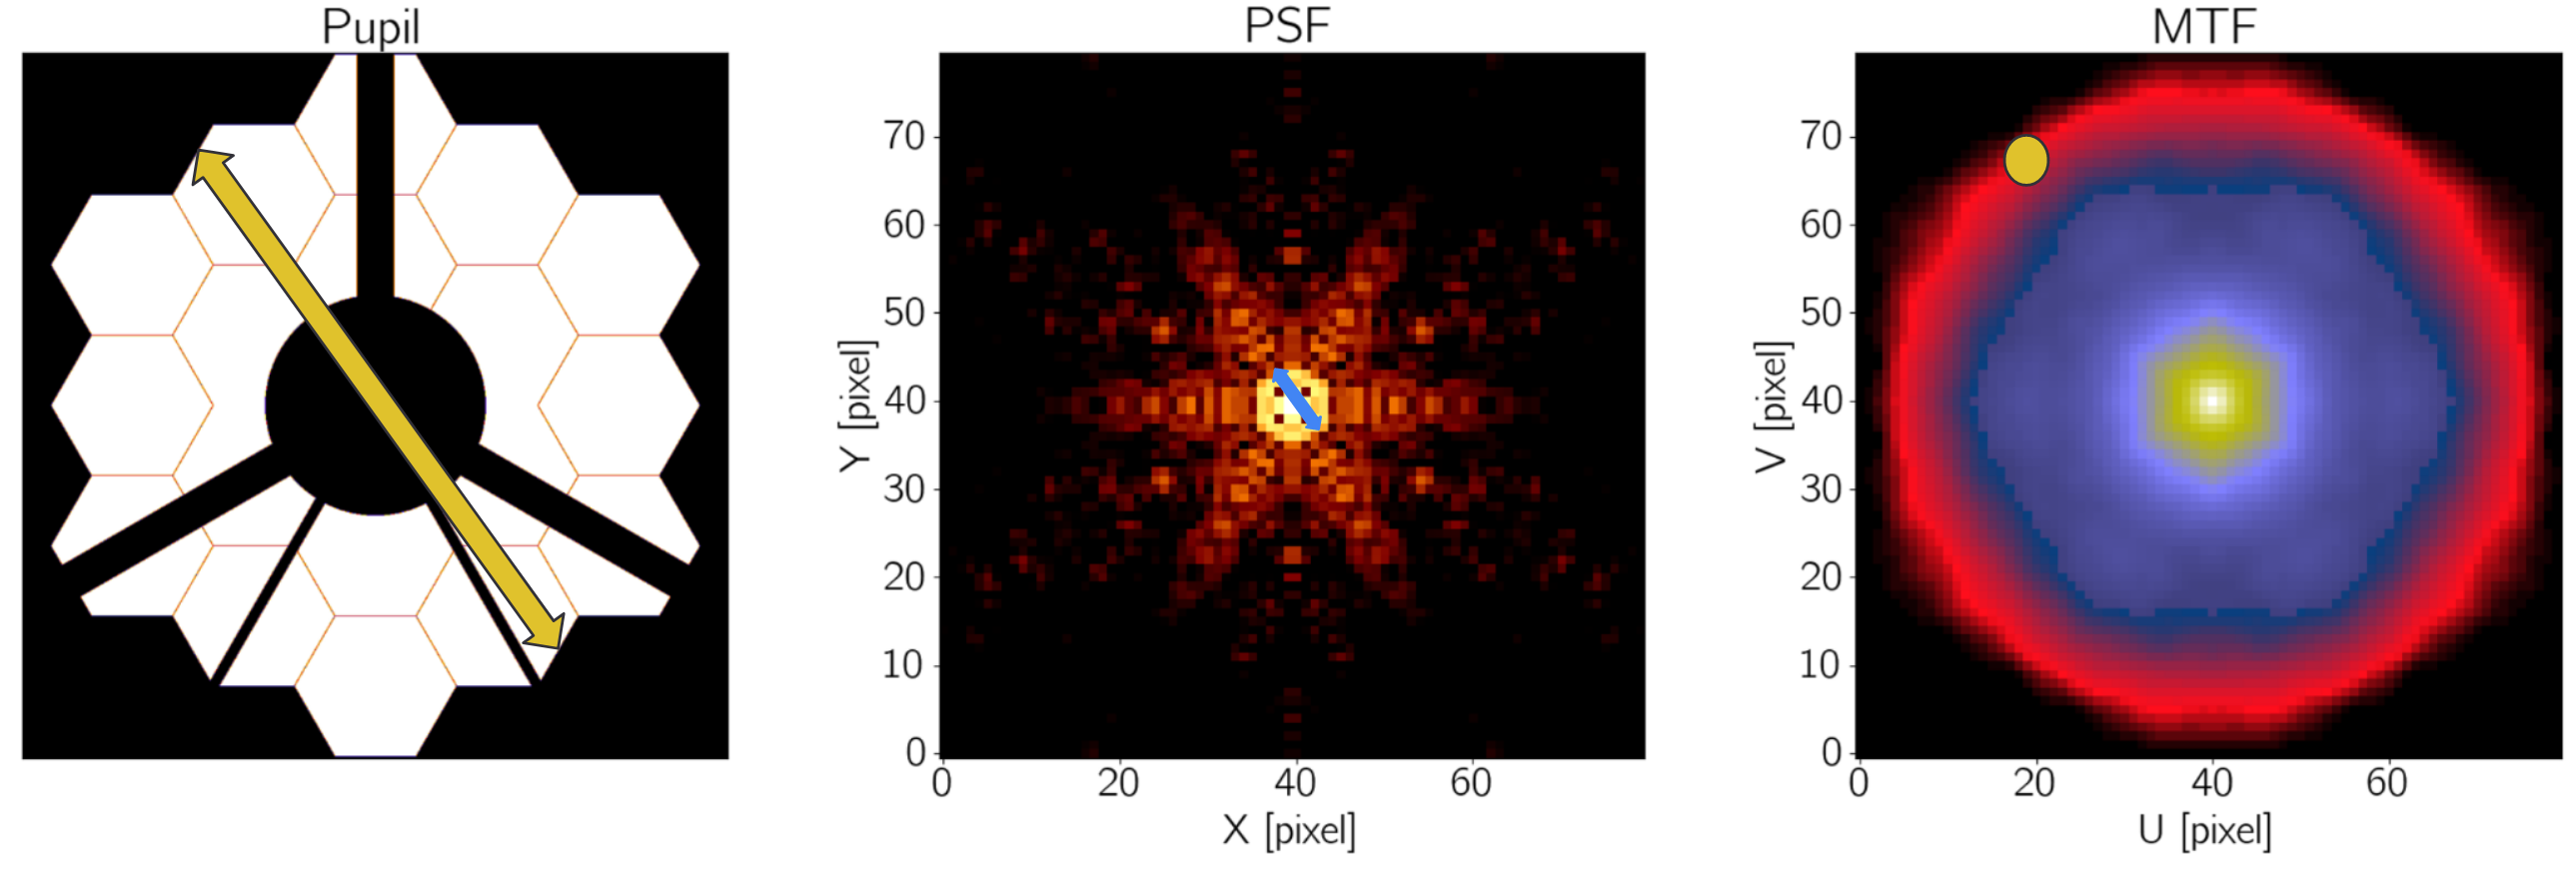
\includegraphics[width=\linewidth]{figures/clear_long_baseline.png}
    \end{center}
  }
  \only<3>{
    \begin{center}
      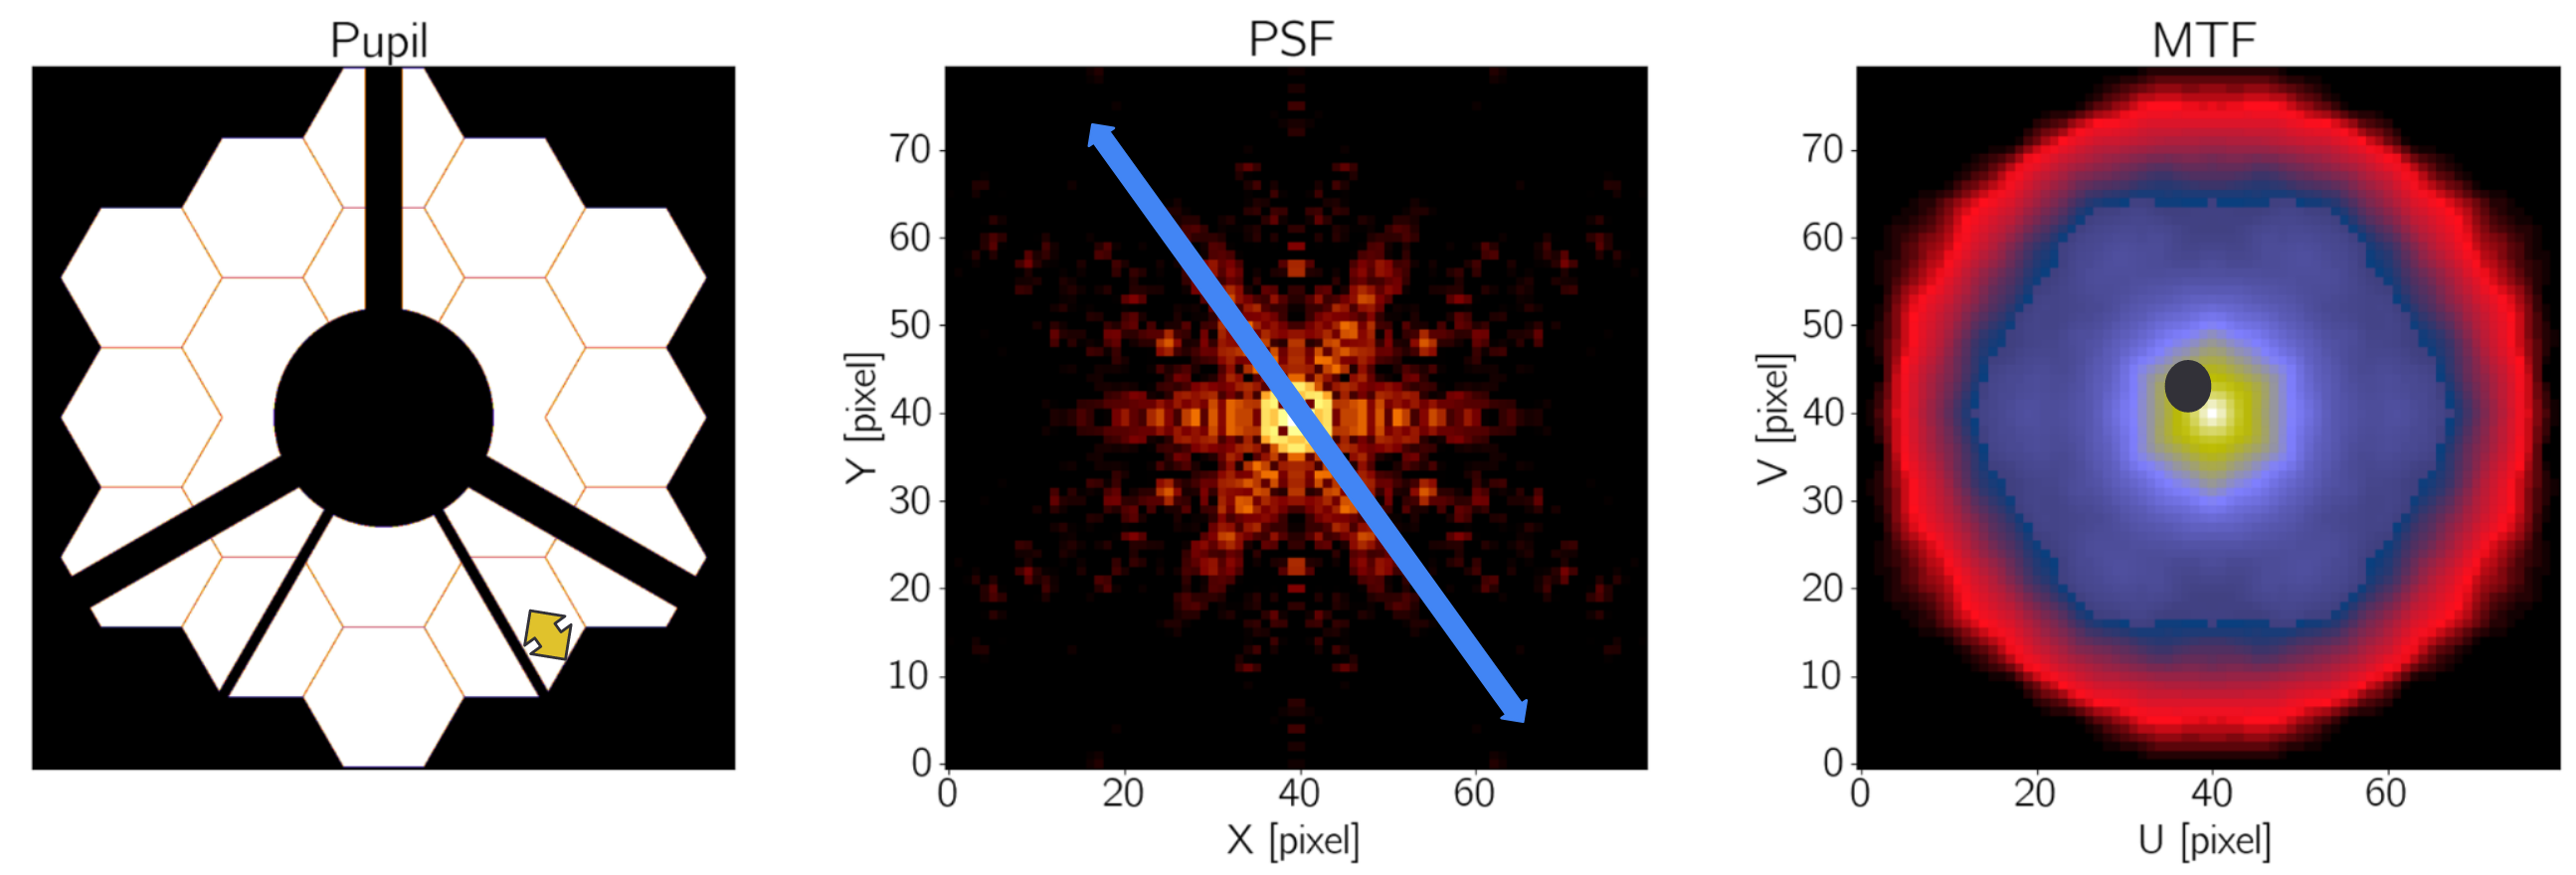
\includegraphics[width=\linewidth]{figures/clear_short_baseline.png}
    \end{center}
  }
\end{frame}

\begin{frame}{NIRISS AMI PSF and Spatial Frequencies}
  \only<1>{
    \begin{center}
      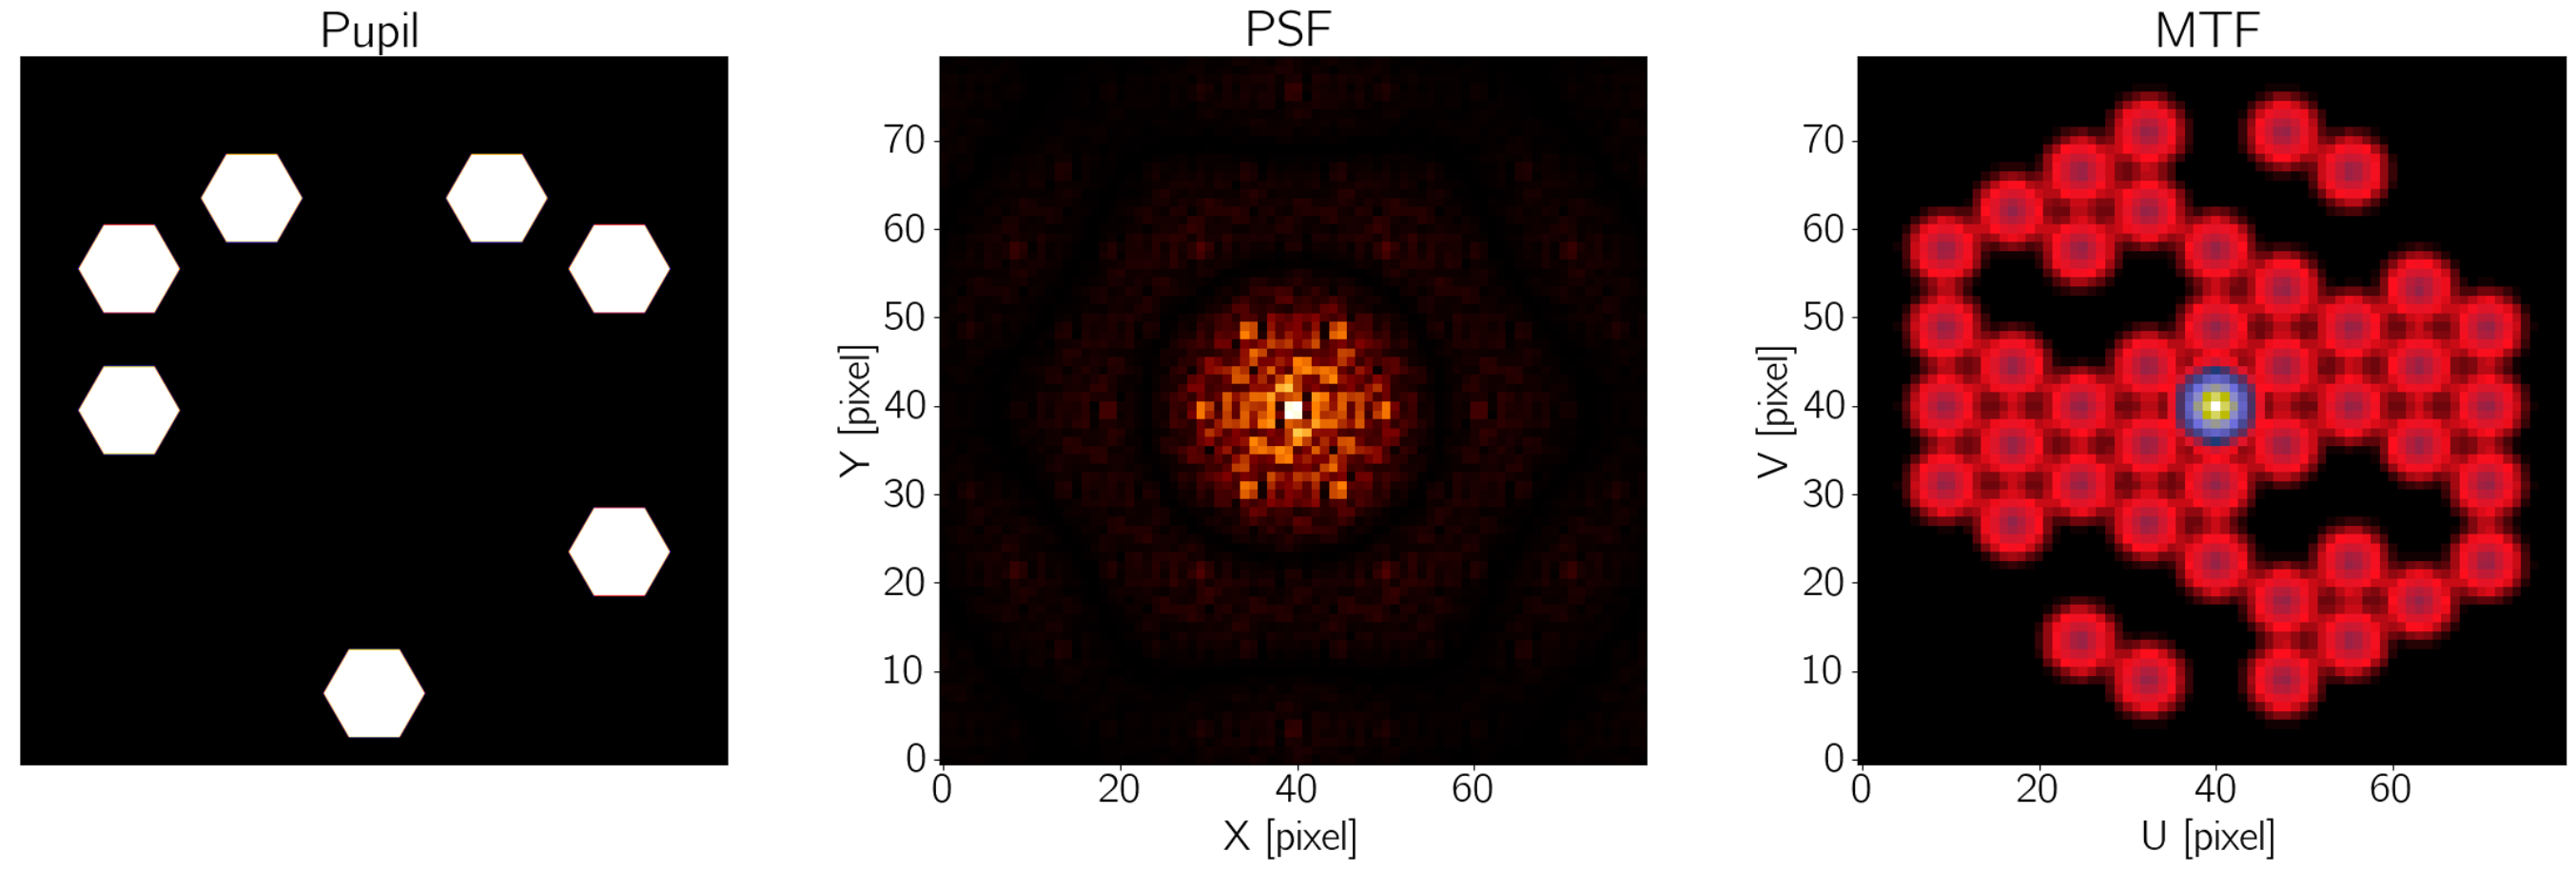
\includegraphics[width=\linewidth]{figures/analyse_niriss_ami.png}
    \end{center}
  }
  \only<2>{
    First way to think about this: "high pass filter"
    \begin{center}
      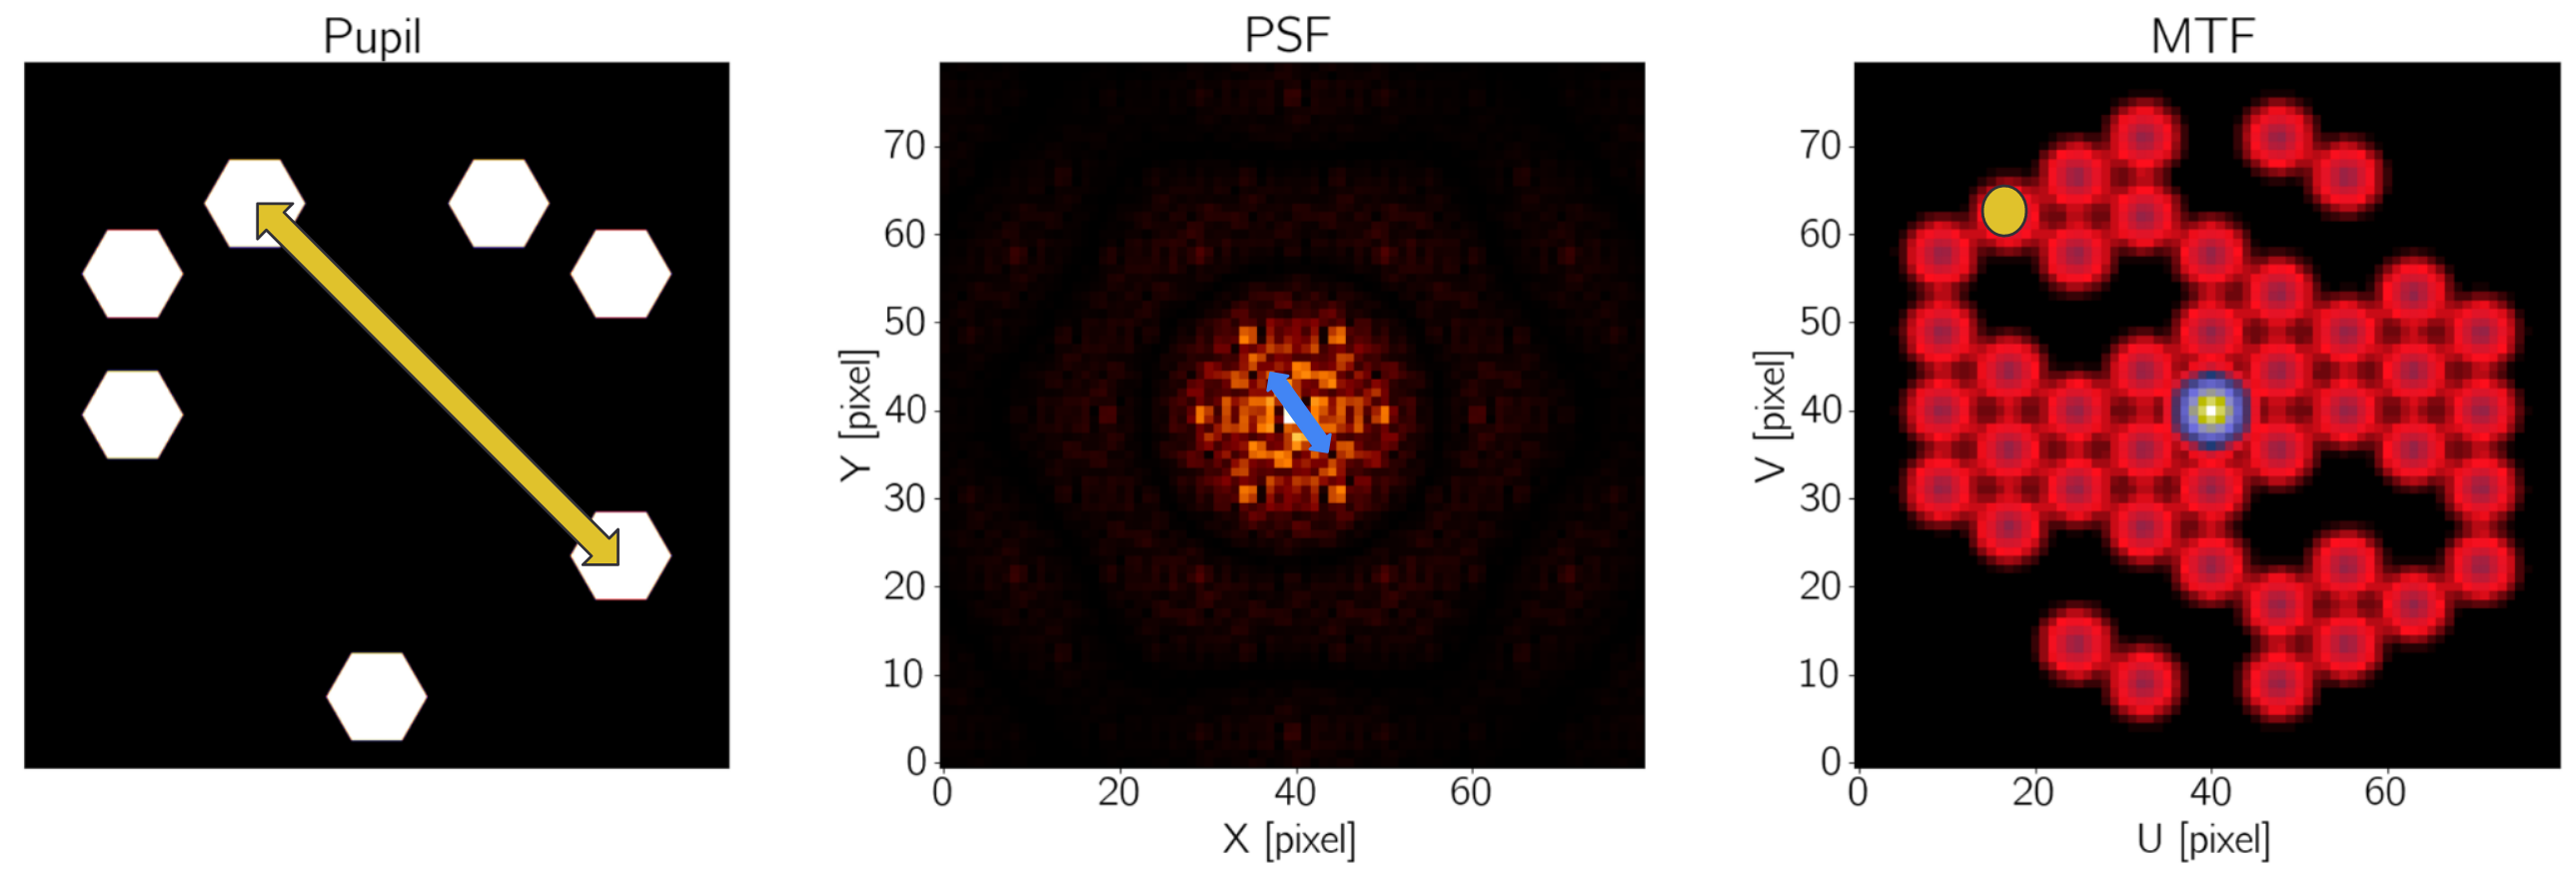
\includegraphics[width=\linewidth]{figures/ami_long_baseline.png}
    \end{center}
  }
  \only<3>{
    But most importantly: self-calibration
    \begin{center}
      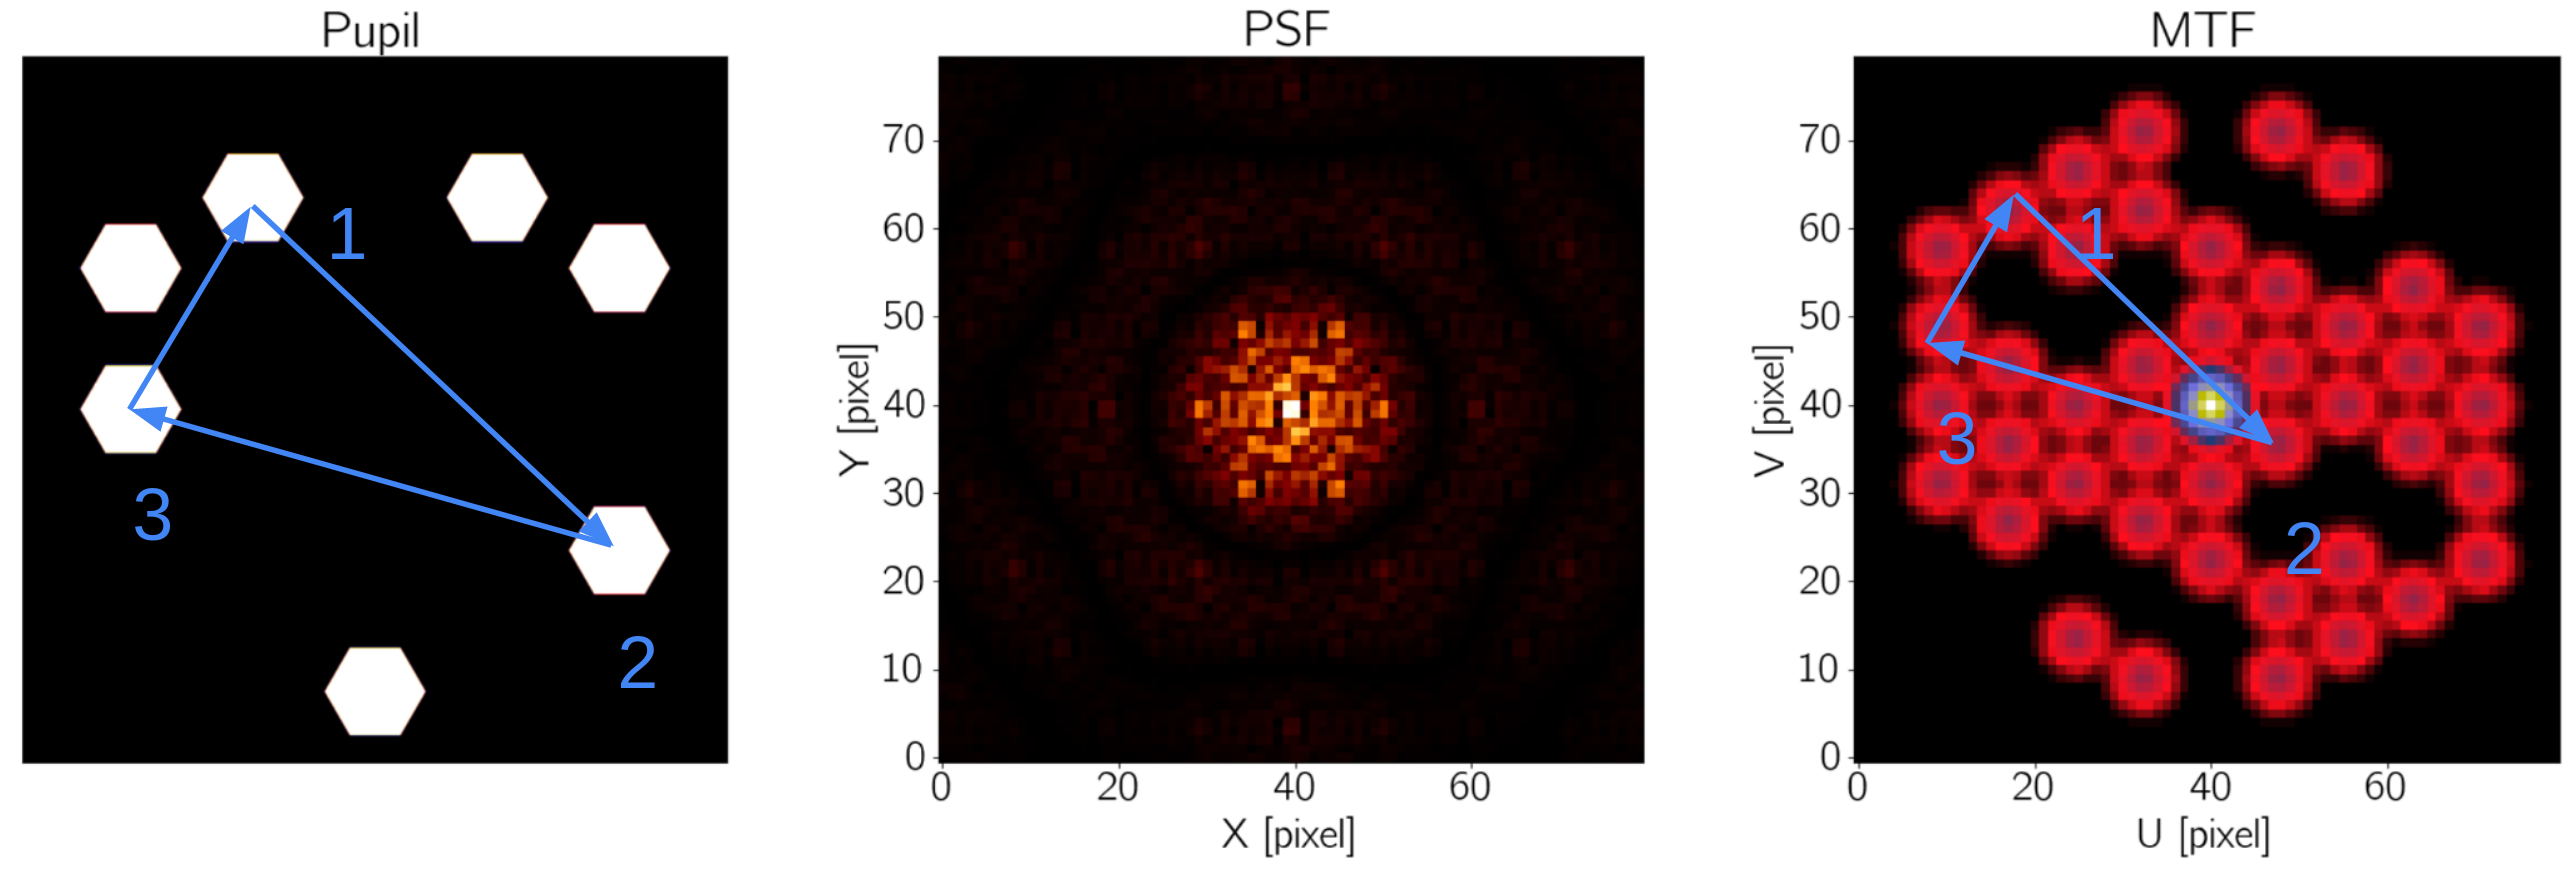
\includegraphics[width=\linewidth]{figures/ami_triagnle.png}
    \end{center}
  }
\end{frame}
%% Can also apply to NRM Mask
\begin{frame}{Closure phase}

\begin{columns}
\column{0.6\textwidth}

  \only<1>{
    \begin{align*}
      &\Phi_{1,2} = \Phi_{1,2}^O + \phi_2 \\
      &\Phi_{2,3} = \Phi_{2,3}^O + \phi_3 - \phi_2 \\
      &\Phi_{3,1} = \Phi_{3,1}^O - \phi_3
    \end{align*}
  }
  \only<2->{
    \begin{align*}
      &\Phi_{1,2} = \Phi_{1,2}^O + \cancel{\phi_2} \\
      &\Phi_{2,3} = \Phi_{2,3}^O + \cancel{\phi_3} - \cancel{\phi_2} \\
      &\Phi_{3,1} = \Phi_{3,1}^O - \cancel{\phi_3}
    \end{align*}
  }

  \begin{equation*}
    C_{123} = \Phi_{1,2} + \Phi_{2,3} + \Phi_{3,1} = \Phi_{1,2}^O + \Phi_{2,3}^O + \Phi_{3,1}^O
  \end{equation*}

\column{0.4\textwidth}
  \onslide<1->{
    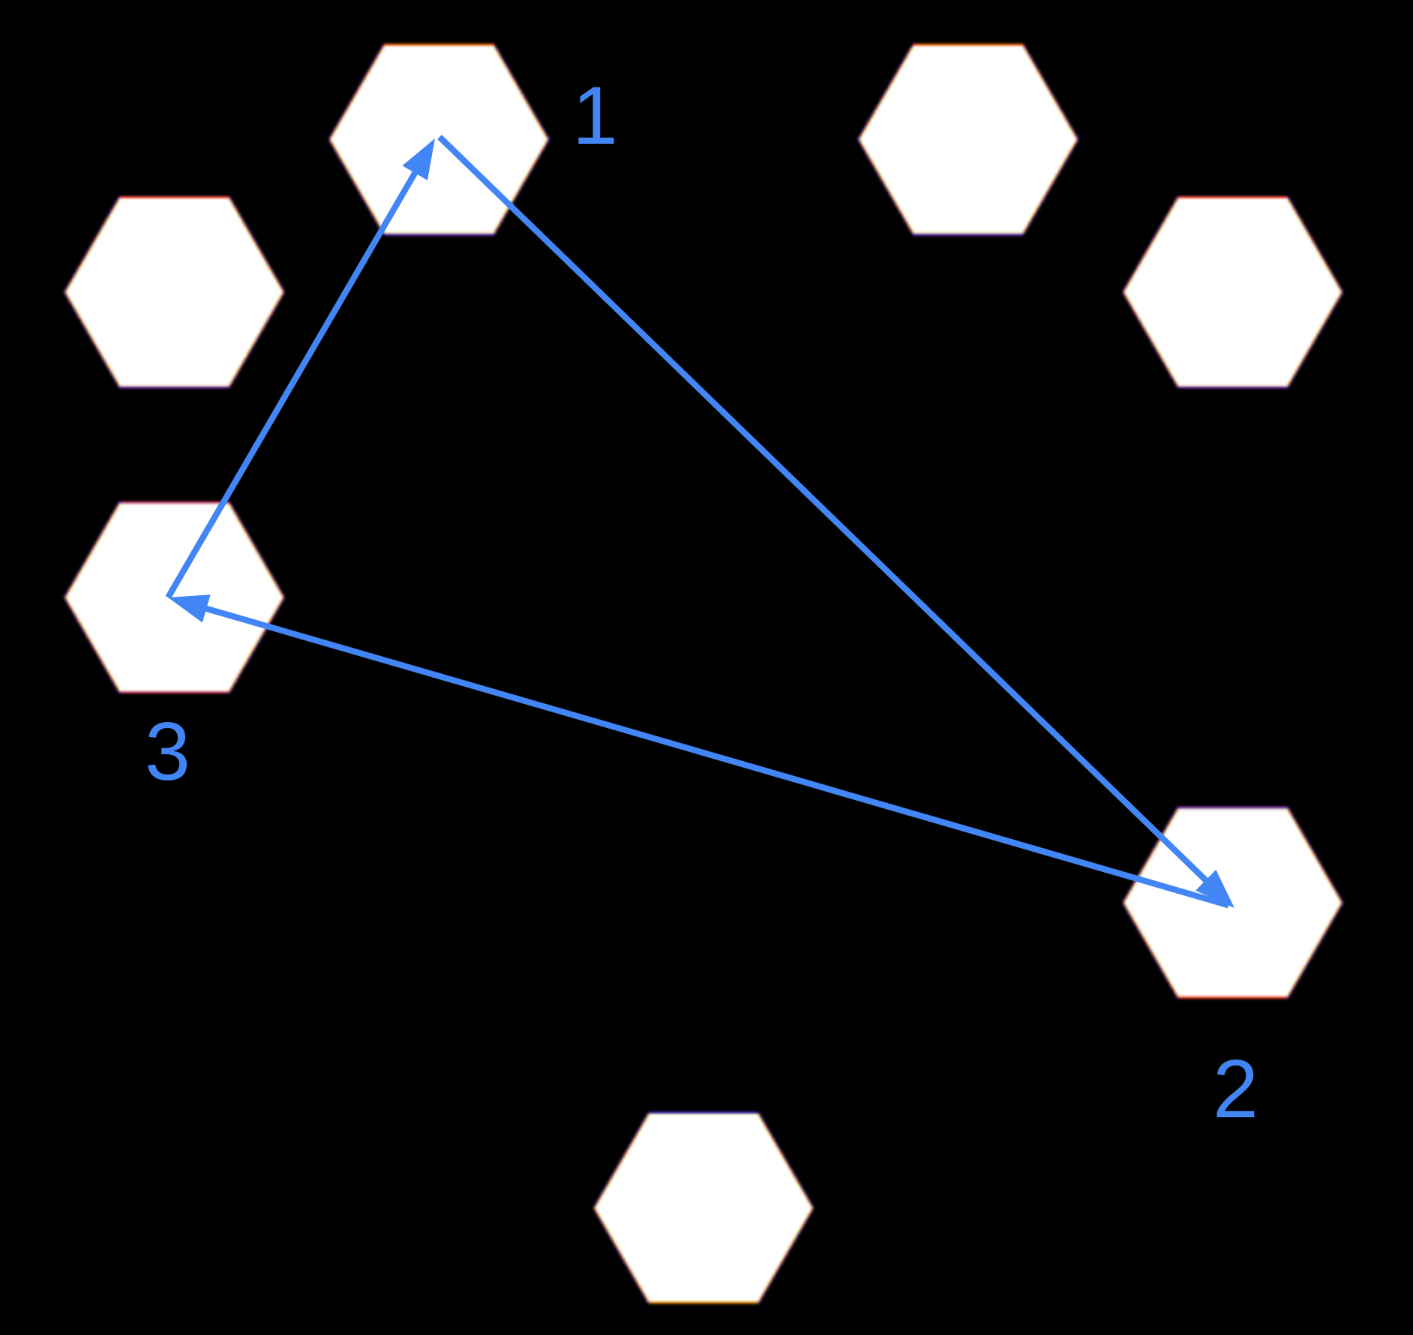
\includegraphics[width=\linewidth]{figures/nrm_pupil_triangle.png}
  }
\end{columns}

\end{frame}


pend{document}
